\pdfminorversion=4 % for acroread
%\documentclass[aspectratio=169,t,xcolor={usenames,dvipsnames}]{beamer}
\documentclass[aspectratio=169,t,handout,xcolor={usenames,dvipsnames}]{beamer}
\usepackage{../beamerstyle}
\usepackage{dsfont}
\usepackage{bm}
\usepackage[english]{babel}
\usepackage[utf8]{inputenc}
\usepackage{graphicx}
\usepackage{algorithm}
\usepackage[ruled,vlined,algo2e,linesnumbered]{algorithm2e}
%\usepackage[boxed,vlined]{algorithm2e}
\usepackage{hyperref}
\usepackage{booktabs}
\usepackage{mathtools}

\usepackage{amsmath,amssymb}
\usepackage{listings}
\lstset{frame=lines,framesep=3pt,numbers=left,numberblanklines=false,basicstyle=\ttfamily\small}

\usepackage{subfig}
\usepackage{multicol}
%\usepackage{appendixnumberbeamer}
%
\usepackage{tcolorbox}

\usepackage{pgfplots}
\usepackage{tikz}
\usetikzlibrary{trees} 
\usetikzlibrary{shapes.geometric}
\usetikzlibrary{positioning,shapes,shadows,arrows,calc,mindmap}
\usetikzlibrary{positioning,fadings,through}
\usetikzlibrary{decorations.pathreplacing}
\usetikzlibrary{intersections}
\usetikzlibrary{positioning,fit,calc,shadows,backgrounds}
\pgfdeclarelayer{background}
\pgfdeclarelayer{foreground}
\pgfsetlayers{background,main,foreground}
\tikzstyle{activity}=[rectangle, draw=black, rounded corners, text centered, text width=8em]
\tikzstyle{data}=[rectangle, draw=black, text centered, text width=8em]
\tikzstyle{myarrow}=[->, thick, draw=black]

% Define the layers to draw the diagram
\pgfdeclarelayer{background}
\pgfdeclarelayer{foreground}
\pgfsetlayers{background,main,foreground}

%\usepackage{listings}
%\lstset{numbers=left,
%  showstringspaces=false,
%  frame={tb},
%  captionpos=b,
%  lineskip=0pt,
%  basicstyle=\ttfamily,
%%  extendedchars=true,
%  stepnumber=1,
%  numberstyle=\small,
%  xleftmargin=1em,
%  breaklines
%}

 
\definecolor{blue}{RGB}{0, 74, 153}

\usetheme{Boadilla}
%\useinnertheme{rectangles}
\usecolortheme{whale}
\setbeamercolor{alerted text}{fg=blue}
\useoutertheme{infolines}
\setbeamertemplate{navigation symbols}{\vspace{-5pt}} % to lower the logo
\setbeamercolor{date in head/foot}{bg=white} % blue
\setbeamercolor{date in head/foot}{fg=white}
\setbeamercolor{author  in head/foot}{bg=white} %blue
\setbeamercolor{title in head/foot}{bg=white} % blue
\setbeamercolor{title}{fg=white, bg=blue}
\setbeamercolor{block title}{fg=white,bg=blue}
\setbeamercolor{block body}{bg=blue!10}
\setbeamercolor{frametitle}{fg=white, bg=blue}
\setbeamercovered{invisible}

\makeatletter
\setbeamertemplate{footline}
{
  \leavevmode%
  \hbox{%
  \begin{beamercolorbox}[wd=.333333\paperwidth,ht=2.25ex,dp=1ex,center]{author in head/foot}%
%    \usebeamerfont{author in head/foot}\insertshortauthor
  \end{beamercolorbox}%
  \begin{beamercolorbox}[wd=.333333\paperwidth,ht=2.25ex,dp=1ex,center]{title in head/foot}%
    \usebeamerfont{title in head/foot}\insertshorttitle
  \end{beamercolorbox}%
  \begin{beamercolorbox}[wd=.333333\paperwidth,ht=2.25ex,dp=1ex,right]{date in head/foot}%
    \usebeamerfont{date in head/foot}\insertshortdate{}\hspace*{2em}
%    \insertframenumber\hspace*{2ex} 
  \end{beamercolorbox}}%
  \vskip0pt%
}
\makeatother

%\pgfdeclareimage[height=1.2cm]{automl}{images/logos/automl.png}
%\pgfdeclareimage[height=1.2cm]{freiburg}{images/logos/freiburg}

%\logo{\pgfuseimage{freiburg}}

\renewcommand{\comment}[1]{
	\noindent
	%\vspace{0.25cm}
	{\color{red}{\textbf{TODO:} #1}}
	%\vspace{0.25cm}
}
\newcommand{\notefh}[1]{\textcolor{red}{\textbf{FH:} #1}}
\renewcommand{\comment}[1]{}
\newcommand{\hide}[1]{}
\newcommand{\cemph}[2]{\emph{\textcolor{#1}{#2}}}

\newcommand{\lit}[1]{{\footnotesize\color{black!60}[#1]}}

\newcommand{\litw}[1]{{\footnotesize\color{blue!20}[#1]}}


\newcommand{\myframe}[2]{\begin{frame}[c]{#1}#2\end{frame}}
\newcommand{\myframetop}[2]{\begin{frame}{#1}#2\end{frame}}
\newcommand{\myit}[1]{\begin{itemize}#1\end{itemize}}
\newcommand{\myblock}[2]{\begin{block}{#1}#2\end{block}}


\newcommand{\votepurple}[1]{\textcolor{Purple}{$\bigstar$}}
\newcommand{\voteyellow}[1]{\textcolor{Goldenrod}{$\bigstar$}}
\newcommand{\voteblue}[1]{\textcolor{RoyalBlue}{$\bigstar$}}
\newcommand{\votepink}[1]{\textcolor{Pink}{$\bigstar$}}

\newcommand{\diff}{\mathop{}\!\mathrm{d}}
\newcommand{\refstyle}[1]{{\small{\textcolor{gray}{#1}}}}
\newcommand{\hands}[0]{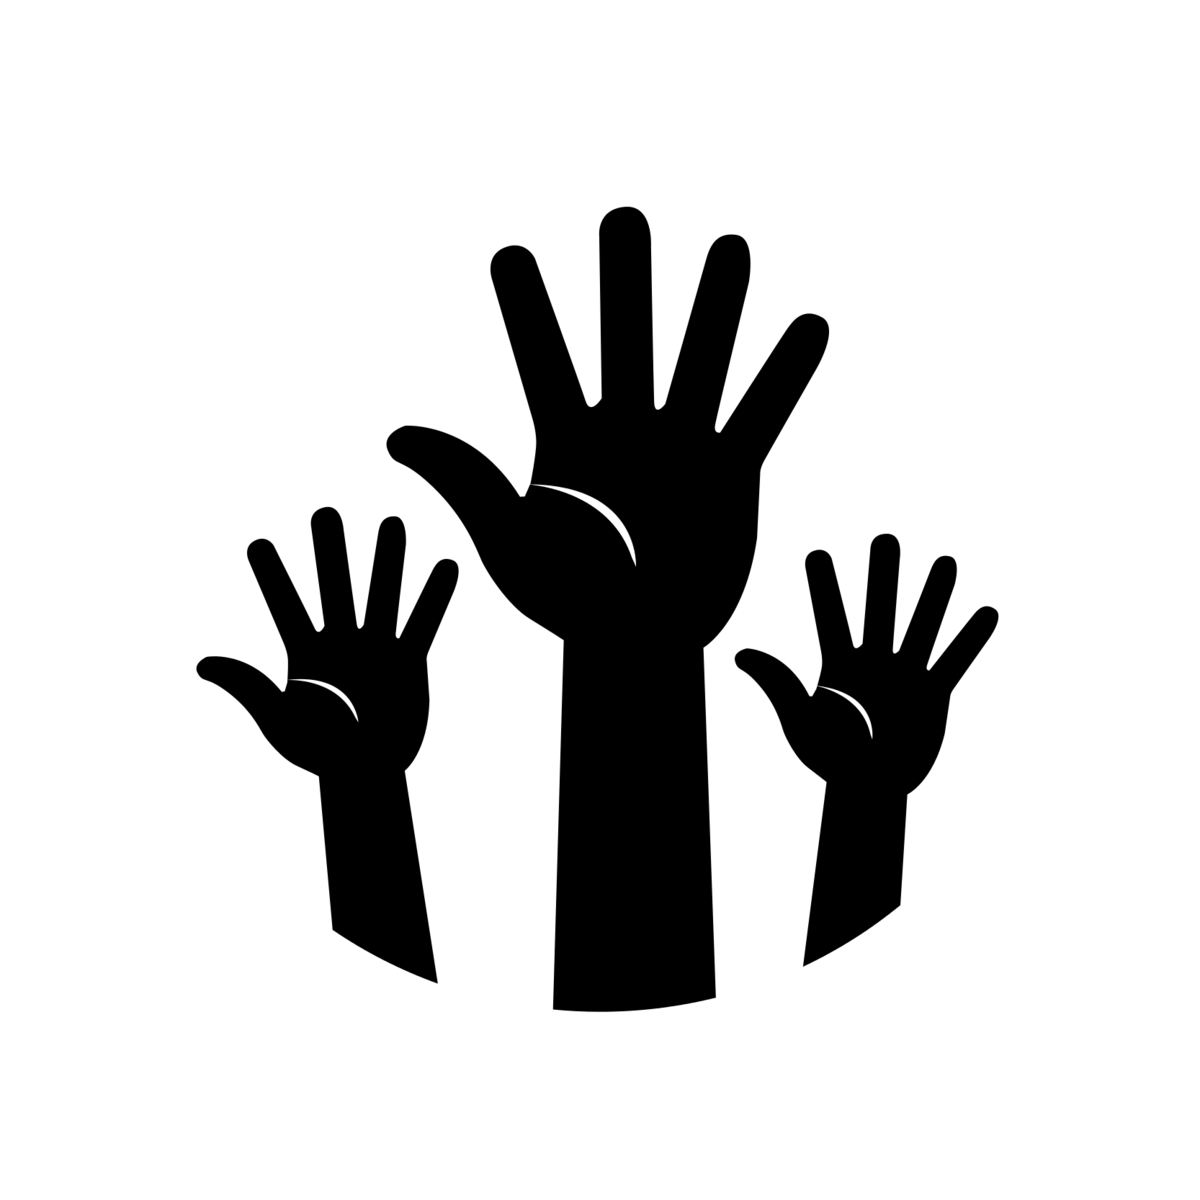
\includegraphics[height=1.5em]{images/hands}}
\newcommand{\transpose}[0]{{\textrm{\tiny{\sf{T}}}}}
\newcommand{\norm}{{\mathcal{N}}}
\newcommand{\cutoff}[0]{\kappa}
\newcommand{\instD}[0]{\dataset}
\newcommand{\insts}[0]{\mathcal{I}}
\newcommand{\inst}[0]{i}
\newcommand{\instI}[1]{i^{(#1)}}

% Iteration specific instance of variable/function/anything
% Introduced in the BO section, but moved up here to make it available within other macros
\newcommand{\iter}[2][\bocount]{{#2}^{(#1)}}

%--------HPO parameter macros-----------

% Parameter Configuration Space
\newcommand{\pcs}[0]{\pmb{\Lambda}}

% ???
\newcommand{\bx}[0]{\conf}

% Parameter Configuration
\newcommand{\conf}[0]{\pmb{\lambda}}

% Final Configuration
\newcommand{\finconf}[0]{\pmb{\hat{\lambda}}}

% Configuration corresponding to a given iteration -- better use \iter!
\newcommand{\confI}[1]{{\conf}^{(#1)}}

% Default Configuration
\newcommand{\defconf}[0]{{\conf}_{\text{def}}}

% Incumbent Configuration
\newcommand{\incumbent}[1][\bocount]{\iter[#1]{\finconf}}

% Optimal Configuration
\newcommand{\optconf}[0]{{\conf}^*}

% Configuration Space
\newcommand{\confs}[0]{\pcs}

%----------------------------------------

%\newcommand{\vlambda}[0]{\bm{\lambda}}
%\newcommand{\vLambda}[0]{\bm{\Lambda}}
\newcommand{\dataset}[0]{\mathcal{D}}
\newcommand{\datasets}[0]{\mathbf{D}}
\newcommand{\loss}[0]{L}
\newcommand{\risk}{\mathcal{R}}
\newcommand{\riske}{\mathcal{R}_{\text{emp}}}
\newcommand{\cost}[0]{c}
\newcommand{\costI}[1]{c^{(#1)}}

% Gaussian Process
\newcommand{\gp}{\mathcal{G}}
% Family of Objective Functions
\newcommand{\objF}{F}

%---------------BO Macros------------------

% BO loop counter
\newcommand{\bocount}{t}
% BO loop counter max, the counter runs from 1 to this value
\newcommand{\bobudget}{T}
% BO loop observation
\newcommand{\obs}[1][\conf]{\cost({#1})}
% BO loop observation space
\newcommand{\obsspace}{\mathcal{Y}}
% BO loop next observation
\newcommand{\bonextobs}{\obs[\iter{\conf}]}
% Acquisition Function, no args
\newcommand{\acq}{u}
% Standard Normal PDF
\newcommand{\pdf}{\phi}
% Standard Normal CDF
\newcommand{\cdf}{\Phi}
% Mean
\newcommand{\mean}{\mu}
% Standard Deviation
\newcommand{\stddev}{\sigma}
% Variance
\newcommand{\variance}{\sigma^2}
% Noise
\newcommand{\noise}{\nu}
% BO loop next selected sample
\newcommand{\bonextsample}{\confI{\bocount}}

% Single hyperparameter
\newcommand{\hyperparam}{\lambda}

% Single hyperparameter within a hyperparameter configuration
\newcommand{\hyperparami}[1][i]{{\hyperparam}_#1}

% Full definition of final configuration
\newcommand{\finconffull}{\incumbent[\bobudget]}

% Dataset
\newcommand{\datasetHPO}{{\dataset}_{HPO}}

% Dataset definition
\newcommand{\datasetHPOdef}{{\langle \bonextsample,\,\bonextobs \rangle}_{\bocount=1}^{\bobudget}}

% Double Display Fraction, forces large displays for everything in numerator and denominator
\newcommand\ddfrac[2]{\frac{\displaystyle #1}{\displaystyle #2}}

% Conditional Probability "Given That" Relation, source:https://tex.stackexchange.com/a/141685/205886
\newcommand\given[1][]{\:#1\vert\:}

% Expectation as a math operator
\DeclareMathOperator*{\E}{\mathbb{E}}

% Citation 
\newcommand{\source}[1]{
    \begin{flushright}
    	Source: \lit{#1}
    \end{flushright}
}
%-------------------------------------------

%Real numbers set
\newcommand{\realnum}{\mathbb{R}}
%Configuration space - do not use
%\newcommand{\configspace}{\Theta}
%Instances - do not use
%\newcommand{\instances}{\mathcal{I}}
%Expected value
\newcommand{\expectation}{\mathbb{E}}
%Kernel
\newcommand{\kernel}{\kappa}
%Constraint function
\newcommand{\constraintf}{c}
%Normal distribution
\newcommand{\normaldist}{\mathcal{N}}

% \renewcommand{\vec}[1]{\mathbf{#1}}
\newcommand{\hist}[0]{\dataset_{\text{Hist}}}
\newcommand{\param}[0]{p}
\newcommand{\algo}[0]{\mathcal{A}}
\newcommand{\algos}[0]{\mathbf{A}}
%\newcommand{\nn}[0]{N}
\newcommand{\feats}[0]{\mathcal{X}_{\text{meta}}}
\newcommand{\feat}[0]{\x_{\text{meta}}}
%\newcommand{\cluster}[0]{\vec{h}}
%\newcommand{\clusters}[0]{\vec{H}}
\newcommand{\perf}[0]{\mathbb{R}}
%\newcommand{\surro}[0]{\mathcal{S}}
\newcommand{\surro}[0]{\hat{\cost}}
\newcommand{\func}[0]{f}
\newcommand{\epm}[0]{\surro}
\newcommand{\portfolio}[0]{\mathbf{P}}
\newcommand{\schedule}[0]{\mathcal{S}}

% Machine Learning
\newcommand{\mdata}[0]{\dataset_{\text{meta}}}
\newcommand{\datasettrain}[0]{\dataset_{\text{train}}}
\newcommand{\datasetval}[0]{\dataset_{\text{val}}}
\newcommand{\datasettest}[0]{\dataset_{\text{test}}}
\newcommand{\x}[0]{\mathbf{x}}
\newcommand{\y}[0]{y}
\newcommand{\xI}[1]{\mathbf{x}^{(#1)}}
\newcommand{\yI}[1]{y^{(#1)}}
\newcommand{\fx}{f(\mathbf{x})}  % f(x), continuous prediction function
\newcommand{\Hspace}{\mathcal{H}} % hypothesis space where f is from
\newcommand{\fh}{\hat{f}}       % f hat, estimated prediction function

% Deep Learning
\newcommand{\weights}[0]{\theta}
\newcommand{\metaweights}[0]{\phi}


% reinforcement learning
\newcommand{\policies}[0]{\mathbf{\Pi}}
\newcommand{\policy}[0]{\pi}
\newcommand{\actionRL}[0]{a}
\newcommand{\stateRL}[0]{s}
\newcommand{\statesRL}[0]{\mathcal{S}}
\newcommand{\rewardRL}[0]{r}
\newcommand{\rewardfuncRL}[0]{\mathcal{R}}

\RestyleAlgo{algoruled}
\DontPrintSemicolon
\LinesNumbered
\SetAlgoVlined
\SetFuncSty{textsc}

\SetKwInOut{Input}{Input}
\SetKwInOut{Output}{Output}
\SetKw{Return}{return}

%\newcommand{\changed}[1]{{\color{red}#1}}

%\newcommand{\citeN}[1]{\citeauthor{#1}~(\citeyear{#1})}

\renewcommand{\vec}[1]{\mathbf{#1}}
\DeclareMathOperator*{\argmin}{arg\,min}
\DeclareMathOperator*{\argmax}{arg\,max}

%\newcommand{\aqme}{\textit{AQME}}
%\newcommand{\aslib}{\textit{ASlib}}
%\newcommand{\llama}{\textit{LLAMA}}
%\newcommand{\satzilla}{\textit{SATzilla}}
%\newcommand{\satzillaY}[1]{\textit{SATzilla'{#1}}}
%\newcommand{\snnap}{\textit{SNNAP}}
%\newcommand{\claspfolioTwo}{\textit{claspfolio~2}}
%\newcommand{\flexfolio}{\textit{FlexFolio}}
%\newcommand{\claspfolioOne}{\textit{claspfolio~1}}
%\newcommand{\isac}{\textit{ISAC}}
%\newcommand{\eisac}{\textit{EISAC}}
%\newcommand{\sss}{\textit{3S}}
%\newcommand{\sunny}{\textit{Sunny}}
%\newcommand{\ssspar}{\textit{3Spar}}
%\newcommand{\cshc}{\textit{CSHC}}
%\newcommand{\cshcpar}{\textit{CSHCpar}}
%\newcommand{\measp}{\textit{ME-ASP}}
%\newcommand{\aspeed}{\textit{aspeed}}
%\newcommand{\autofolio}{\textit{AutoFolio}}
%\newcommand{\cedalion}{\textit{Cedalion}}
\newcommand{\fanova}{\textit{fANOVA}}
\newcommand{\sbs}{\textit{SB}}
\newcommand{\oracle}{\textit{VBS}}

% like approaches
\newcommand{\claspfoliolike}[1]{\texttt{claspfolio-#1-like}}
\newcommand{\satzillalike}[1]{\texttt{SATzilla'#1-like}}
\newcommand{\isaclike}{\texttt{ISAC-like}}
\newcommand{\ssslike}{\texttt{3S-like}}
\newcommand{\measplike}{\texttt{ME-ASP-like}}

\newcommand{\irace}{\textit{I/F-race}}
\newcommand{\gga}{\textit{GGA}}
\newcommand{\smac}{\textit{SMAC}}
\newcommand{\paramils}{\textit{ParamILS}}
\newcommand{\spearmint}{\textit{Spearmint}}
\newcommand{\tpe}{\textit{TPE}}


\usepackage{pifont}
\newcommand{\itarrow}{\mbox{\Pisymbol{pzd}{229}}}
\newcommand{\ithook}{\mbox{\Pisymbol{pzd}{52}}}
\newcommand{\itcross}{\mbox{\Pisymbol{pzd}{56}}}
\newcommand{\ithand}{\mbox{\raisebox{-1pt}{\Pisymbol{pzd}{43}}}}

%\DeclareMathOperator*{\argmax}{arg\,max}

\newcommand{\ie}{{\it{}i.e.\/}}
\newcommand{\eg}{{\it{}e.g.\/}}
\newcommand{\cf}{{\it{}cf.\/}}
\newcommand{\wrt}{\mbox{w.r.t.}}
\newcommand{\vs}{{\it{}vs\/}}
\newcommand{\vsp}{{\it{}vs\/}}
\newcommand{\etc}{{\copyedit{etc.}}}
\newcommand{\etal}{{\it{}et al.\/}}

\newcommand{\pscProc}{{\bf procedure}}
\newcommand{\pscBegin}{{\bf begin}}
\newcommand{\pscEnd}{{\bf end}}
\newcommand{\pscEndIf}{{\bf endif}}
\newcommand{\pscFor}{{\bf for}}
\newcommand{\pscEach}{{\bf each}}
\newcommand{\pscThen}{{\bf then}}
\newcommand{\pscElse}{{\bf else}}
\newcommand{\pscWhile}{{\bf while}}
\newcommand{\pscIf}{{\bf if}}
\newcommand{\pscRepeat}{{\bf repeat}}
\newcommand{\pscUntil}{{\bf until}}
\newcommand{\pscWithProb}{{\bf with probability}}
\newcommand{\pscOtherwise}{{\bf otherwise}}
\newcommand{\pscDo}{{\bf do}}
\newcommand{\pscTo}{{\bf to}}
\newcommand{\pscOr}{{\bf or}}
\newcommand{\pscAnd}{{\bf and}}
\newcommand{\pscNot}{{\bf not}}
\newcommand{\pscFalse}{{\bf false}}
\newcommand{\pscEachElOf}{{\bf each element of}}
\newcommand{\pscReturn}{{\bf return}}

%\newcommand{\param}[1]{{\sl{}#1}}
\newcommand{\var}[1]{{\it{}#1}}
\newcommand{\cond}[1]{{\sf{}#1}}
%\newcommand{\state}[1]{{\sf{}#1}}
%\newcommand{\func}[1]{{\sl{}#1}}
\newcommand{\set}[1]{{\Bbb #1}}
%\newcommand{\inst}[1]{{\tt{}#1}}
\newcommand{\myurl}[1]{{\small\sf #1}}

\newcommand{\Nats}{{\Bbb N}}
\newcommand{\Reals}{{\Bbb R}}
\newcommand{\extset}[2]{\{#1 \; | \; #2\}}

\newcommand{\vbar}{$\,\;|$\hspace*{-1em}\raisebox{-0.3mm}{$\,\;\;|$}}
\newcommand{\vendbar}{\raisebox{+0.4mm}{$\,\;|$}}
\newcommand{\vend}{$\,\:\lfloor$}


\newcommand{\goleft}[2][.7]{\parbox[t]{#1\linewidth}{\strut\raggedright #2\strut}}
\newcommand{\rightimage}[2][.3]{\mbox{}\hfill\raisebox{1em-\height}[0pt][0pt]{\includegraphics[width=#1\linewidth]{#2}}\vspace*{-\baselineskip}}






\title{AutoML: Bayesian Optimization for HPO}
\subtitle{Computationally Cheap Acquisition Functions}
\author[Marius Lindauer]{Bernd Bischl \and \underline{Frank Hutter} \and Lars Kotthoff\newline \and Marius Lindauer \and Joaquin Vanschoren}
\institute{}
\date{}

\begin{document}
\maketitle

%----------------------------------------------------------------------
\begin{frame}[c]{Acquisition Functions: the Basics}
\begin{itemize}
    \item Given the surrogate model $\iter{\surro}$ at the $\bocount$-th iteration of BO, the \\
    \alert{acquisition function $\acq(\cdot)$ judges the utility (or usefulness) of evaluating $f$ at $\iter{\conf}\in \pcs$ next}
    \pause
    \bigskip
    \item The acquisition function needs to \alert{trade off exploration and exploitation}
    \begin{itemize}
        \item E.g., just picking the $\conf$ with lowest predicted mean would be too greedy
        \item We also need to take into account the uncertainty of the surrogate model $\iter{\surro}$ to explore
    \end{itemize}
\end{itemize}

\end{frame}
%-----------------------------------------------------------------------
\begin{frame}[c]{Probability of Improvement (PI): Concept}

  {
    %\framesubtitle{Probability of Improvement - Concept}
    % \begin{figure}
      \centering
      \begin{tikzpicture}
        \node<+> (img1) {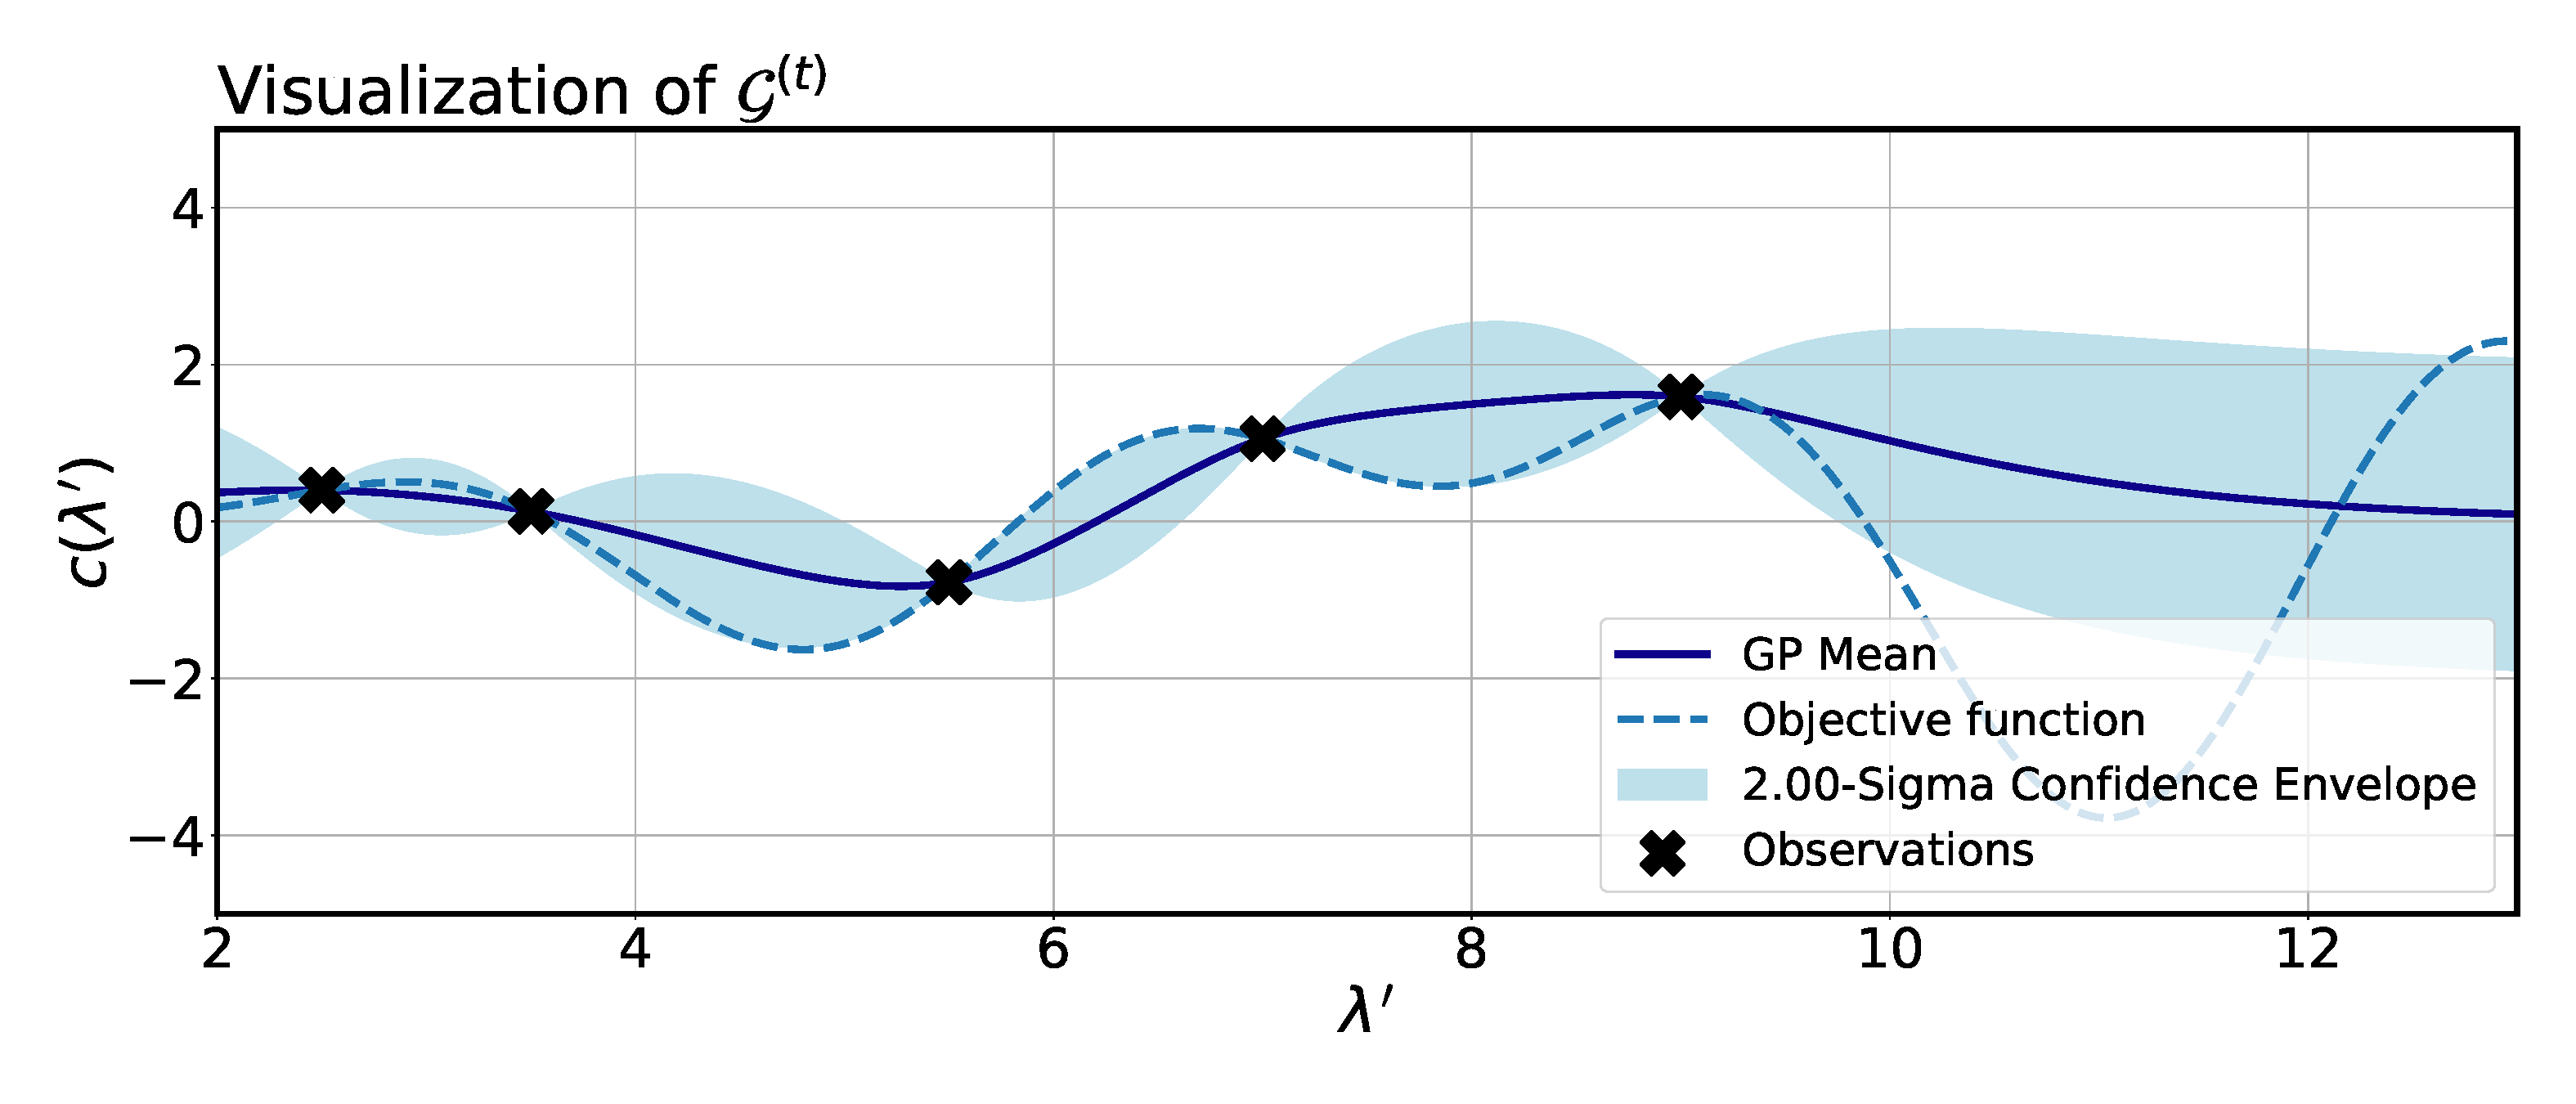
\includegraphics[width=\linewidth, height=0.7\textheight, keepaspectratio=true]{images/acq_func_images/pi/pi_1.pdf}};
        \node<.> [below=0.01\belowcaptionskip of img1, align=center]{Given the surrogate fit at iteration $\bocount$};
    
        \node<+> (img2) {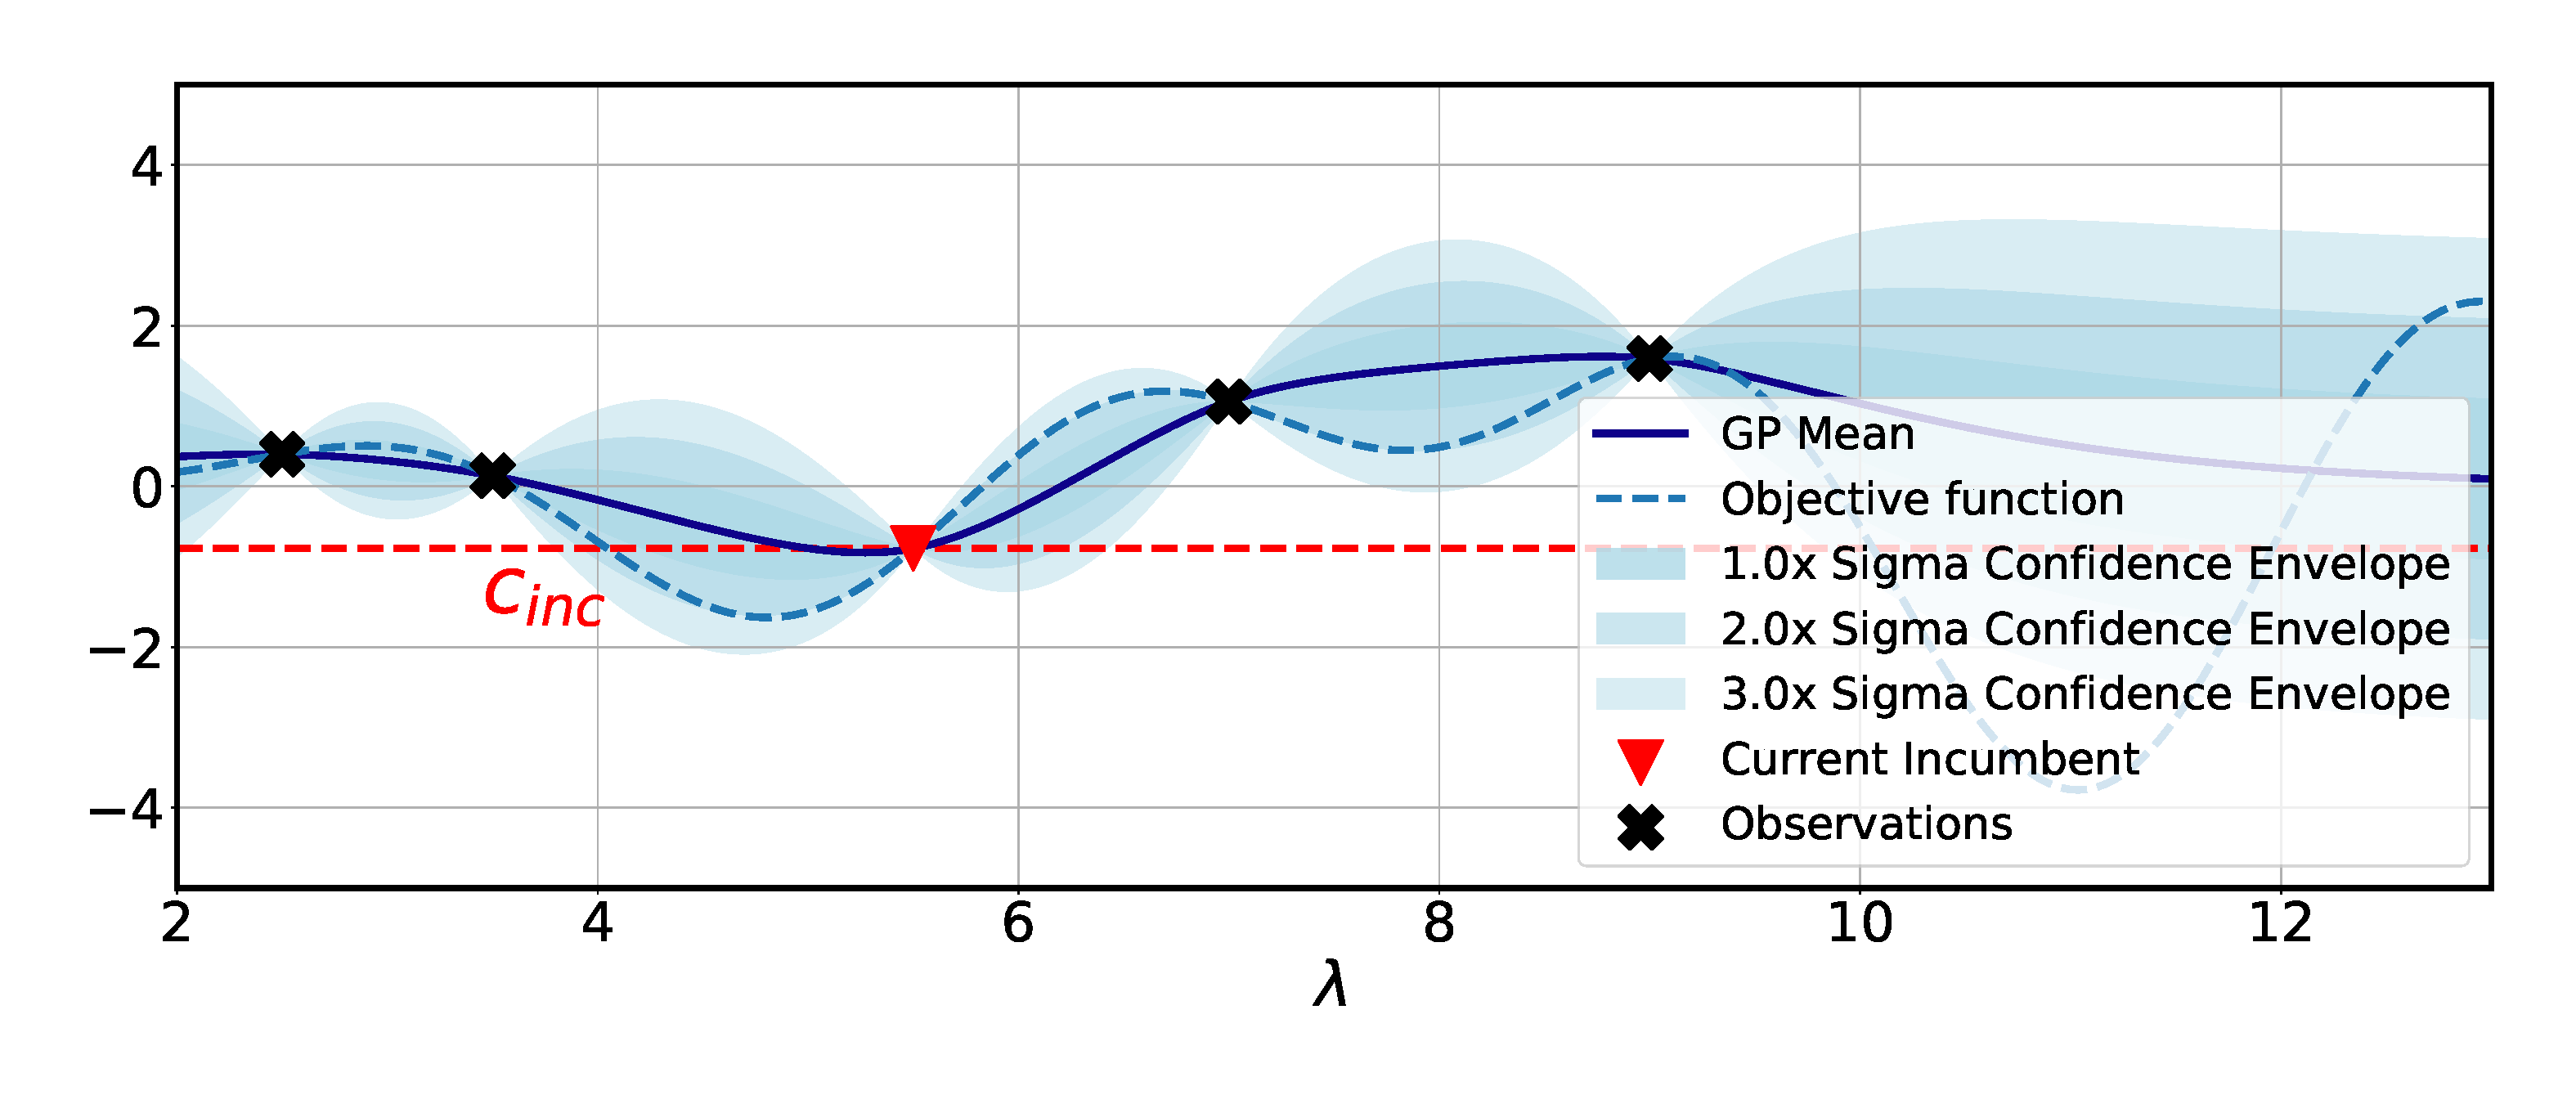
\includegraphics[width=\linewidth, height=0.7\textheight, keepaspectratio=true]{images/acq_func_images/pi/pi_2.pdf}};
        \node<.> [below=0.01\belowcaptionskip of img2, align=center]{Current incumbent $\hat{\conf}$ and its observed cost $\cost_{inc}$};
    
    
        \node<+> (img3) {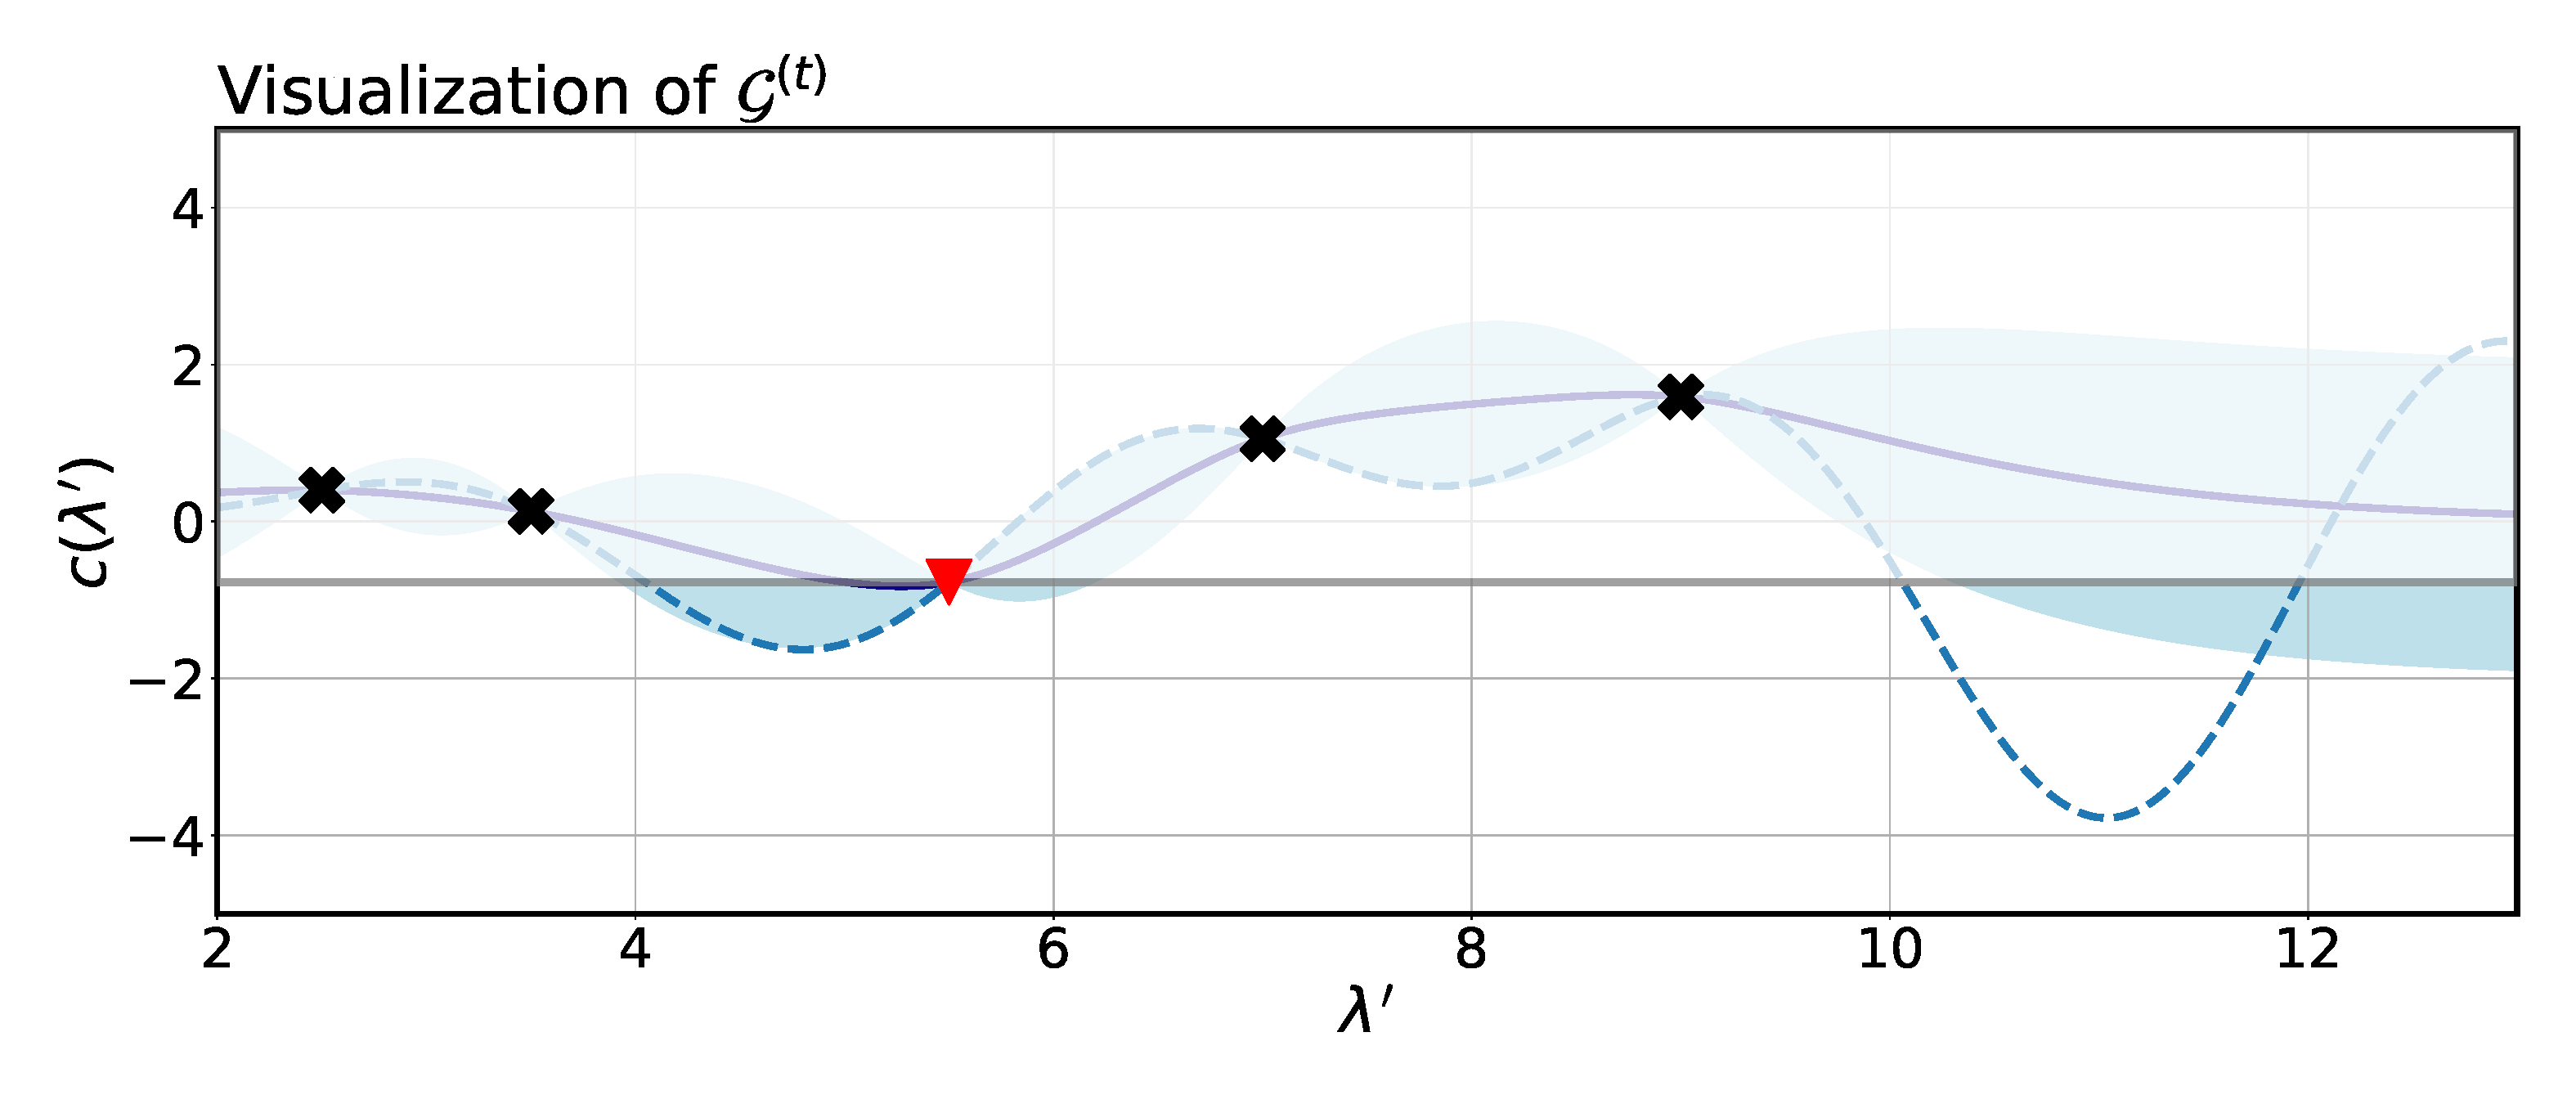
\includegraphics[width=\linewidth, height=0.7\textheight, keepaspectratio=true]{images/acq_func_images/pi/pi_3.pdf}};
        \node<.> [below=0.01\belowcaptionskip of img3, align=center]{Now let's drop the objective function - it's unknown after all!};
    
    
        \node<+> (img4) {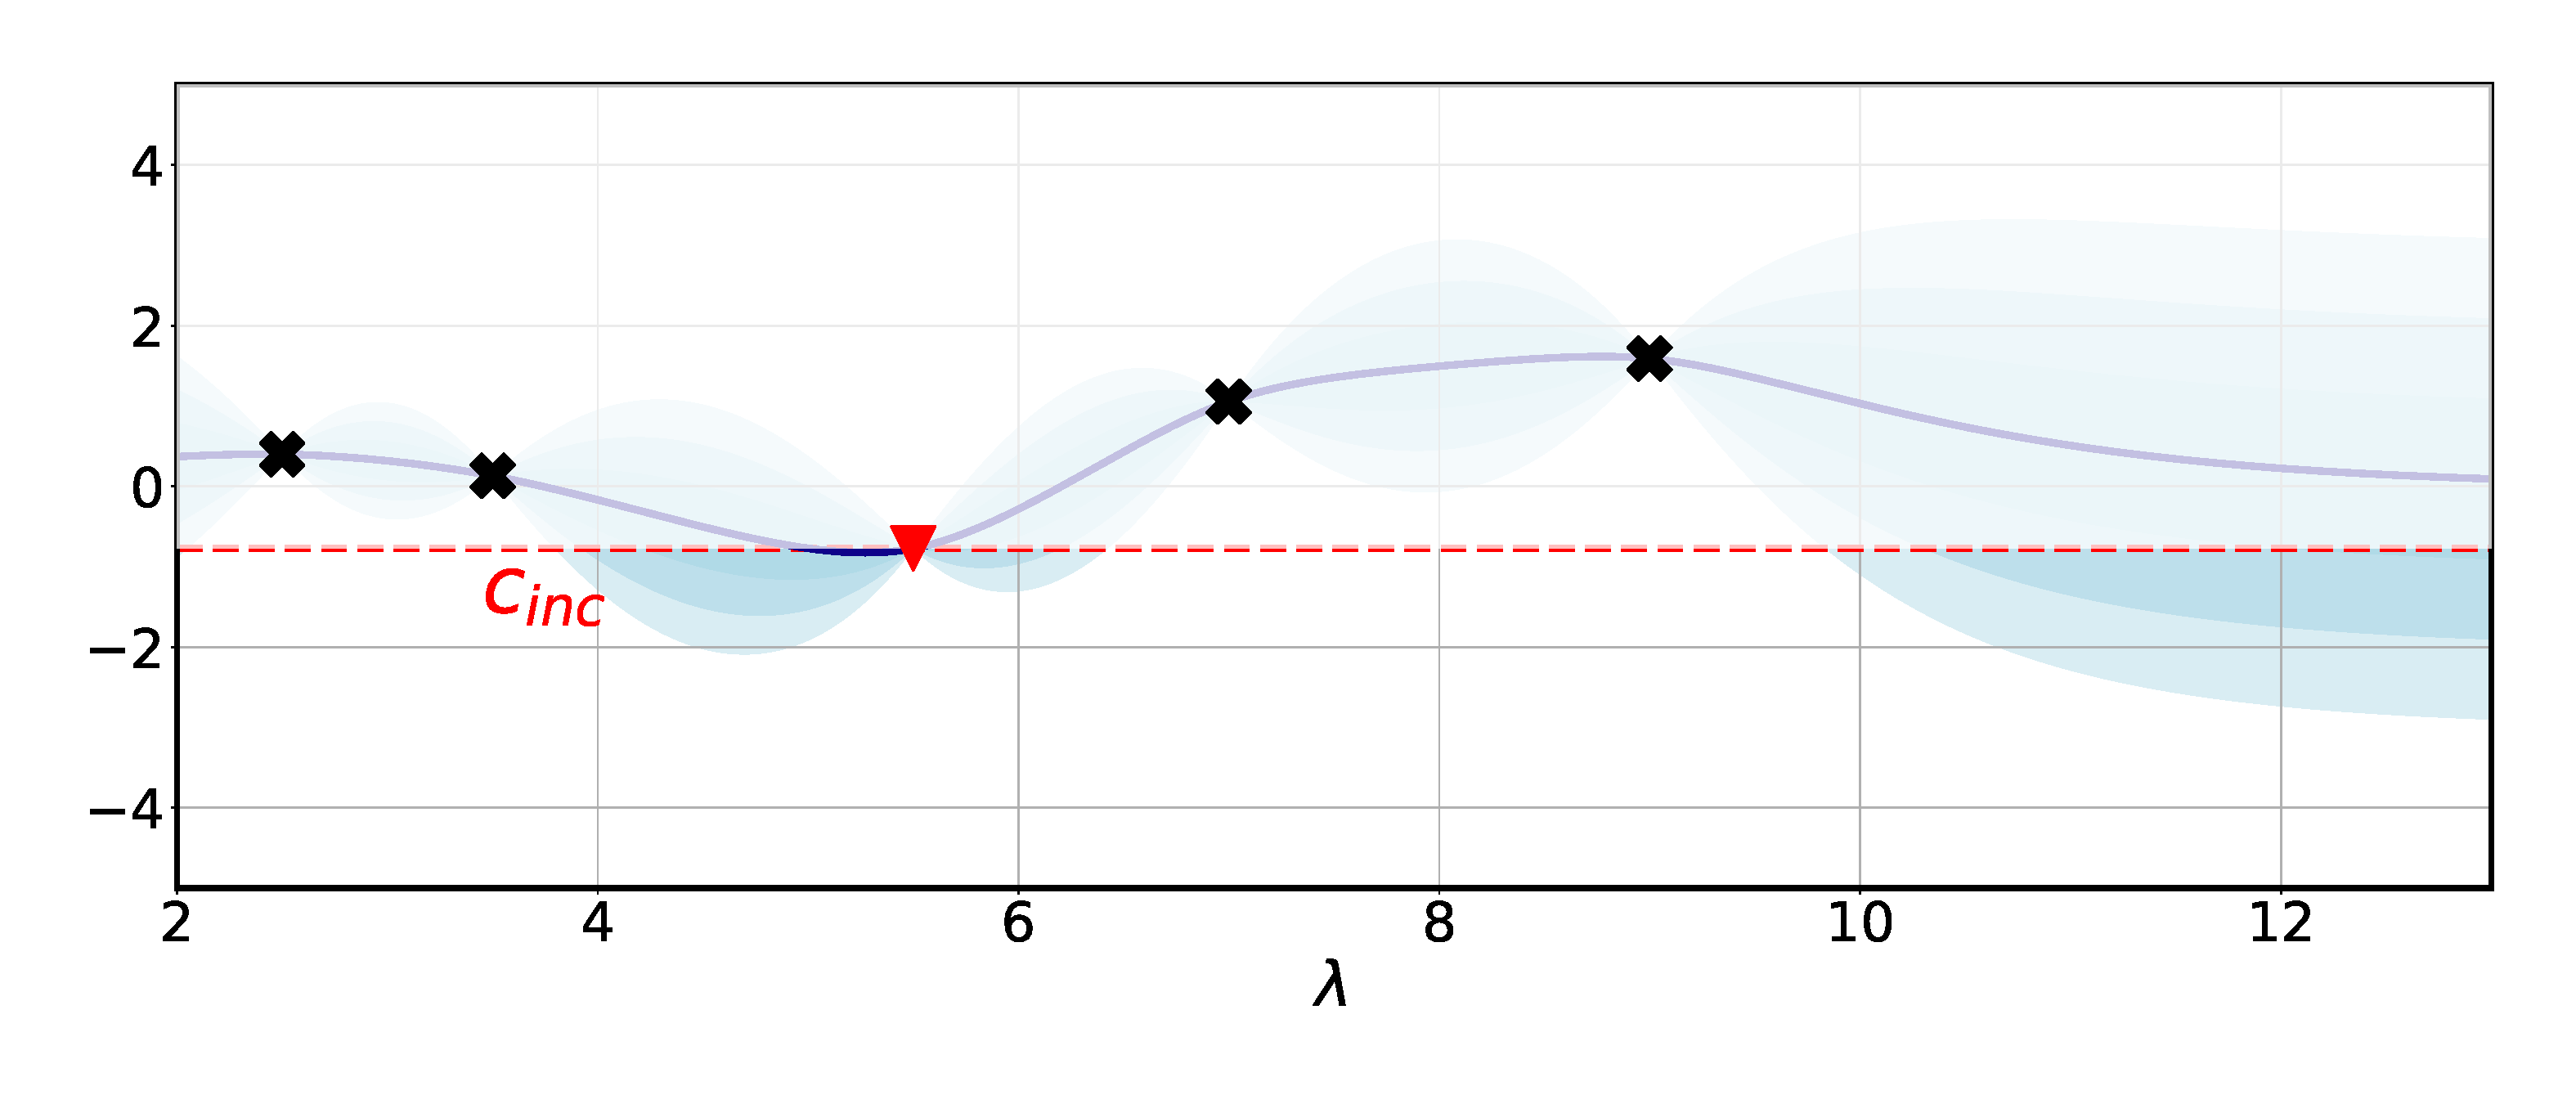
\includegraphics[width=\linewidth, height=0.7\textheight, keepaspectratio=true]{images/acq_func_images/pi/pi_4.pdf}};
        \node<.> [below=-1.0\belowcaptionskip of img4, align=center]{Intuitively, we care about the probability of improving over the current incumbent};
        \comment{We cannot be absolutely certain if there will be an improvement, but we are certain that if there is to be improvement, it is only possible in this zone.}
    
        \node<+> (img5) {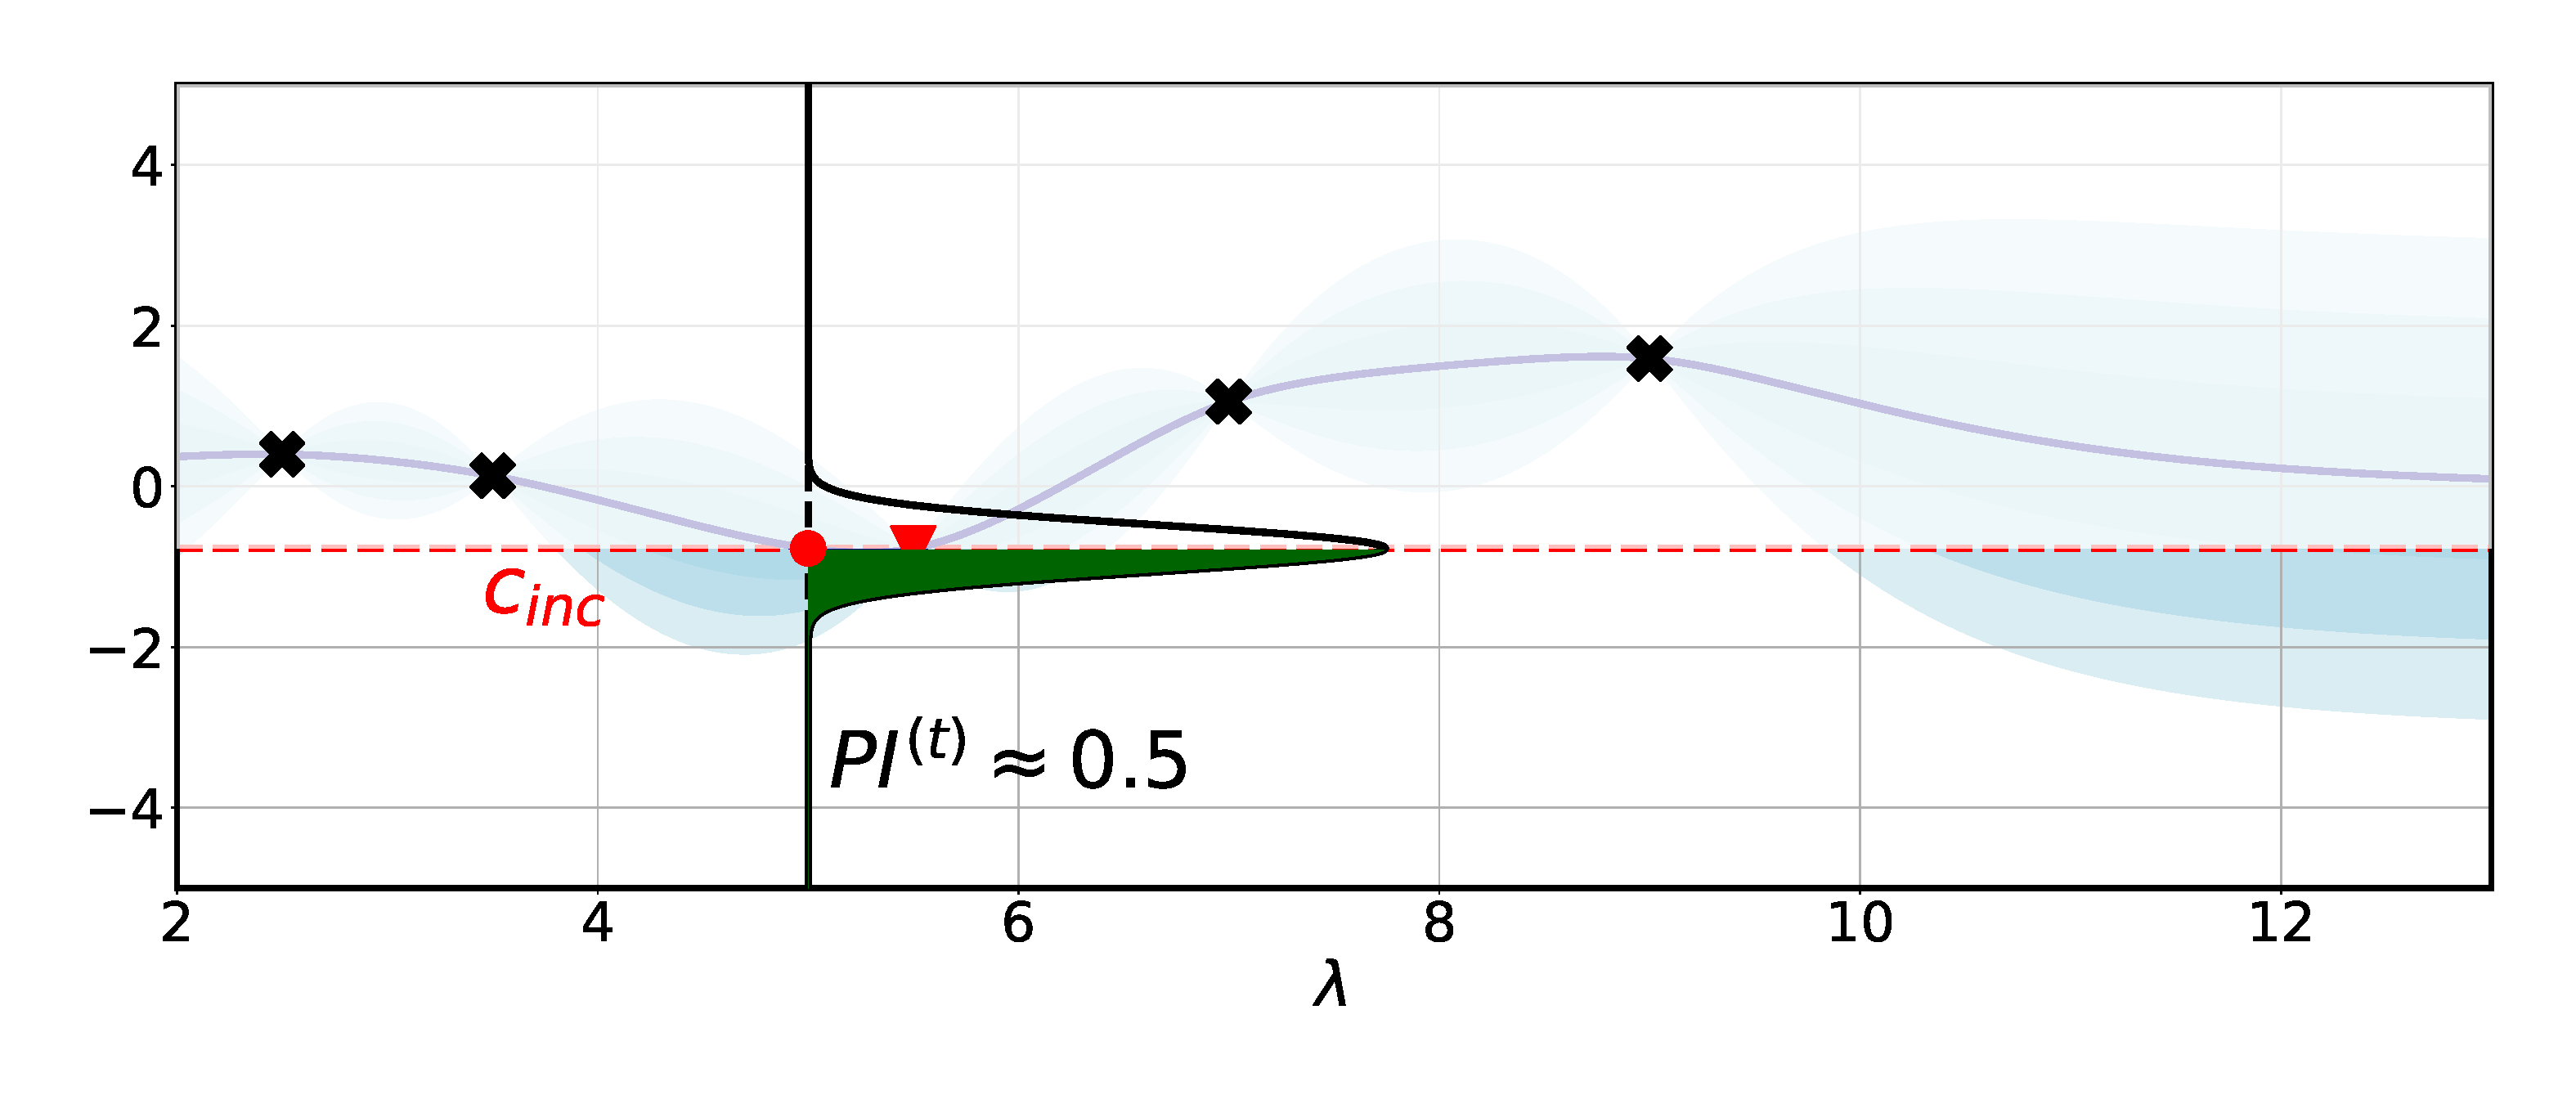
\includegraphics[width=\linewidth, height=0.7\textheight, keepaspectratio=true]{images/acq_func_images/pi/pi_5.pdf}};
        \node<.> [below=0.01\belowcaptionskip of img5, align=center]{PDF of a good candidate configuration. Only the green area is an improvement.};
    
        \node<+> (img6) {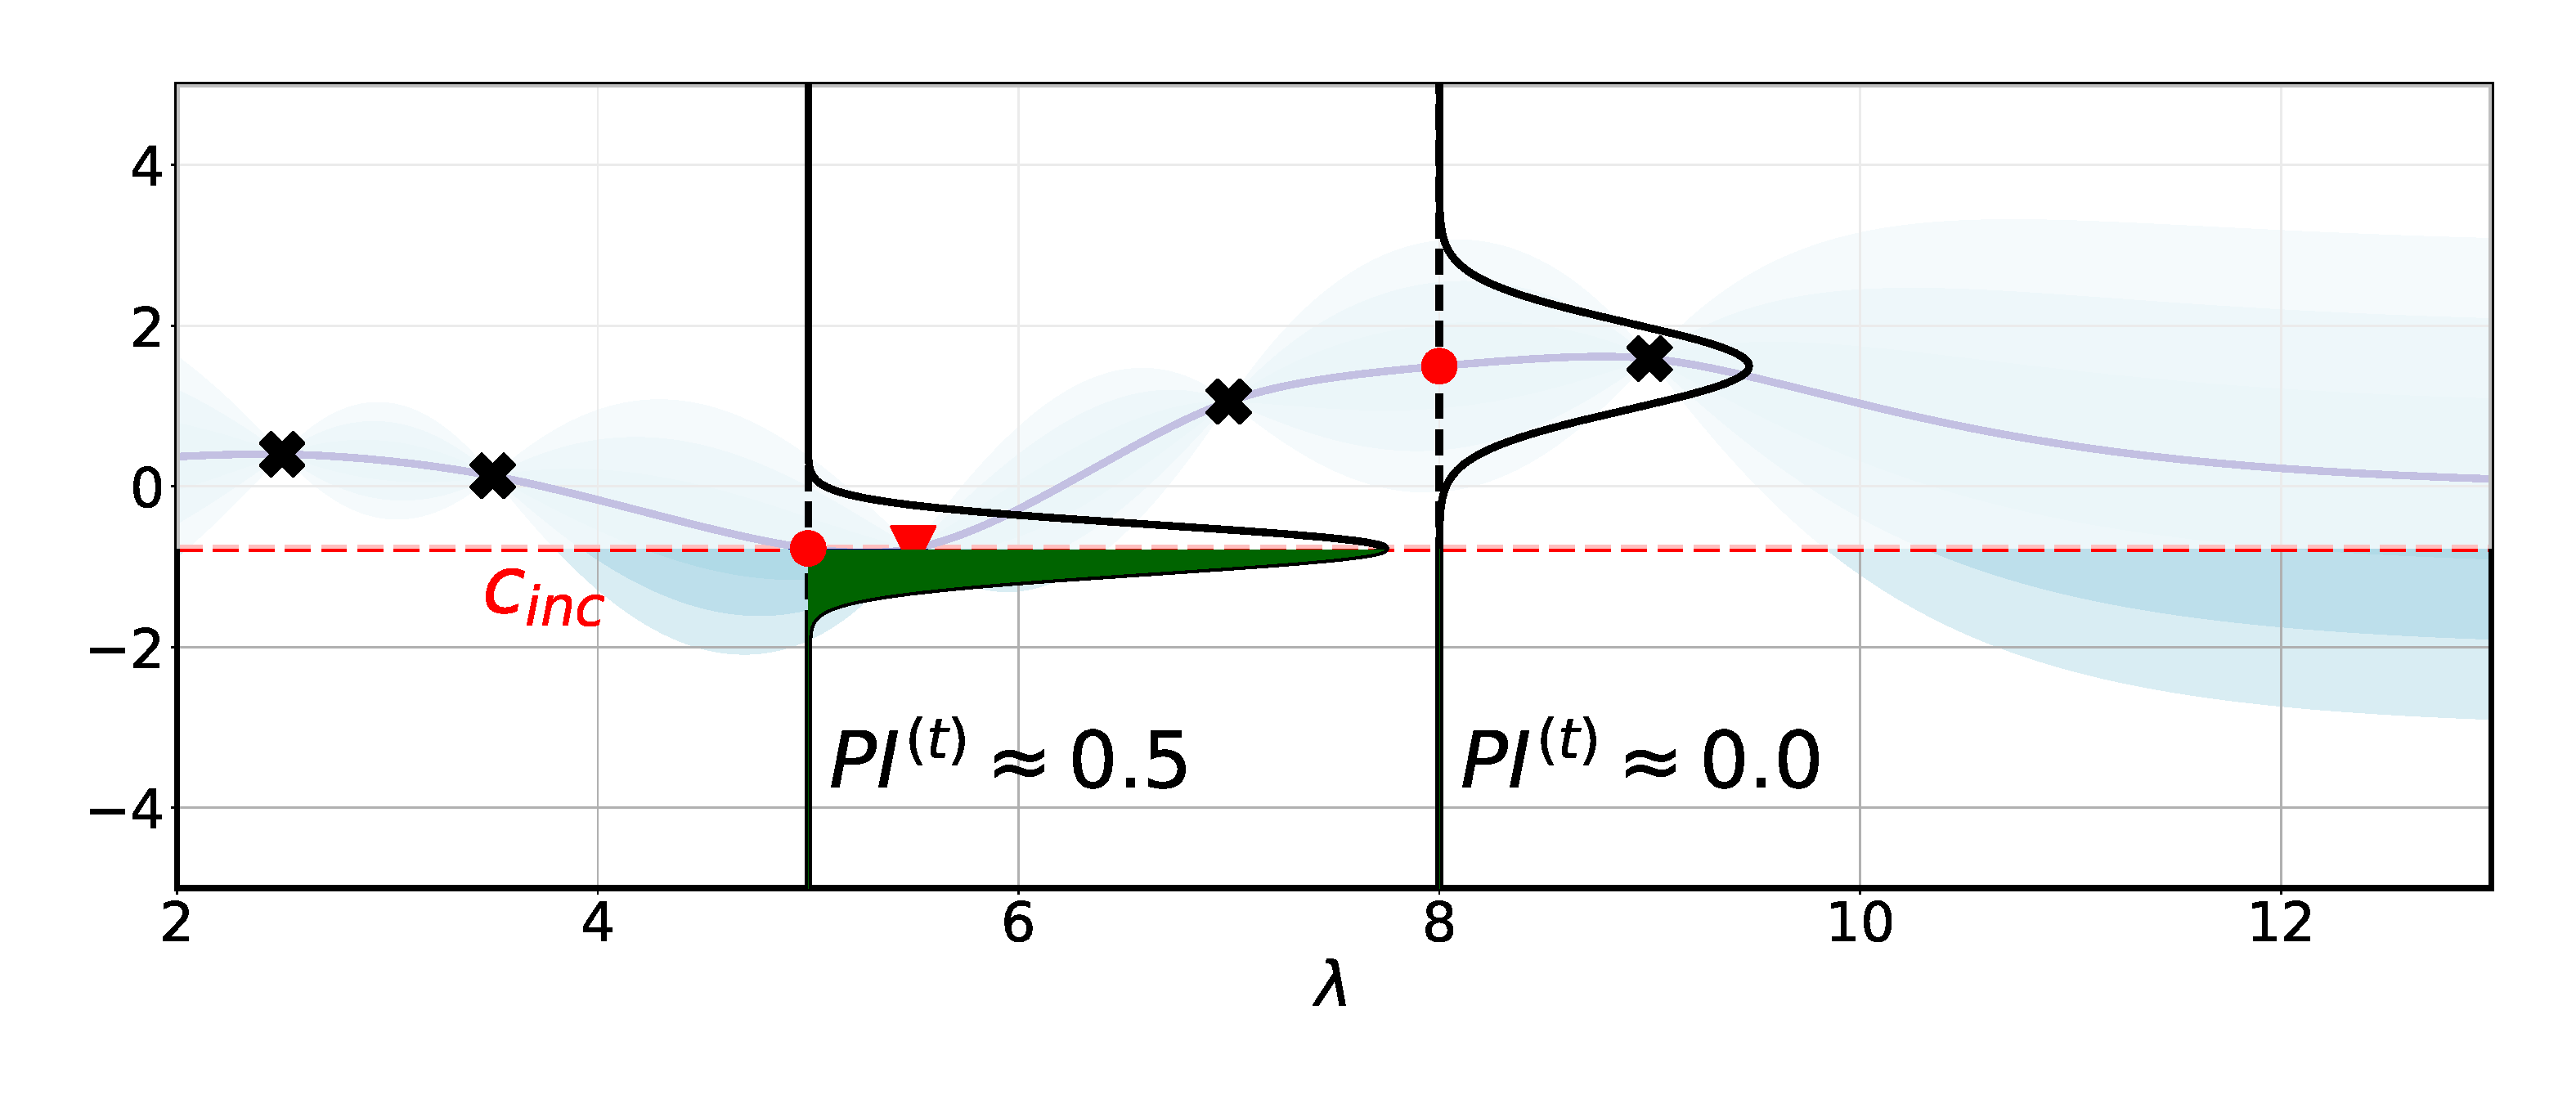
\includegraphics[width=\linewidth, height=0.7\textheight, keepaspectratio=true]{images/acq_func_images/pi/pi_6.pdf}};
        \node<.> [below=0.01\belowcaptionskip of img6, align=center]{PDF of a bad candidate configuration};
      \end{tikzpicture}
    % \end{figure}
    
}
\end{frame} 
% -----------------------------------------------------------------------
\begin{frame}[c]{Probability of Improvement (PI): Formal Definition}
%\framesubtitle{Probability of Improvement - Choosing a candidate}
%\comment{The definitions were adapted from the source to fit an acquisition function that is maximized and an objective function which is to be minimized.!}
\begin{itemize}
    \item We define the \alert{current incumbent at time step $t$} as: 
    $\incumbent[\bocount-1]\in\argmin_{\conf'\in\iter[\bocount-1]{\dataset}}\obs[\conf']$
    \item We write \alert{$\cost_{inc}$} shorthand for the \alert{cost of the current incumbent}: 
    $c_{inc} = \cost(\incumbent[\bocount-1])$
\smallskip
        \item The \alert{probability of improvement $\acq_{PI}(\conf)$} at a configuration $\conf$ is then defined as: 
        \alert{\[\iter{\acq}_{PI}(\conf) = P(\cost(\conf) \leq \cost_{inc}).\]}
    \vspace*{-0.5cm}
    \pause
    \item Since the predictive distribution for $\cost(\conf)$ is a Gaussian $\normaldist(\iter[\bocount-1]{\mean}(\conf), \iter[\bocount-1]{\variance}(\conf))$, this can be written as:
    \[
        \alert{\iter{\acq}_{PI}(\conf) = \cdf[Z]}, \quad \text{with } Z = \dfrac{\cost_{inc} - \iter[\bocount-1]{\mean}(\conf) - \xi}{\iter[\bocount-1]{\stddev}(\conf)}, 
    \]
    \newline
    where $\cdf(\cdot)$ is the CDF of the standard normal distribution and $\xi$ is an optional exploration parameter
    \pause
    \item[] \[\boxed{\text{Choose}\;\;\bonextsample \in \argmax_{\conf\in\pcs}(\iter{\acq}_{PI}(\conf))}\]
%    \comment{Source: Tutorial by Brochu et al.: https://arxiv.org/pdf/1012.2599.pdf }
\end{itemize}
\end{frame}
%-----------------------------------------------------------------------
\begin{frame}[t]{Expected Improvement (EI): Concept}
%\framesubtitle{Expected Improvement - Concept}

% \begin{figure}
  \centering
  \begin{tikzpicture}
    \node<+> (img1) {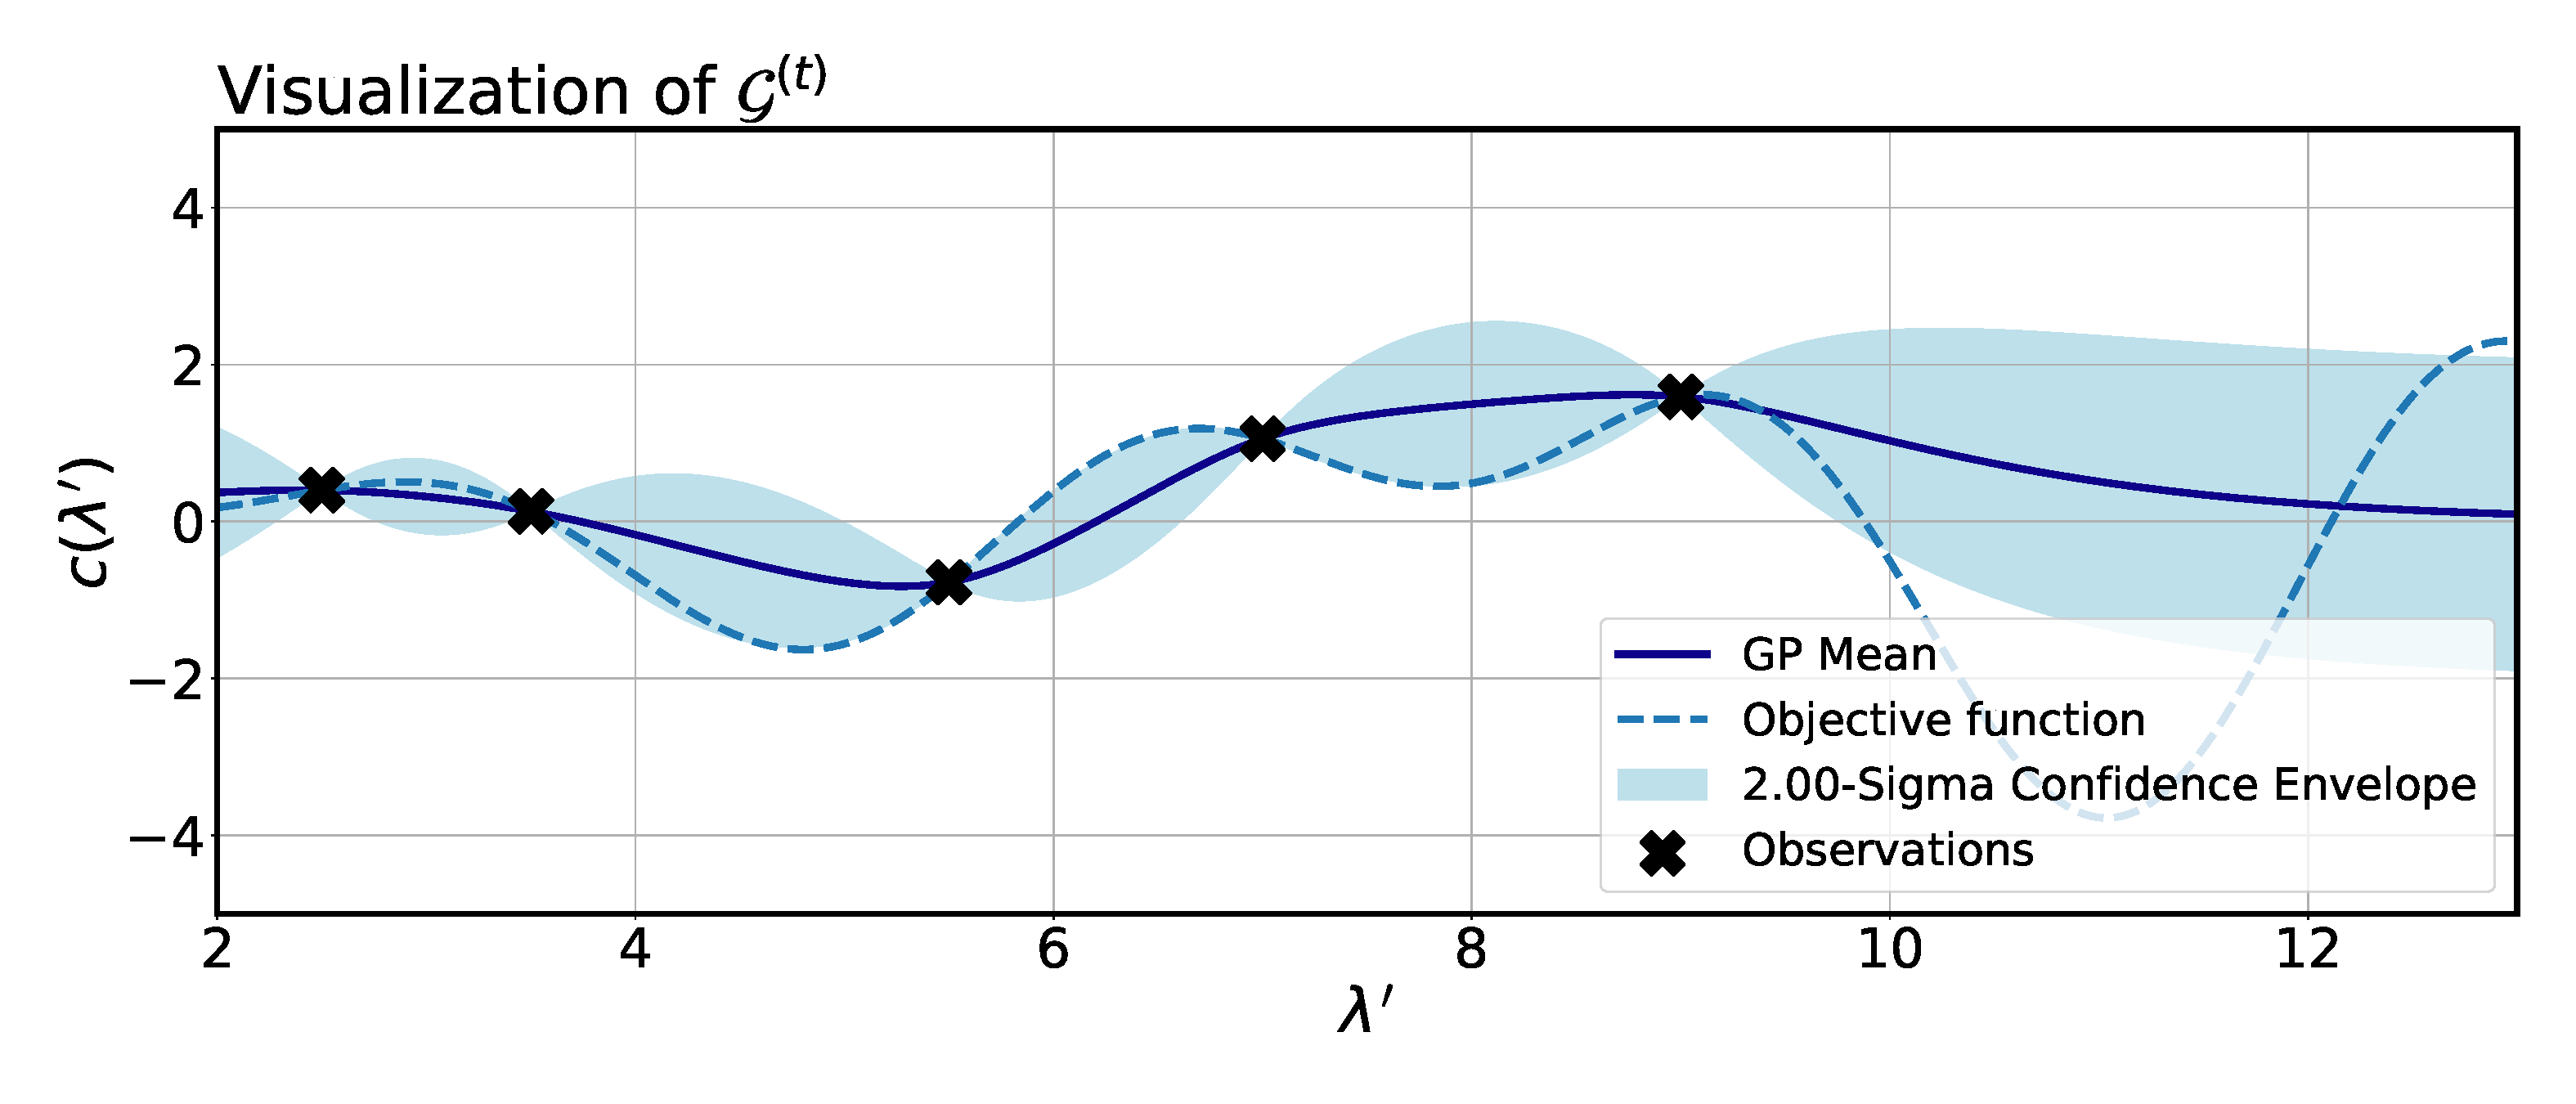
\includegraphics[width=\linewidth, height=0.7\textheight, keepaspectratio=true]{images/acq_func_images/ei/ei_1.pdf}};
    \node<.> [below=0.01\belowcaptionskip of img1, align=center]{Given the surrogate fit at iteration $\bocount$};

    \node<+> (img2a) {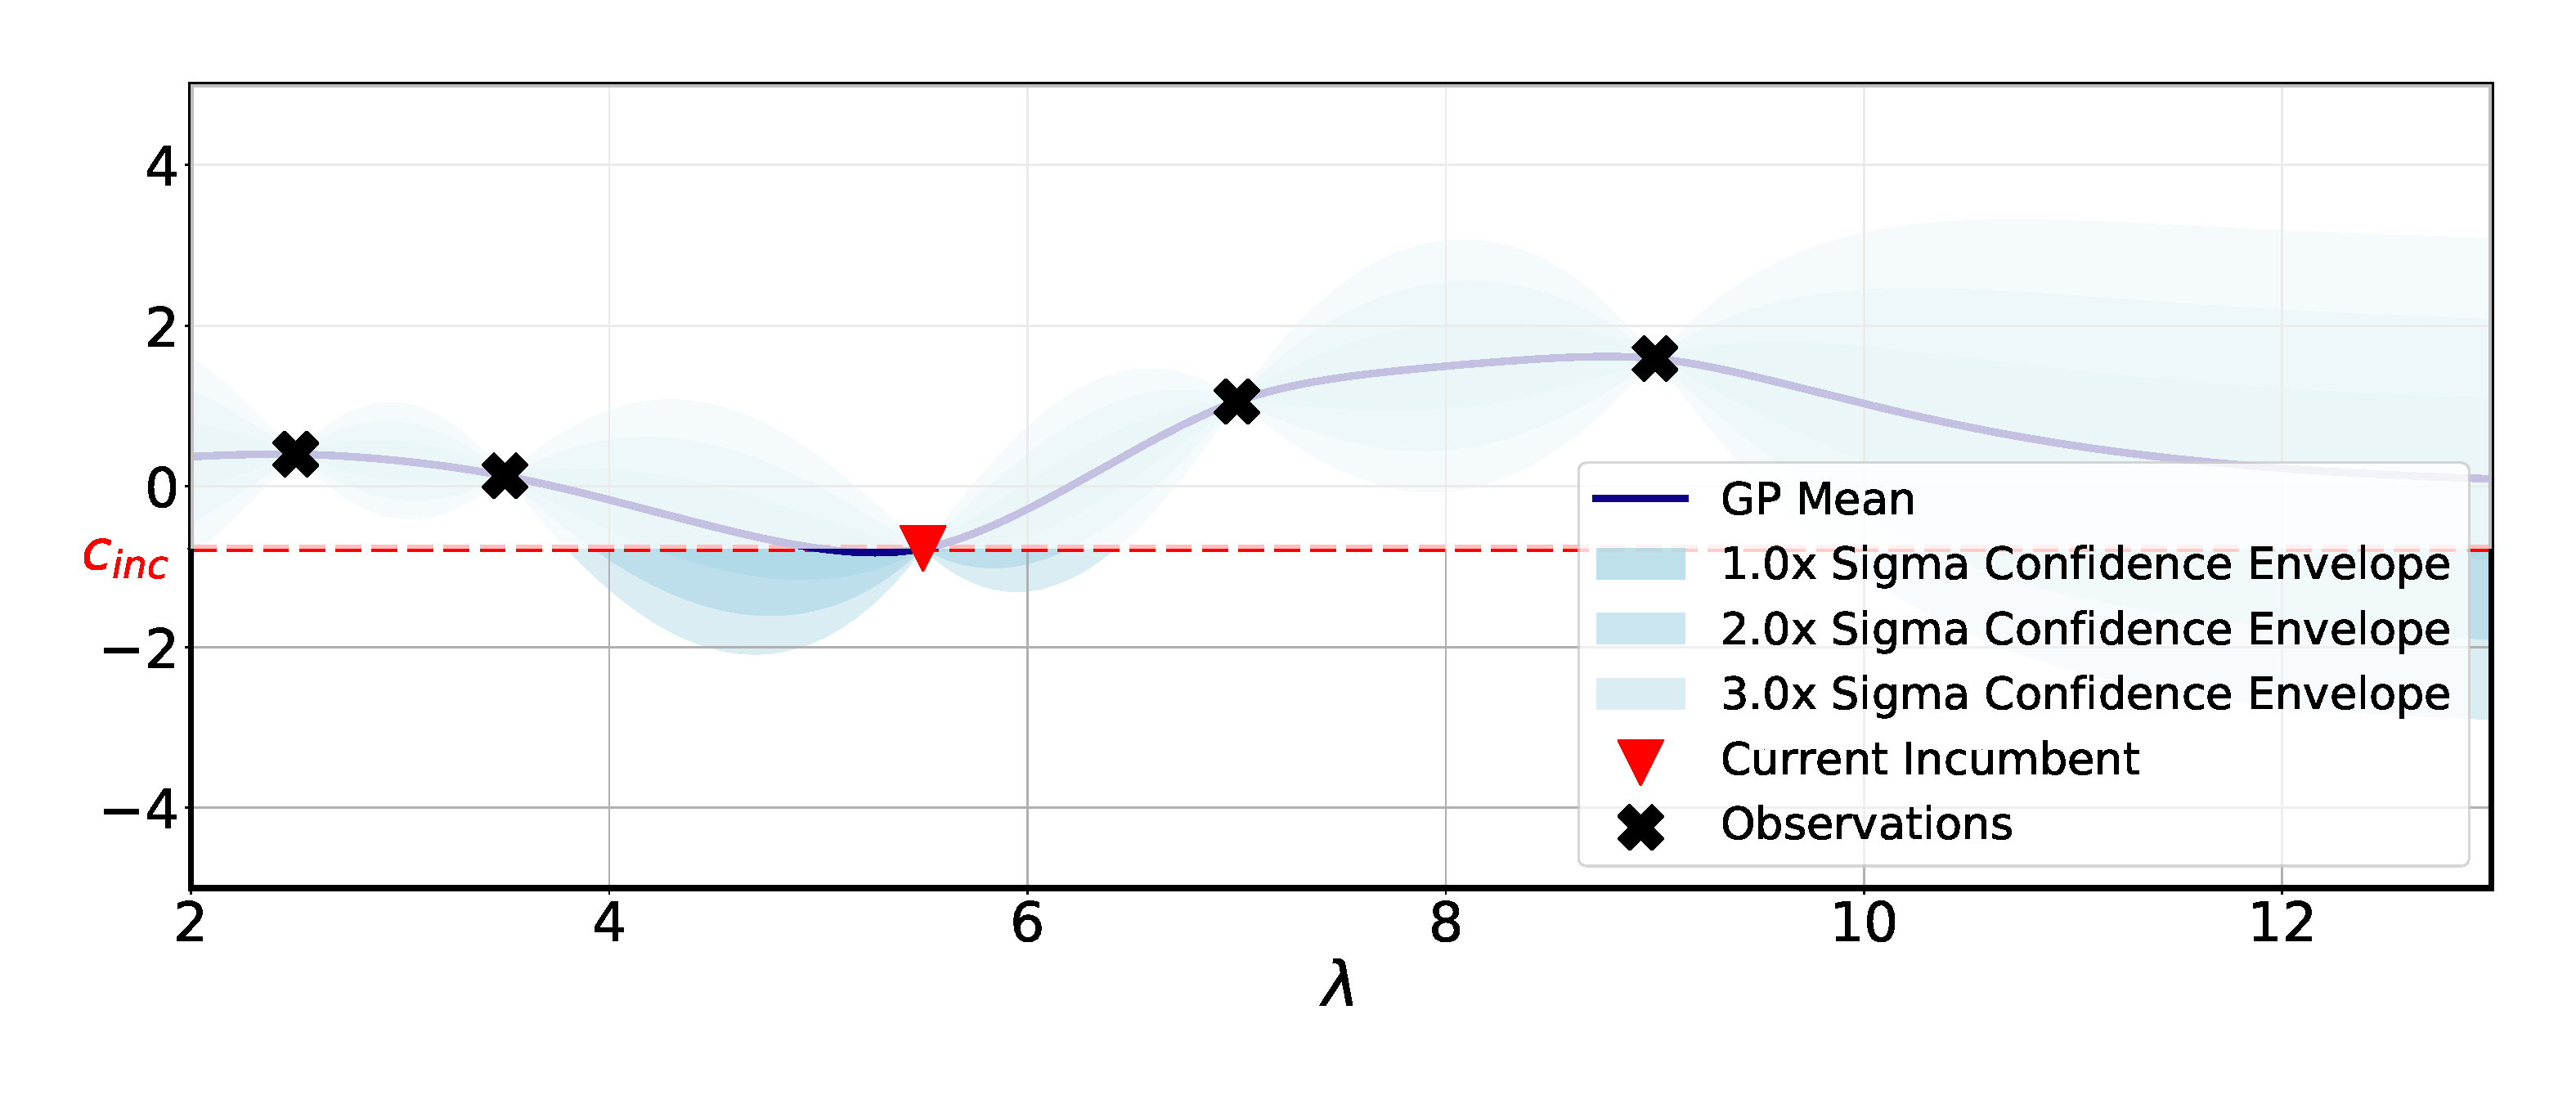
\includegraphics[width=\linewidth, height=0.7\textheight, keepaspectratio=true]{images/acq_func_images/ei/ei_2a.pdf}};
    \node<.> [below=0.01\belowcaptionskip of img2a, align=center]{Region of probable improvement -- but \alert{how large} is the improvement?};

    \node<+> (img2b) {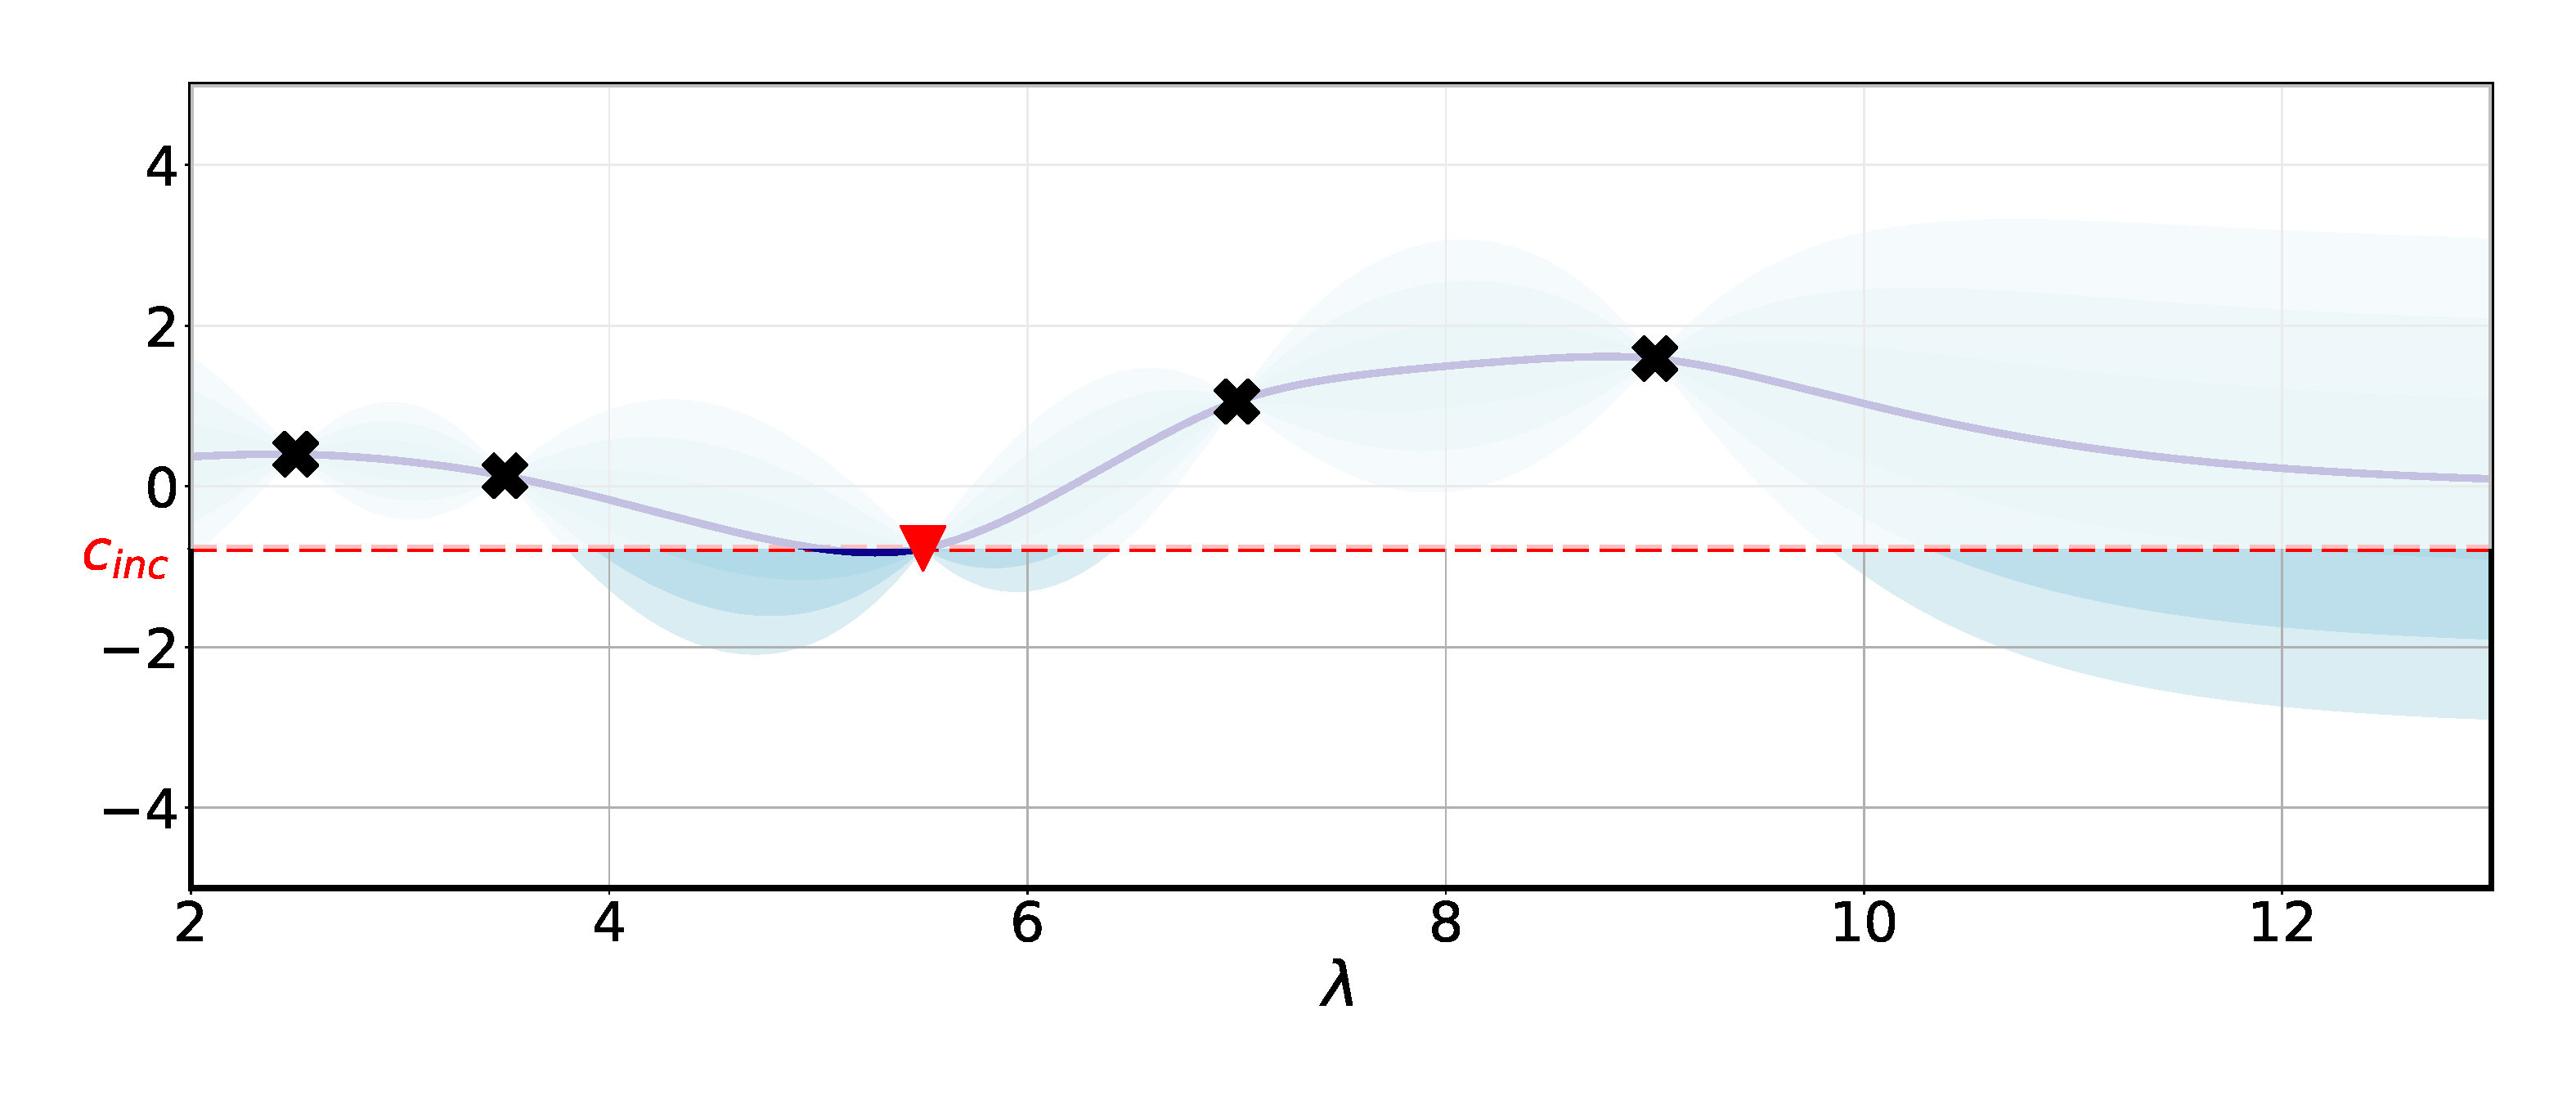
\includegraphics[width=\linewidth, height=0.7\textheight, keepaspectratio=true]{images/acq_func_images/ei/ei_2b.pdf}};
    \node<.> [below=0.01\belowcaptionskip of img2b, align=center]{Region of probable improvement -- but \alert{how large} is the improvement?};

    \node<+> (img3) {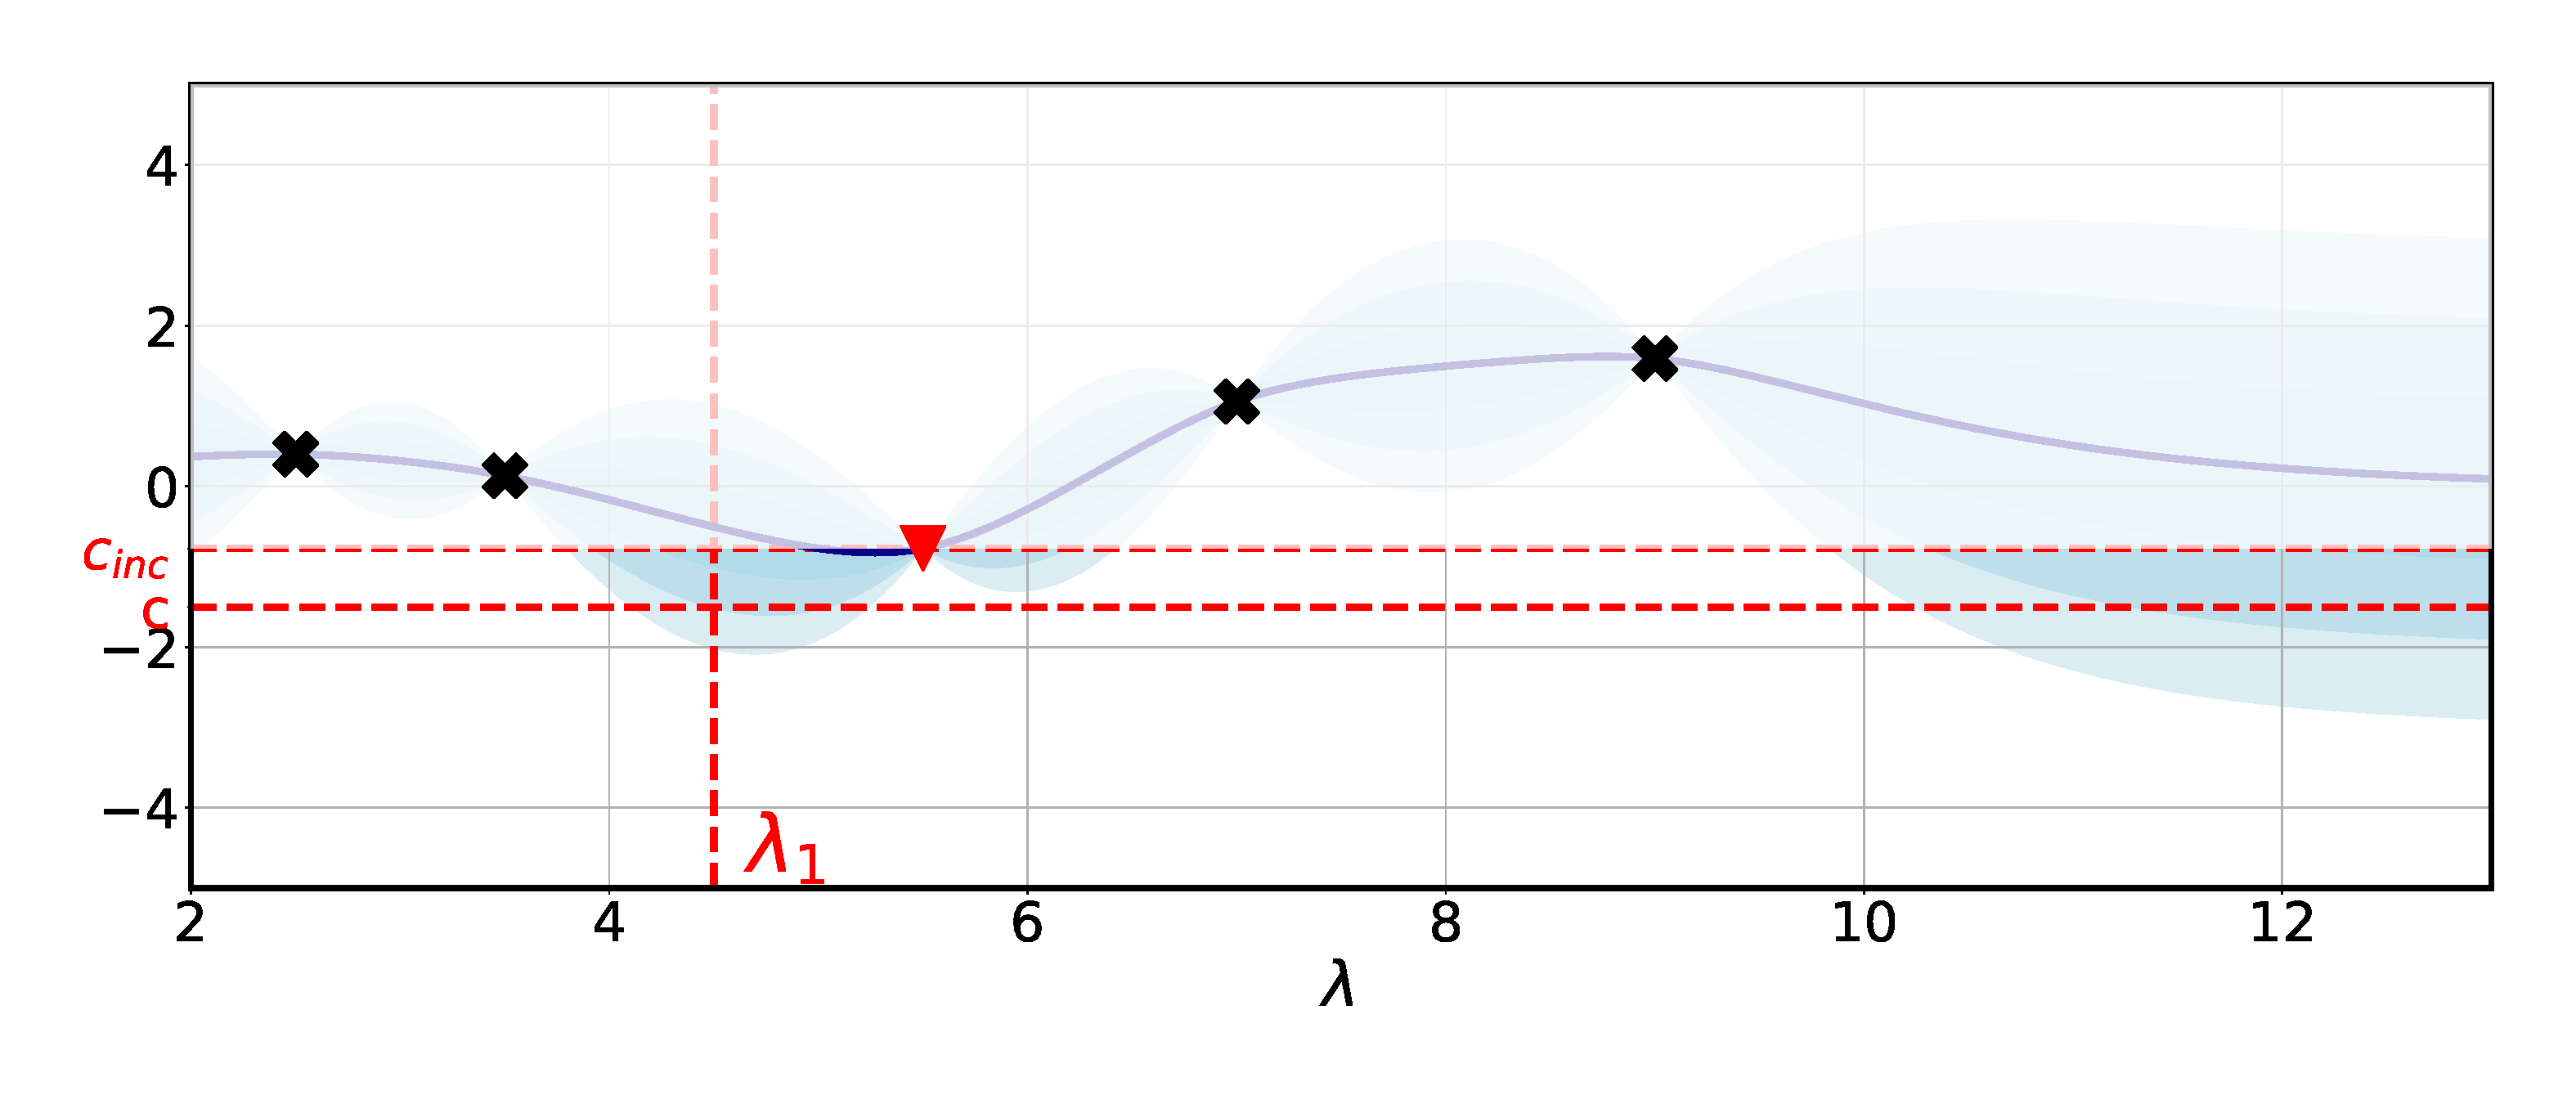
\includegraphics[width=\linewidth, height=0.7\textheight, keepaspectratio=true]{images/acq_func_images/ei/ei_3.pdf}};
    \node<.> [below=0.01\belowcaptionskip of img3, align=center]{Hypothetical \emph{real} cost $c$ at a given $\conf$ - unknown in practice without evaluating};

    \node<+> (img4) {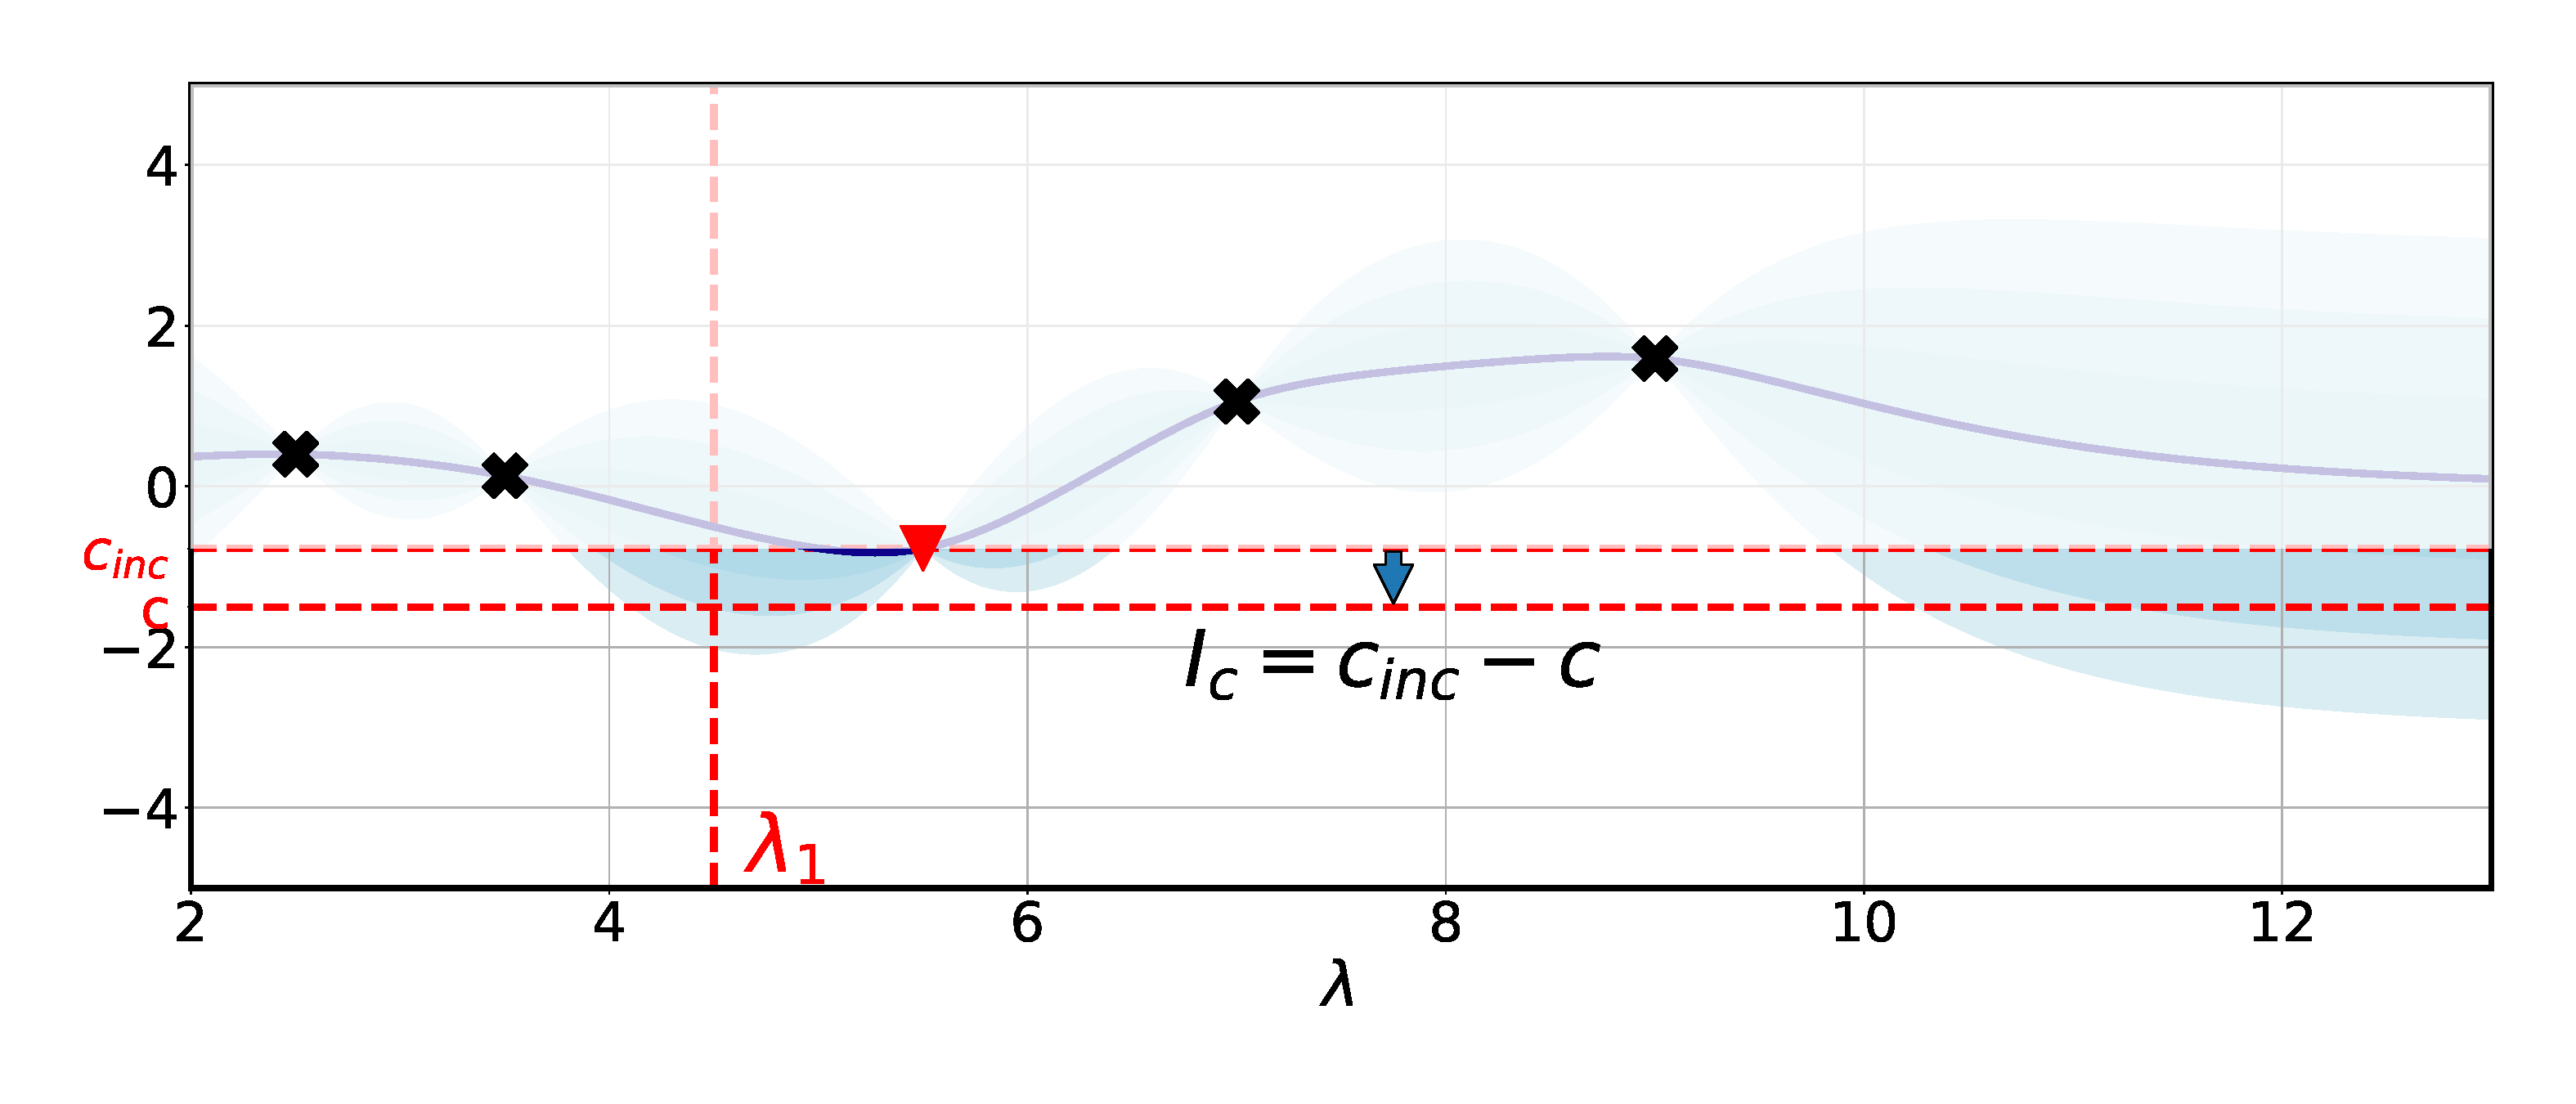
\includegraphics[width=\linewidth, height=0.7\textheight, keepaspectratio=true]{images/acq_func_images/ei/ei_4.pdf}};
    \node<.> [below=-0.01\belowcaptionskip of img4, align=center]{Given a hypothetical $c$, we can compute the improvement $I_c(\conf)$};
%    Without performing an actual evaluation, we cannot calculate $\iter{I}(\conf)$};

    \node<+> (img5) {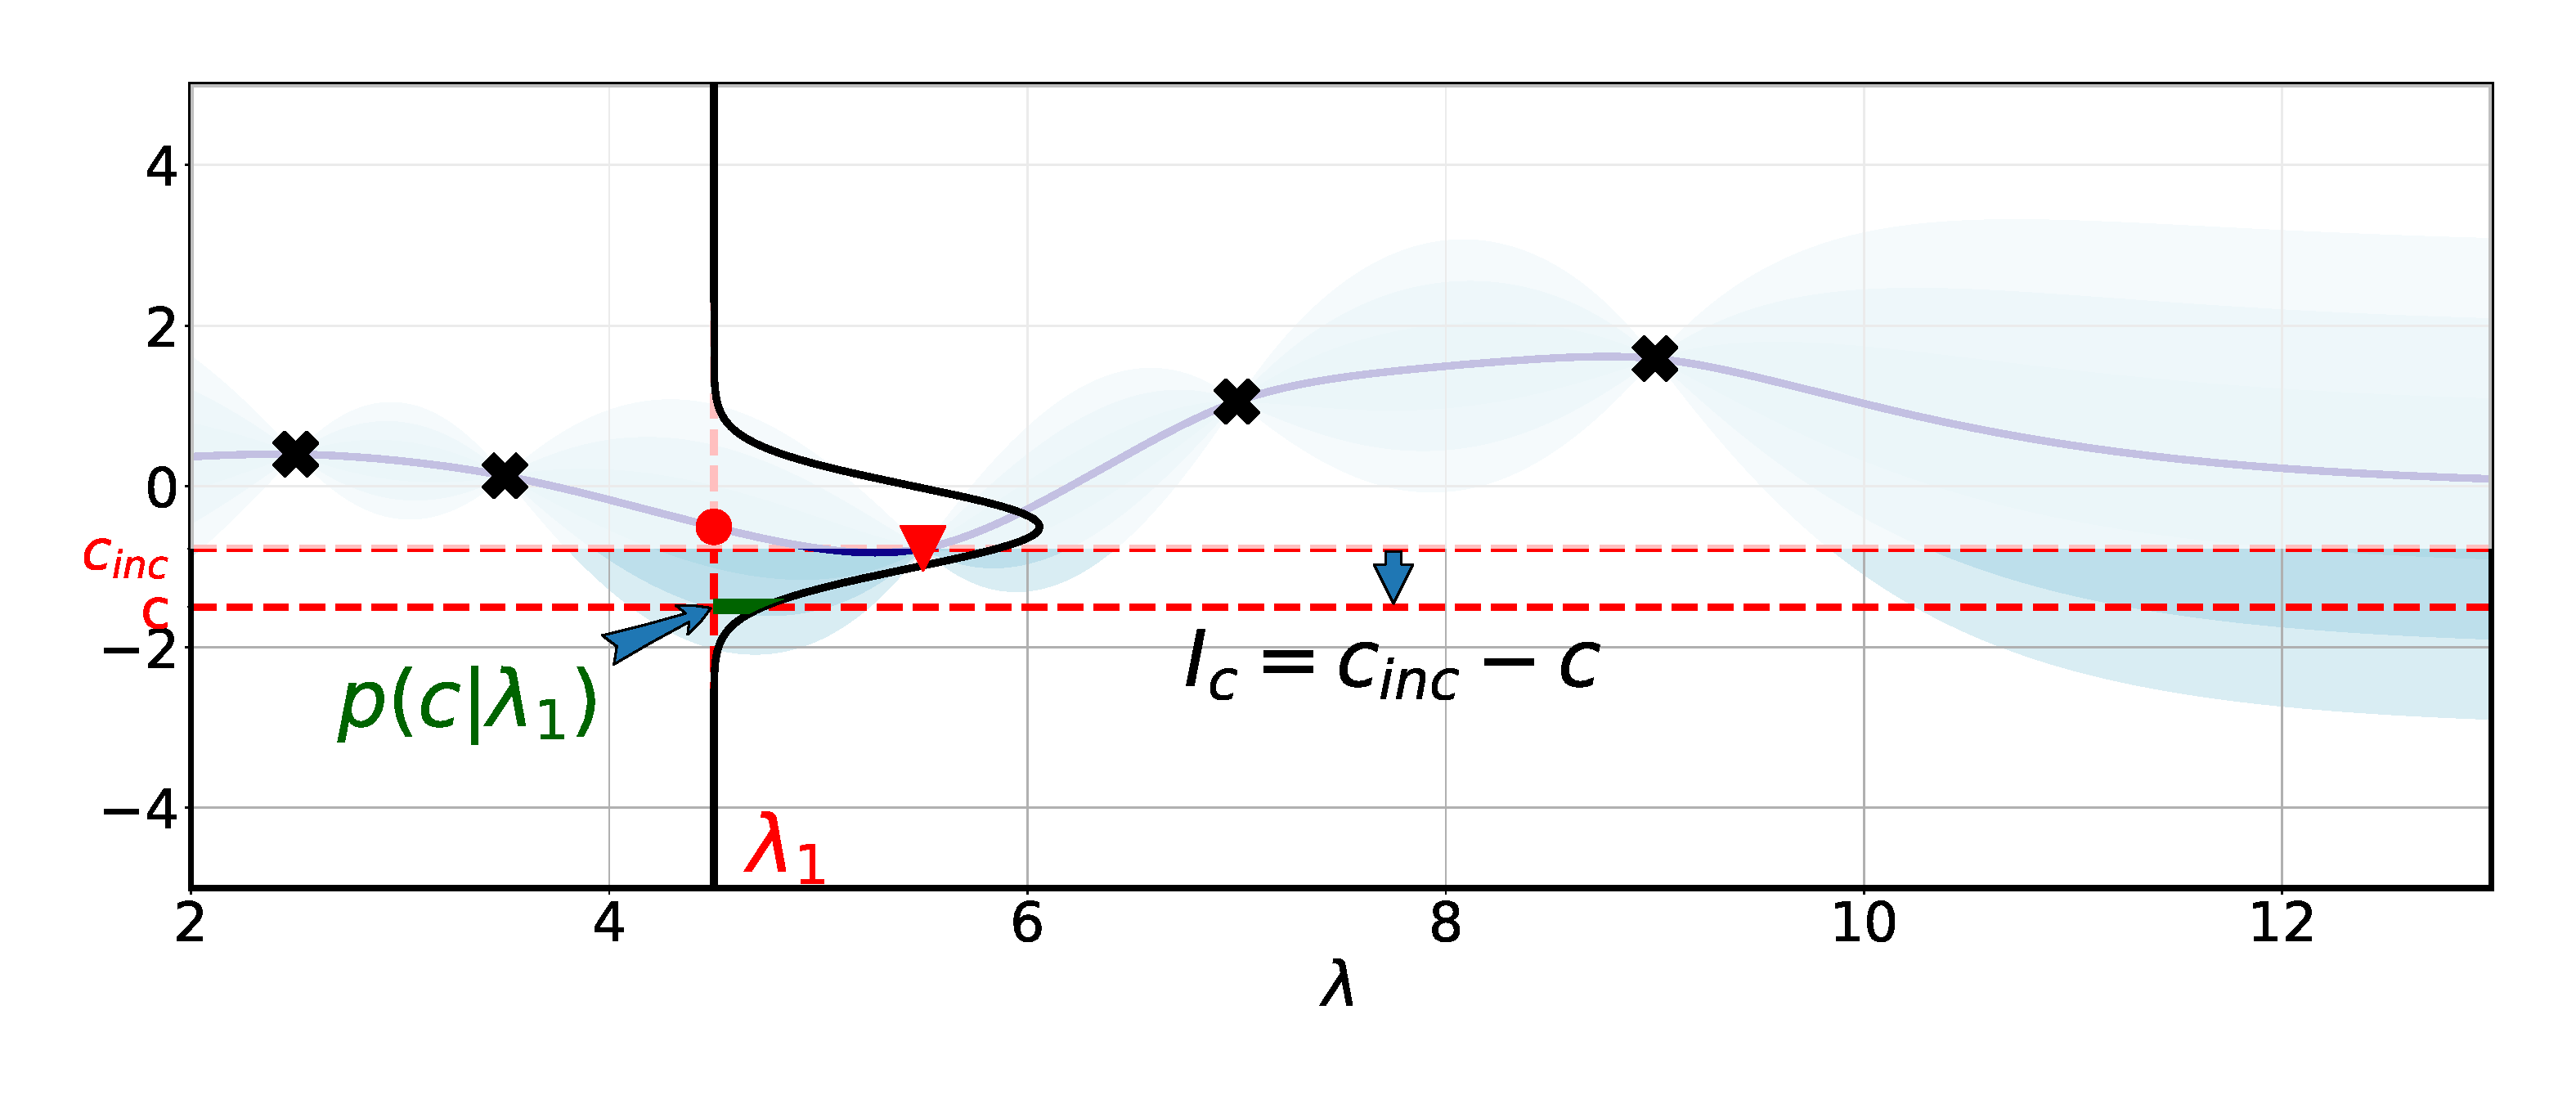
\includegraphics[width=\linewidth, height=0.7\textheight, keepaspectratio=true]{images/acq_func_images/ei/ei_5.pdf}};
    \node<.> [below=0.01\belowcaptionskip of img5, align=center]{Given $\surro(\conf) = \normaldist( \mean(\conf), \variance(\conf))$, we can also compute $p(\cost|\conf)$.};

    \node<+> (img6) {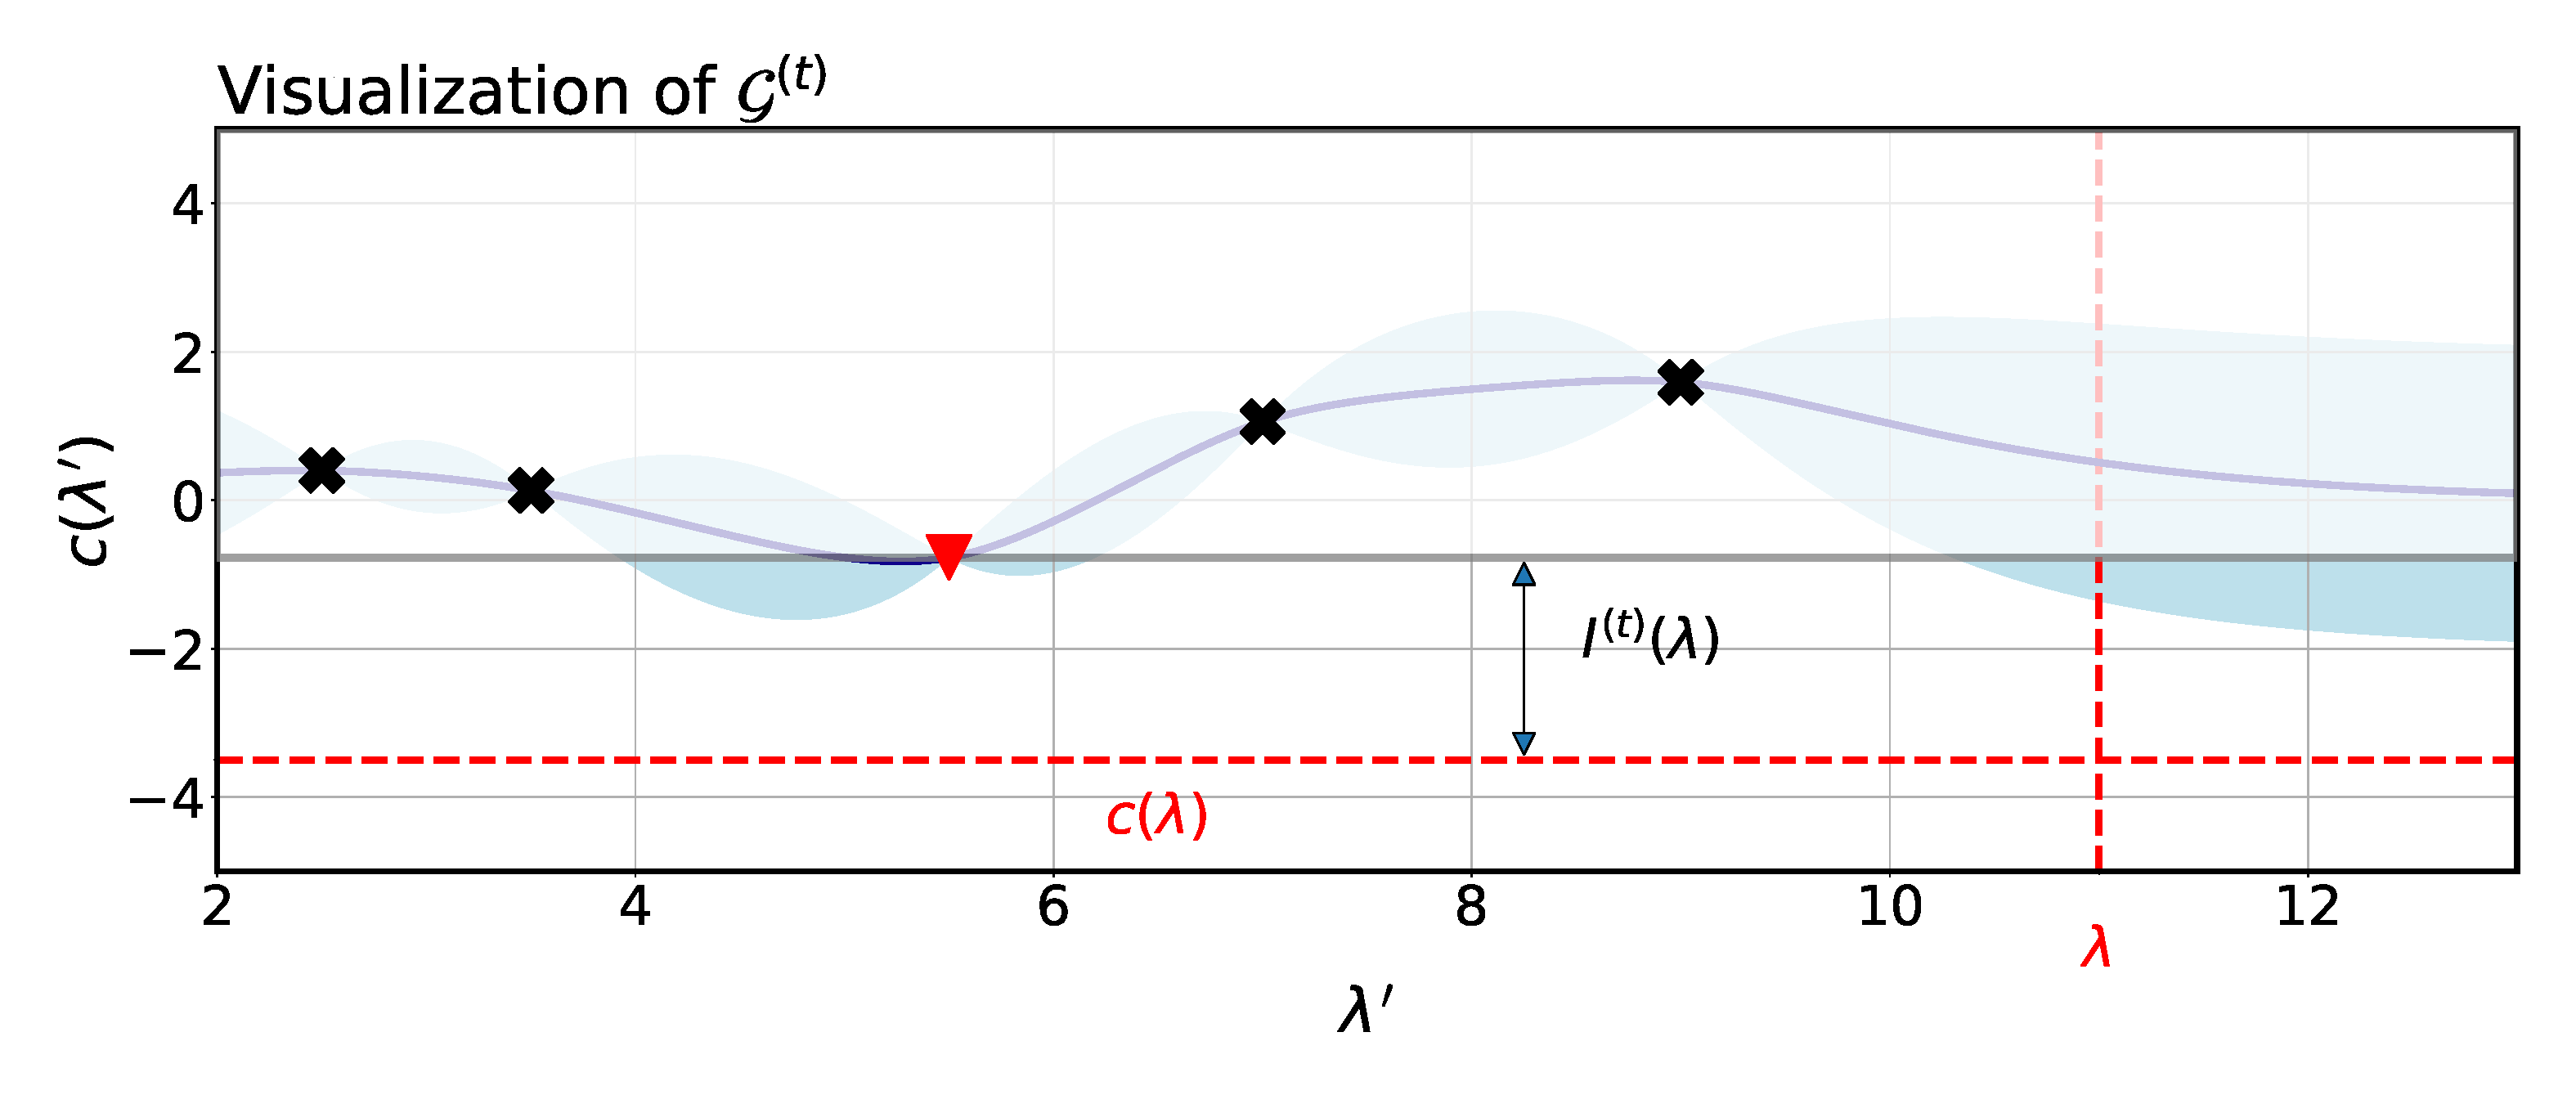
\includegraphics[width=\linewidth, height=0.7\textheight, keepaspectratio=true]{images/acq_func_images/ei/ei_6.pdf}};
    \node<.> [below=-0.01\belowcaptionskip of img6, align=center]{Compare the likelihood of a given improvement for two different configurations $\conf_1$ and $\conf_2$};

    \node<+> (img7) {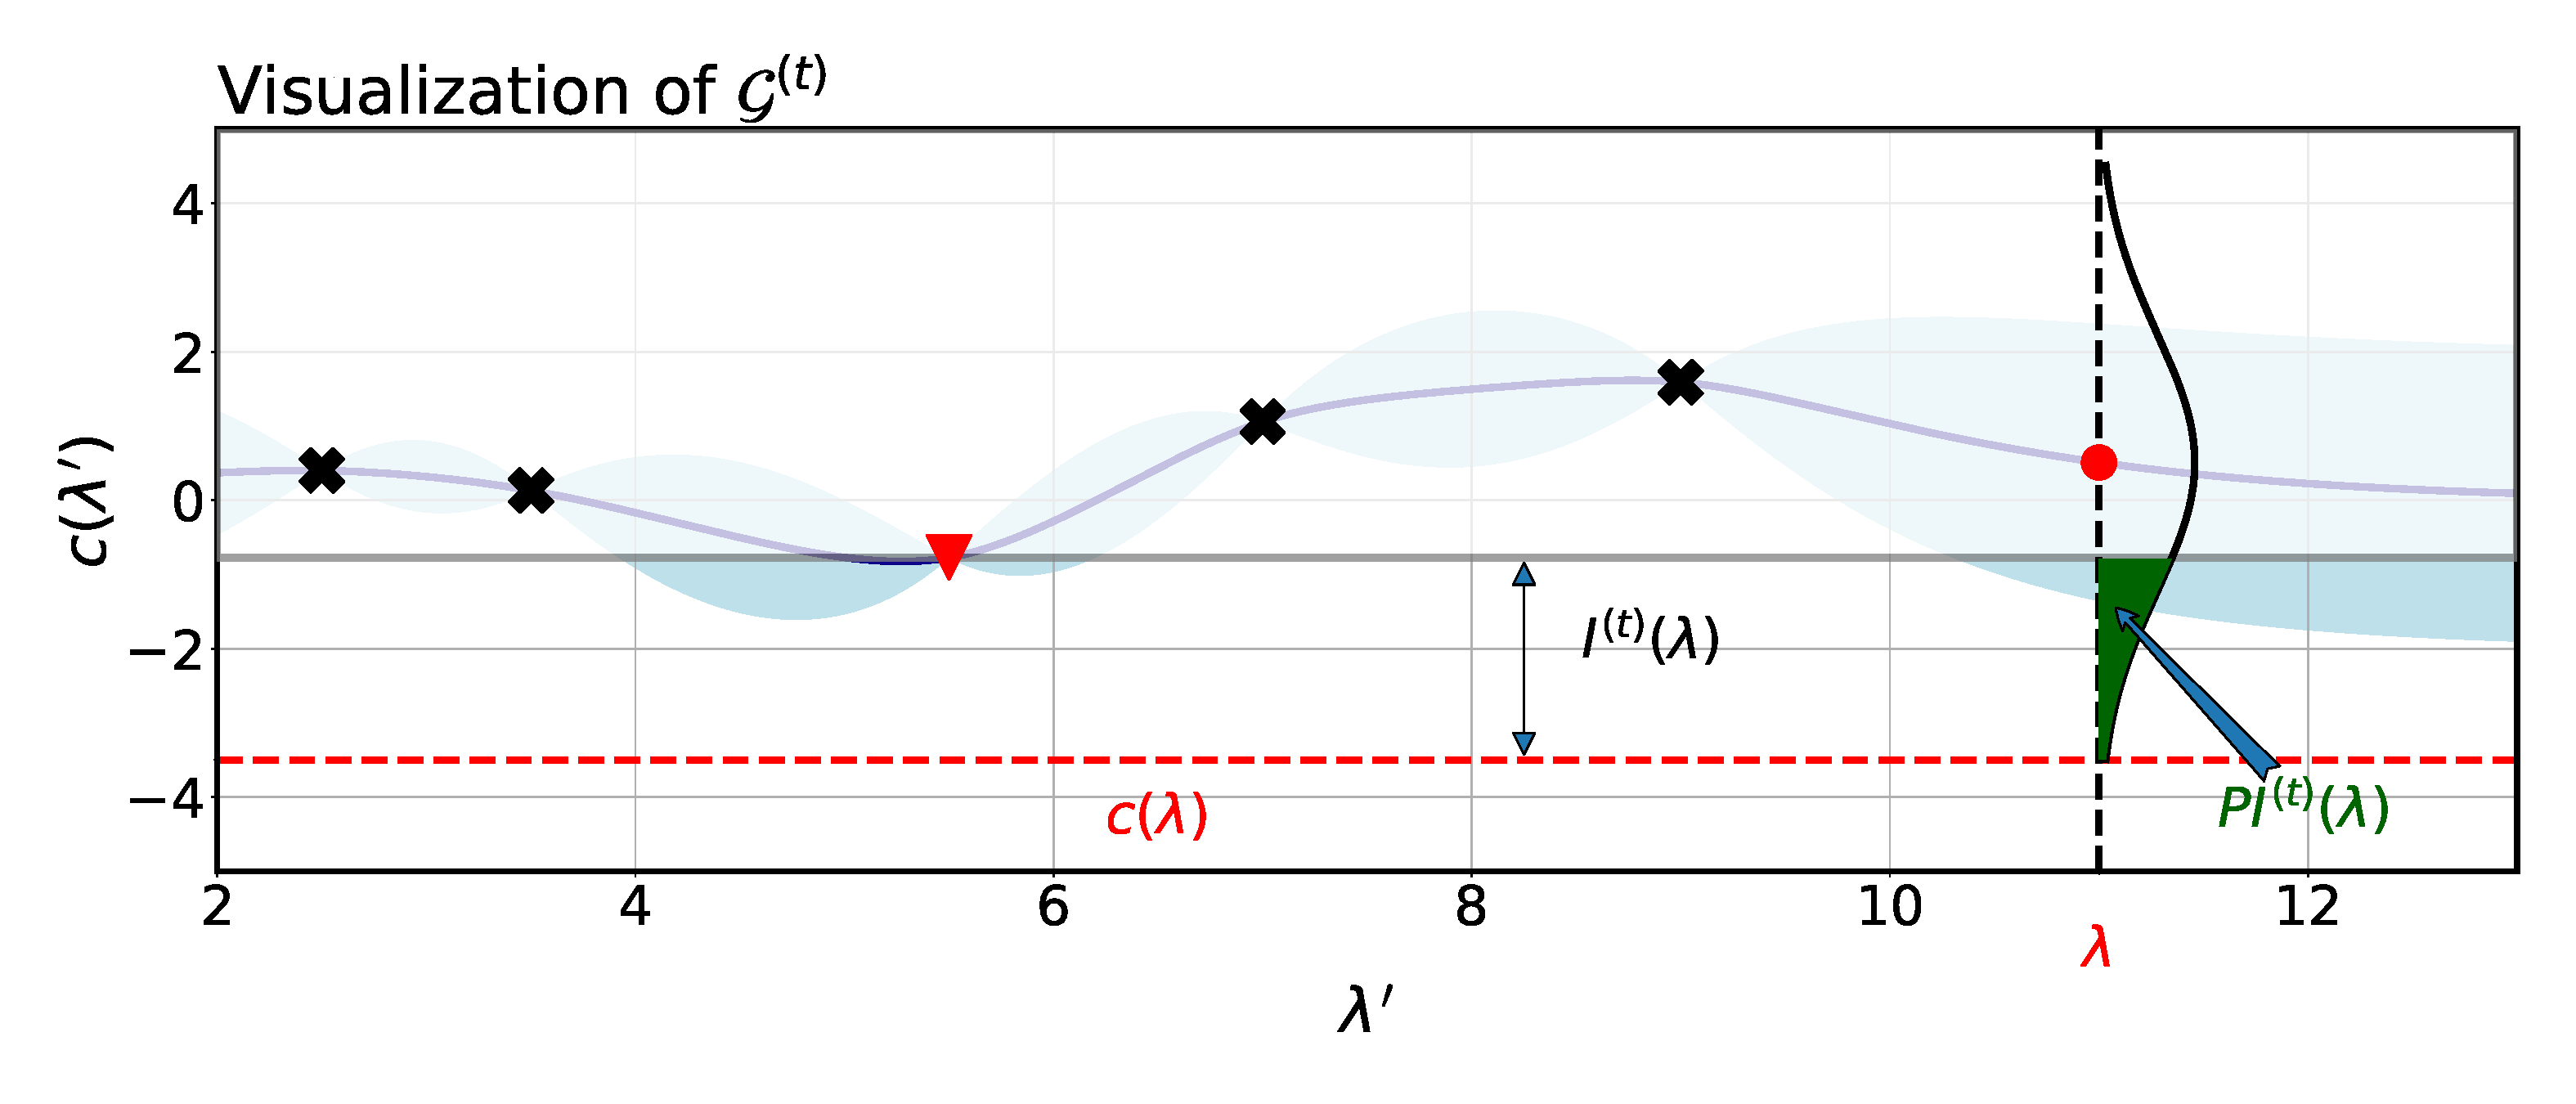
\includegraphics[width=\linewidth, height=0.7\textheight, keepaspectratio=true]{images/acq_func_images/ei/ei_7.pdf}};
    \node<.> [below=0.01\belowcaptionskip of img7, align=center]{Now consider the likelihood of a larger improvement.};
    
    \node<+> (img8) {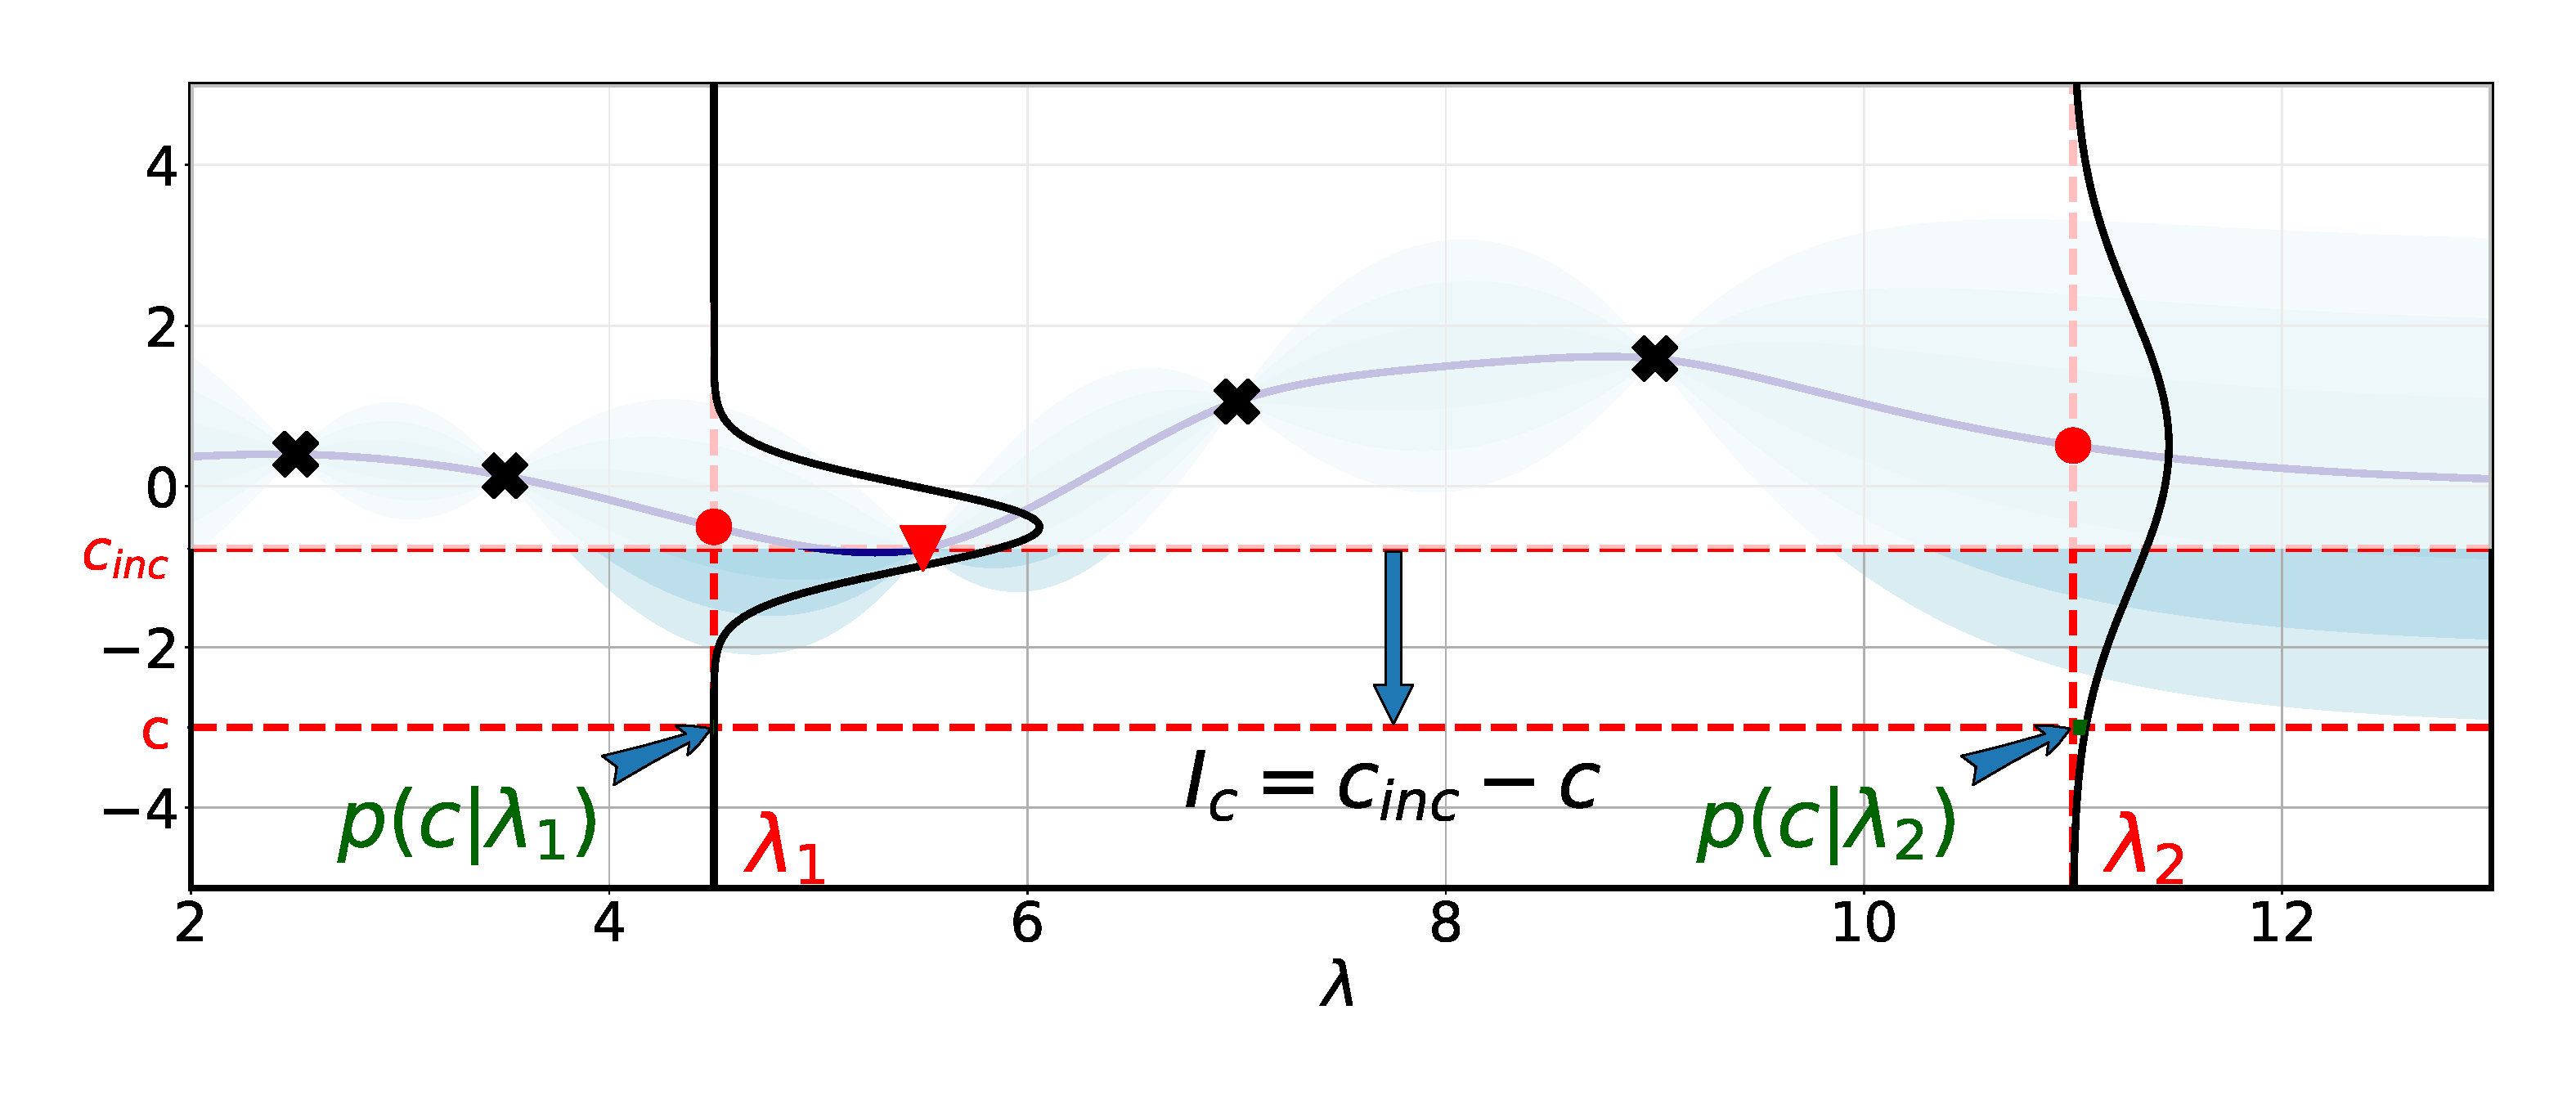
\includegraphics[width=\linewidth, height=0.7\textheight, keepaspectratio=true]{images/acq_func_images/ei/ei_8.pdf}};
    \node<.> [below=-0.01\belowcaptionskip of img8, align=center]{Larger improvements are more likely in areas of high uncertainty.\\ To compute $\E[I(\conf)]$, intuitively, we sum $p(\cost \mid \conf) \times I_\cost$ over all possibles values of $\cost$.
    %\\We can thus use $\surro(\conf) = \normaldist( \mean(\conf), \variance(\conf))$ to calculate $\E[\iter{I}(\conf)]$.
    };

  \end{tikzpicture}
% \end{figure}

\end{frame}
%-----------------------------------------------------------------------
\begin{frame}[c]{Expected Improvement (EI): Formal Definition}
%\framesubtitle{Expected Improvement - Choosing a candidate}
    \begin{itemize}\abovedisplayskip=0em\belowdisplayskip=-0.75em
        \item We define the one-step positive \alert{improvement over the current incumbent} as
        \smallskip
        \[
            \alert{\iter{I}(\conf) = \max(0, \cost_{inc} - \cost(\conf))}
        \]
%        \comment{This is probably a great time to point out, once again, that because I is defined in terms of the actual cost function, we cannot directly compute it.}
        \smallskip
        \item Expected Improvement is then defined as \alert{\[\iter{\acq}_{EI}(\conf) = \E[\iter{I}(\conf)] = \int_{-\infty}^{\infty} \iter{p}(\cost \mid \conf) \times \iter[\bocount]{I}(\conf)\;\; d\cost.\]}
        \pause
        \smallskip
        \item Since the posterior distribution of $\surro(\conf)$ is a Gaussian, EI can be computed in closed form (see exercise):
        
%        \comment{Maybe emphasize that this is actually how and where the dependence on the actual cost function is replaced with a dependence on the surrogate.}
        \begin{align*}
            \alert{\iter{\acq}_{EI}(\conf)} &\alert{=} 
            \begin{cases}
                \alert{\iter{\stddev}(\conf)[Z\cdf(Z) + \pdf(Z)]}, & \text{if }\iter{\stddev}(\conf) > 0 \\
                0 & \text{if }\iter{\stddev}(\conf) = 0,
            \end{cases}\\
            \text{where }Z &=\dfrac{\cost_{inc} - \iter{\mean}(\conf) - \xi}{\iter{\stddev}(\conf)}
            \text{ and } \xi \text{ is an optional exploration parameter.}
        \end{align*}
%            \comment{I believe I needed to switch the signs of $\cost(\cdot)$ and $\mean(\cdot)$ as compared to the reference paper in order to accommodate for our convention of minimization/maximization. Please cross-check!}
    \pause
    \bigskip
    \[\boxed{\text{Choose}\;\;\bonextsample \in \argmax_{\conf\in\pcs}(\iter{\acq}_{EI}(\conf))}
    \]
    \end{itemize}
\end{frame}
%-----------------------------------------------------------------------
%\begin{frame}[c]{Computationally Cheap Acquisition Functions - EI}
%\framesubtitle{Expected Improvement - Choosing a candidate}
%\comment{Verify if formulae agree with minimizing the surrogate.}
%    \begin{itemize}\abovedisplayskip=0pt\belowdisplayskip=-0.5em
%        \item[] We first define one-step improvement over the current incumbent, as
%        \smallskip
%        \[
%            \iter{I}(\conf) = \max(0, \cost(\incumbent[\bocount-1]) - \cost(\conf)), \quad\incumbent[\bocount-1]\in\argmin_{\conf'\in\iter[\bocount-1]{\dataset}}\obs[\conf']\in\iter[\bocount-1]{\dataset}
%        \]
%        \comment{This is probably a great time to point out, once again, that because I is defined in terms of the actual cost function, we cannot directly compute it.}
%        \fhpause
%        \medskip
%        \item[] Expected Improvement is then defined as
%        \begin{align*}
%            \iter{\acq}_{EI}(\conf) &= \E[\iter{I}(\conf)]\\
%            &= \int_{\iter{I}=0}^{\iter{I}=\infty}\iter{I} P(\iter{I})d\iter{I}
%        \end{align*}
%        \fhpause
%        \medskip
%        \item[]Since the posterior distribution of the surrogate is a Gaussian, it can be shown that the distribution on $\iter{I}(\conf)$ is also a Gaussian, defined as
%        \[
%            P(\iter{I}) =
%                \dfrac{1}{\sqrt{2\pi}\iter{\stddev}(\conf)}\exp{\left[-\dfrac{{(\cost(\incumbent[\bocount-1])-\iter{\mean}(\conf)-\iter{I})}^2}{2\iter{\left(\variance\right)}(\conf)}
%            \right]}
%        \]
%        \comment{Maybe emphasize that this is actually how and where the dependence on the actual cost function is replaced with a dependence on the surrogate.}
%    \end{itemize}
%\end{frame}
%-----------------------------------------------------------------------
% \begin{frame}[c]{Computationally Cheap Acquisition Functions - EI}
% \framesubtitle{Expected Improvement - Choosing a candidate}
%     \begin{align*}
%         \action<+->{\iter{\acq}_{EI}(\conf) &= \int_{\iter{I}=0}^{\iter{I}=\infty}\iter{I} \dfrac{1}{\sqrt{2\pi}\iter{\stddev}(\conf)}\exp{-\dfrac{{(\cost(\incumbent[\bocount-1])-\iter{\mean}(\conf)-\iter{I})}^2}{2\iter{\left(\variance\right)}(\conf)}}d\iter{I}\\}
%         \action<+->{&= 
%             \begin{cases}
%                 (\cost(\incumbent) - \iter{\mean}(\conf) - \xi)\cdf(Z) + \iter{\stddev}(\conf) \pdf(Z), & \text{if }\iter{\stddev}(\conf) > 0 \\
%                 0 & \text{if }\iter{\stddev}(\conf) = 0
%             \end{cases}\\}
%         \action<+->{\intertext{where }Z} \action<.->{&=\dfrac{\cost(\incumbent) - \iter{\mean}(\conf) - \xi}{\iter{\stddev}(\conf)}}
%     \action<+->{\Aboxed{\bonextsample \in \argmax_{\conf\in\pcs}(\iter{\acq}_{EI}(\conf))}}
%     \end{align*}
% %    \comment{Source: Tutorial by Brochu et al.: https://arxiv.org/pdf/1012.2599.pdf }
% \end{frame}
%-----------------------------------------------------------------------
%\begin{frame}[c]{Computationally Cheap Acquisition Functions - EI}
%\framesubtitle{Expected Improvement - Choosing a candidate}
%    \begin{align*}
%        \action<+->{\iter{\acq}_{EI}(\conf) &= \int_{\iter{I}=0}^{\iter{I}=\infty}\iter{I} \dfrac{1}{\sqrt{2\pi}\iter{\stddev}(\conf)}\exp{-\dfrac{{(\cost(\incumbent[\bocount-1])-\iter{\mean}(\conf)-\iter{I})}^2}{2\iter{\left(\variance\right)}(\conf)}}d\iter{I}\\}
%        \action<+->{&= 
%            \begin{cases}
%                \iter{\stddev}(\conf)[Z\cdf(Z) + \pdf(Z)], & \text{if }\iter{\stddev}(\conf) > 0 \\
%                0 & \text{if }\iter{\stddev}(\conf) = 0
%            \end{cases}\\
%            \intertext{where }Z &=\dfrac{\cost(\incumbent[\bocount-1]) - \iter{\mean}(\conf) - \xi}{\iter{\stddev}(\conf)}}
%            \comment{I believe I needed to switch the signs of $\cost(\cdot)$ and $\mean(\cdot)$ as compared to the reference paper in order to accommodate for our convention of minimization/maximization. Please cross-check!}
%    \action<+->{\Aboxed{\text{Choose}\,\bonextsample \in \argmax_{\conf\in\pcs}(\iter{\acq}_{EI}(\conf))}}
%    \end{align*}
%    \comment{Source: Tutorial by Brochu et al.: https://arxiv.org/pdf/1012.2599.pdf }
%\end{frame}
%-----------------------------------------------------------------------
\begin{frame}[t]{Lower/Upper Confidence Bounds (LCB/UCB): Concept}

% \begin{figure}
  \centering
  \begin{tikzpicture}
    \node<+> (img1) {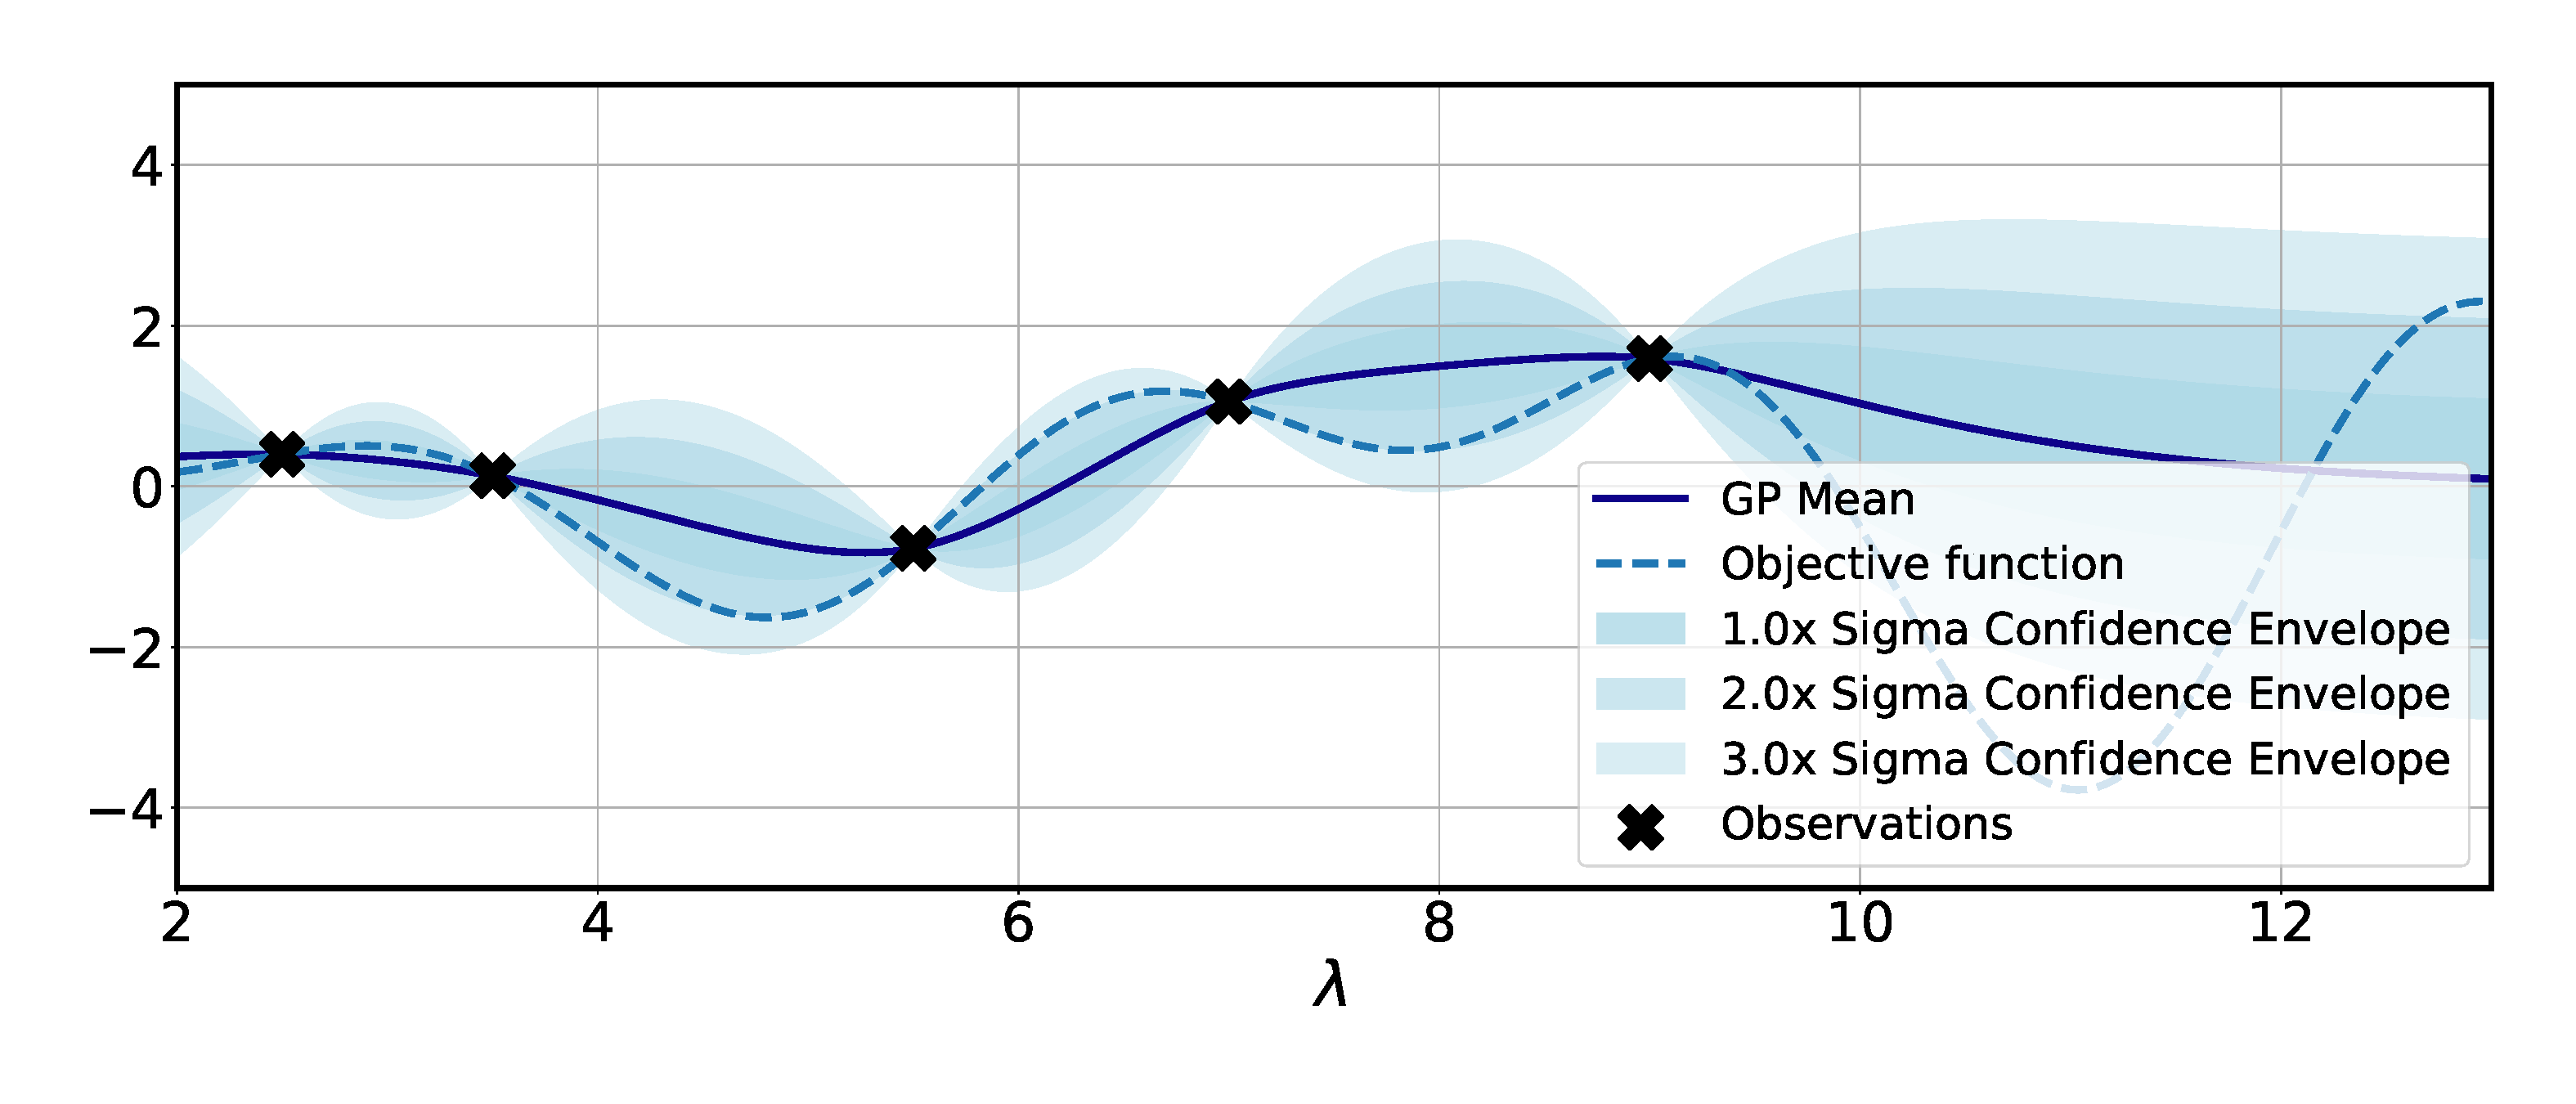
\includegraphics[width=\linewidth, height=0.7\textheight, keepaspectratio=true]{images/acq_func_images/lcb/lcb_1.pdf}};
    \node<.> [below=0.01\belowcaptionskip of img1, align=center]{Given the surrogate fit at iteration $\bocount$};
    %fit on dataset $\iter[\bocount-1]{\dataset}$};
    \node<+> (img2) {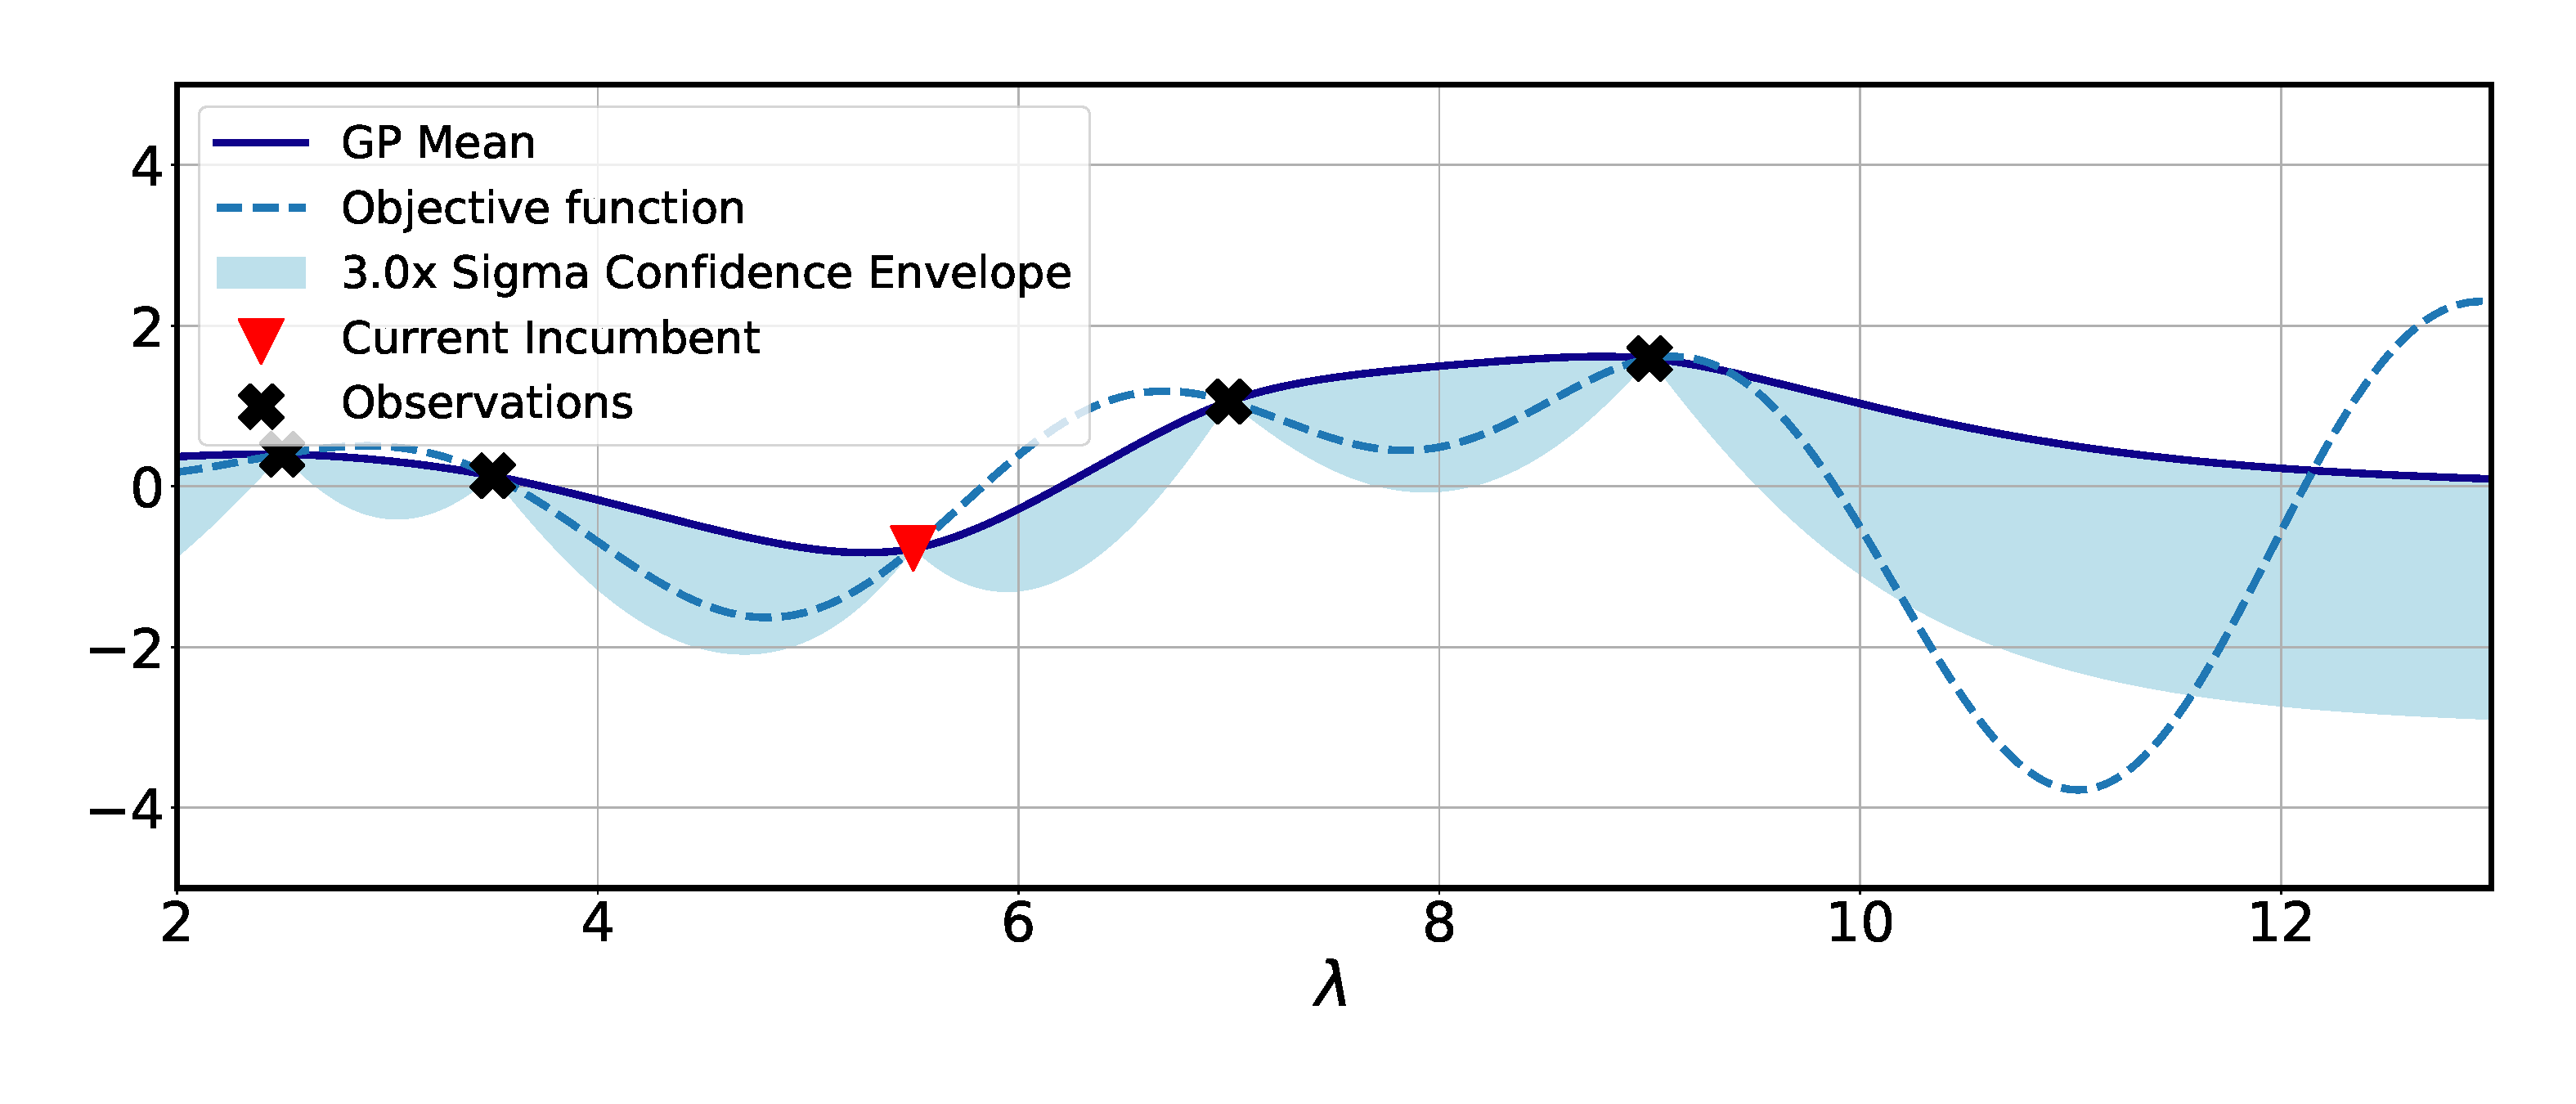
\includegraphics[width=\linewidth, height=0.7\textheight, keepaspectratio=true]{images/acq_func_images/lcb/lcb_2.pdf}};
    \node<.> [below=0.01\belowcaptionskip of img2, align=center]{Lower Confidence Bound, $\mean(\conf)-\alpha\stddev(\conf)$ (here, for $\alpha=3$)};
  \end{tikzpicture}
% \end{figure}

\end{frame}
%-----------------------------------------------------------------------
\begin{frame}[c]{Lower/Upper Confidence Bounds (LCB/UCB): Formal Definition}
\begin{itemize}
    \item We define the \alert{Lower Confidence Bound} as
    \[\alert{\iter{\acq}_{LCB}(\conf) = \iter{\mean}(\conf) - \alpha\iter{\stddev}(\conf)},\quad\alpha\geq0\]

\bigskip
    \item One can schedule $\alpha$ (e.g., increase it over time \lit{\href{https://arxiv.org/pdf/0912.3995.pdf}{Srinivas et al. 2009}})

\[
    \boxed{\text{Choose}\;\;\bonextsample \in \argmax_{\conf\in\pcs}\left(\alert{-} \iter{\acq}_{LCB}(\conf)\right)}
\]

\end{itemize}
    \bigskip
    \pause
    
    \begin{itemize}
    
    
        \item Note: when one aims to \alert{maximize} the objective function, one would use \alert{UCB} instead
        \begin{itemize}
            \item $\iter{\acq}_{UCB}(\conf)) = \iter{\mean}(\conf) + \alpha\iter{\stddev}(\conf)$ 
            \item For UCB, one would choose $\bonextsample \in \argmax_{\conf\in\pcs}( \iter{\acq}_{UCB}(\conf))$ 
        \end{itemize}
    \end{itemize}
   
%    \item It has been shown that using the acquisition function
%    \[\iter{\acq}_{GP-LCB}(\conf) = \iter{\mean}(\conf) - \sqrt{\nu\tau_t}\iter{\stddev}(\conf), \quad\nu>0,\] asymptotically results in zero cumulative regret with the appropriate choice of parameters $\tau$ and $\nu$ \lit{\href{https://arxiv.org/pdf/0912.3995.pdf}{Srinivas et al. 2009}}.}
%    \comment{Trying to further explain the difference between LCB and GP-LCB's parameters would've overwhelmed the intuitiveness of the slide. Instead, a quick verbal note on the difference and pointing out the reference paper by Srinivas et al. for further reading should suffice.}
    %\comment{Source: Tutorial by Brochu et al.: https://arxiv.org/pdf/1012.2599.pdf }
\end{frame}
%-----------------------------------------------------------------------
\begin{frame}[t]{Thompson Sampling (TS): Concept}

% \begin{figure}
  \centering
  \begin{tikzpicture}
    \node<+> (img1) {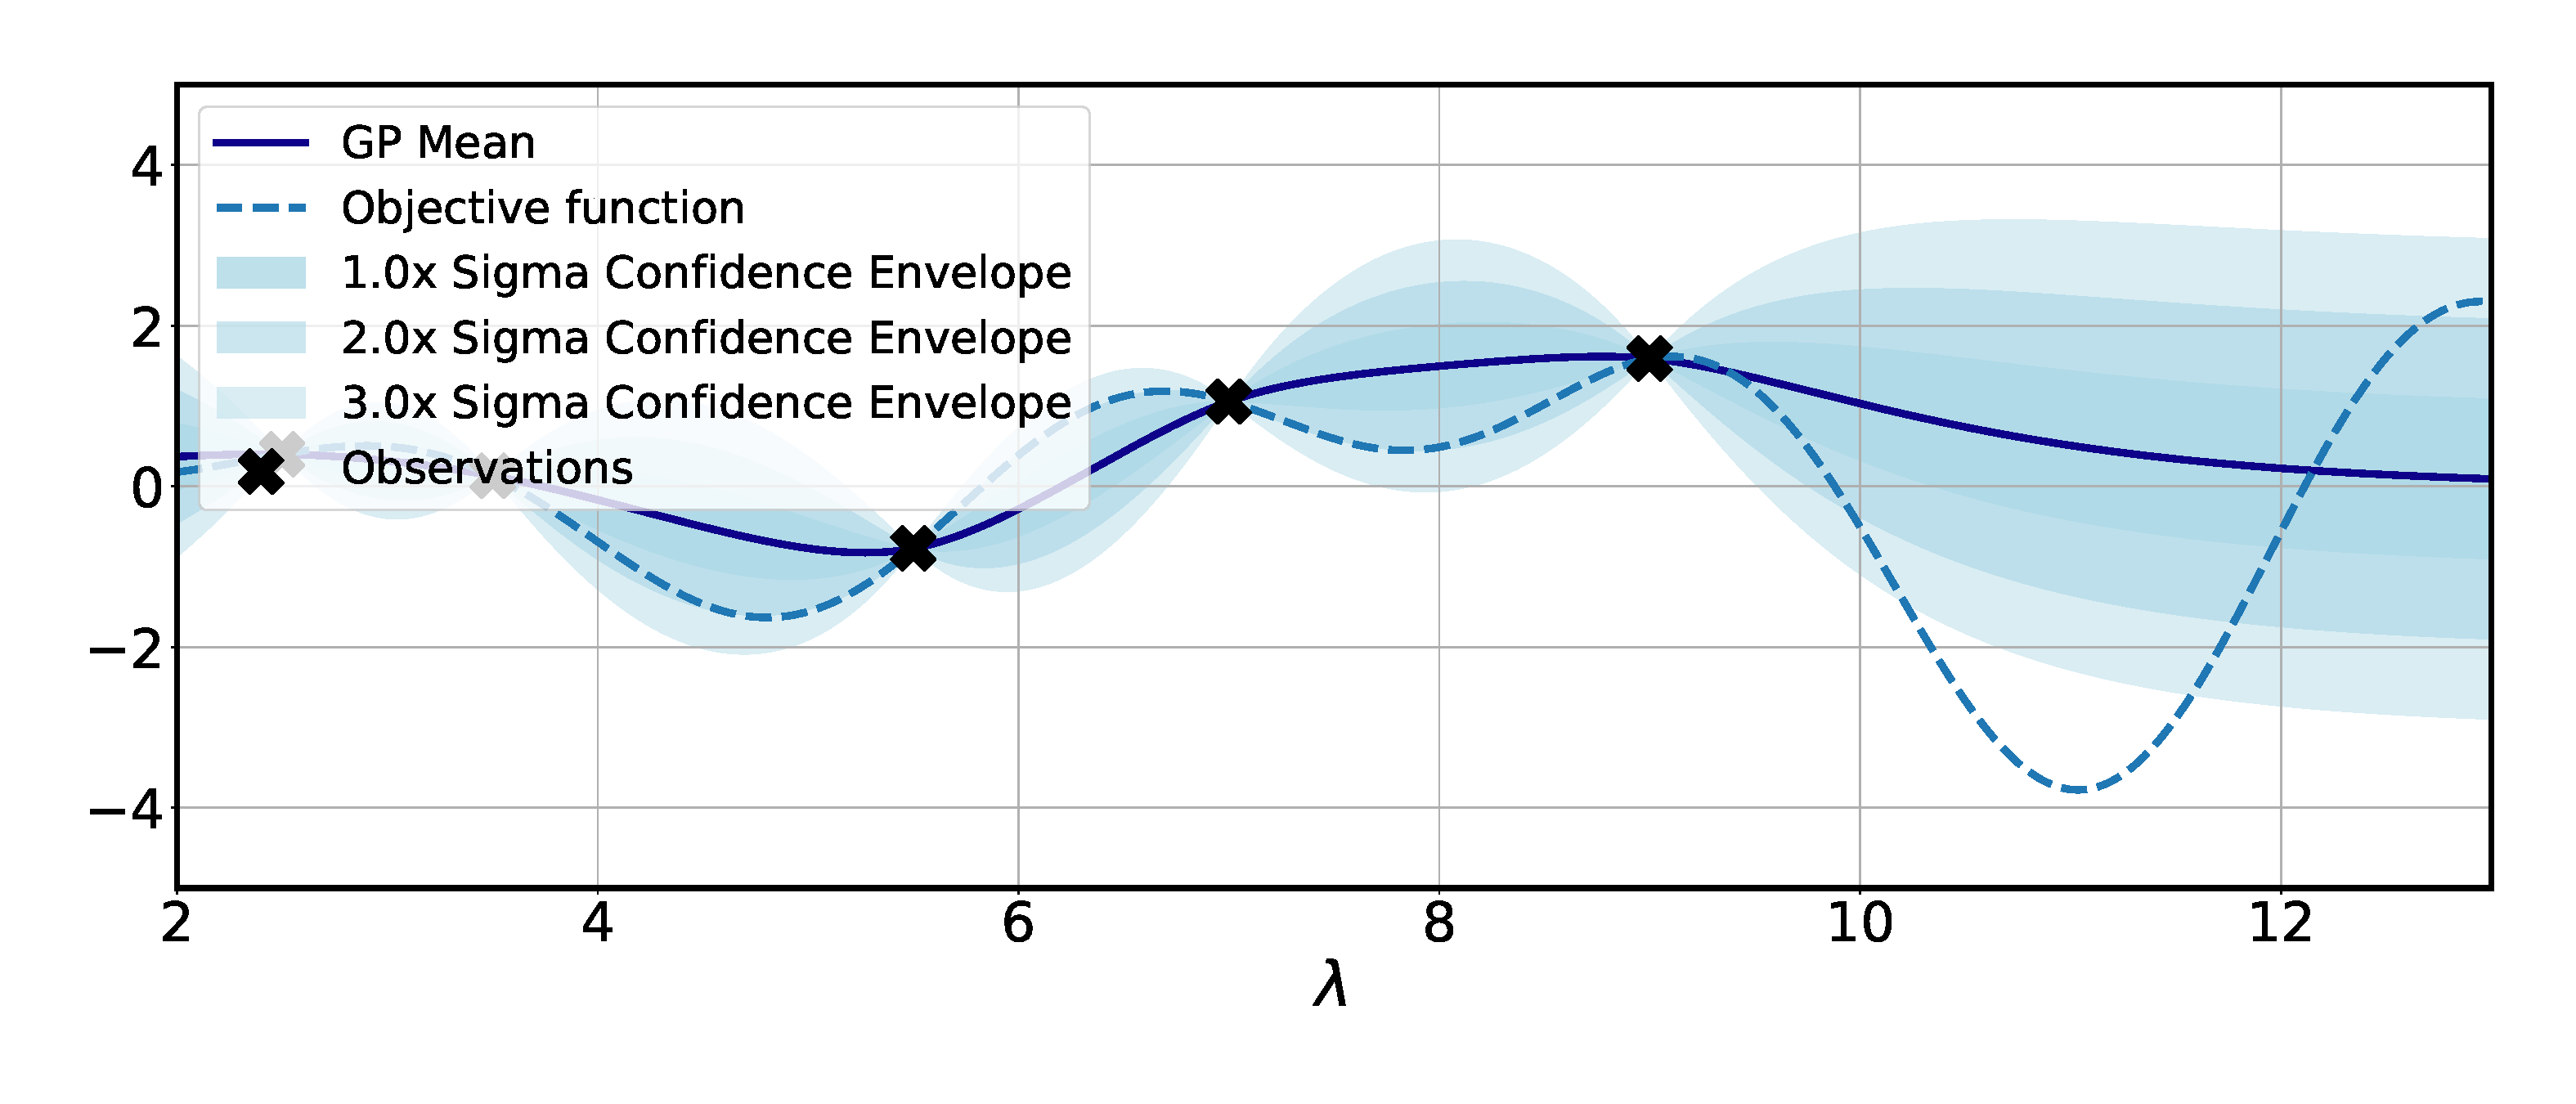
\includegraphics[width=\linewidth, height=0.7\textheight, keepaspectratio=true]{images/acq_func_images/ts/ts_1.pdf}};
    \node<.> [below=0.01\belowcaptionskip of img1, align=center]{Given the surrogate at iteration $\bocount$ fit on dataset $\iter[\bocount-1]{\dataset}$};
    \node<+> (img2) {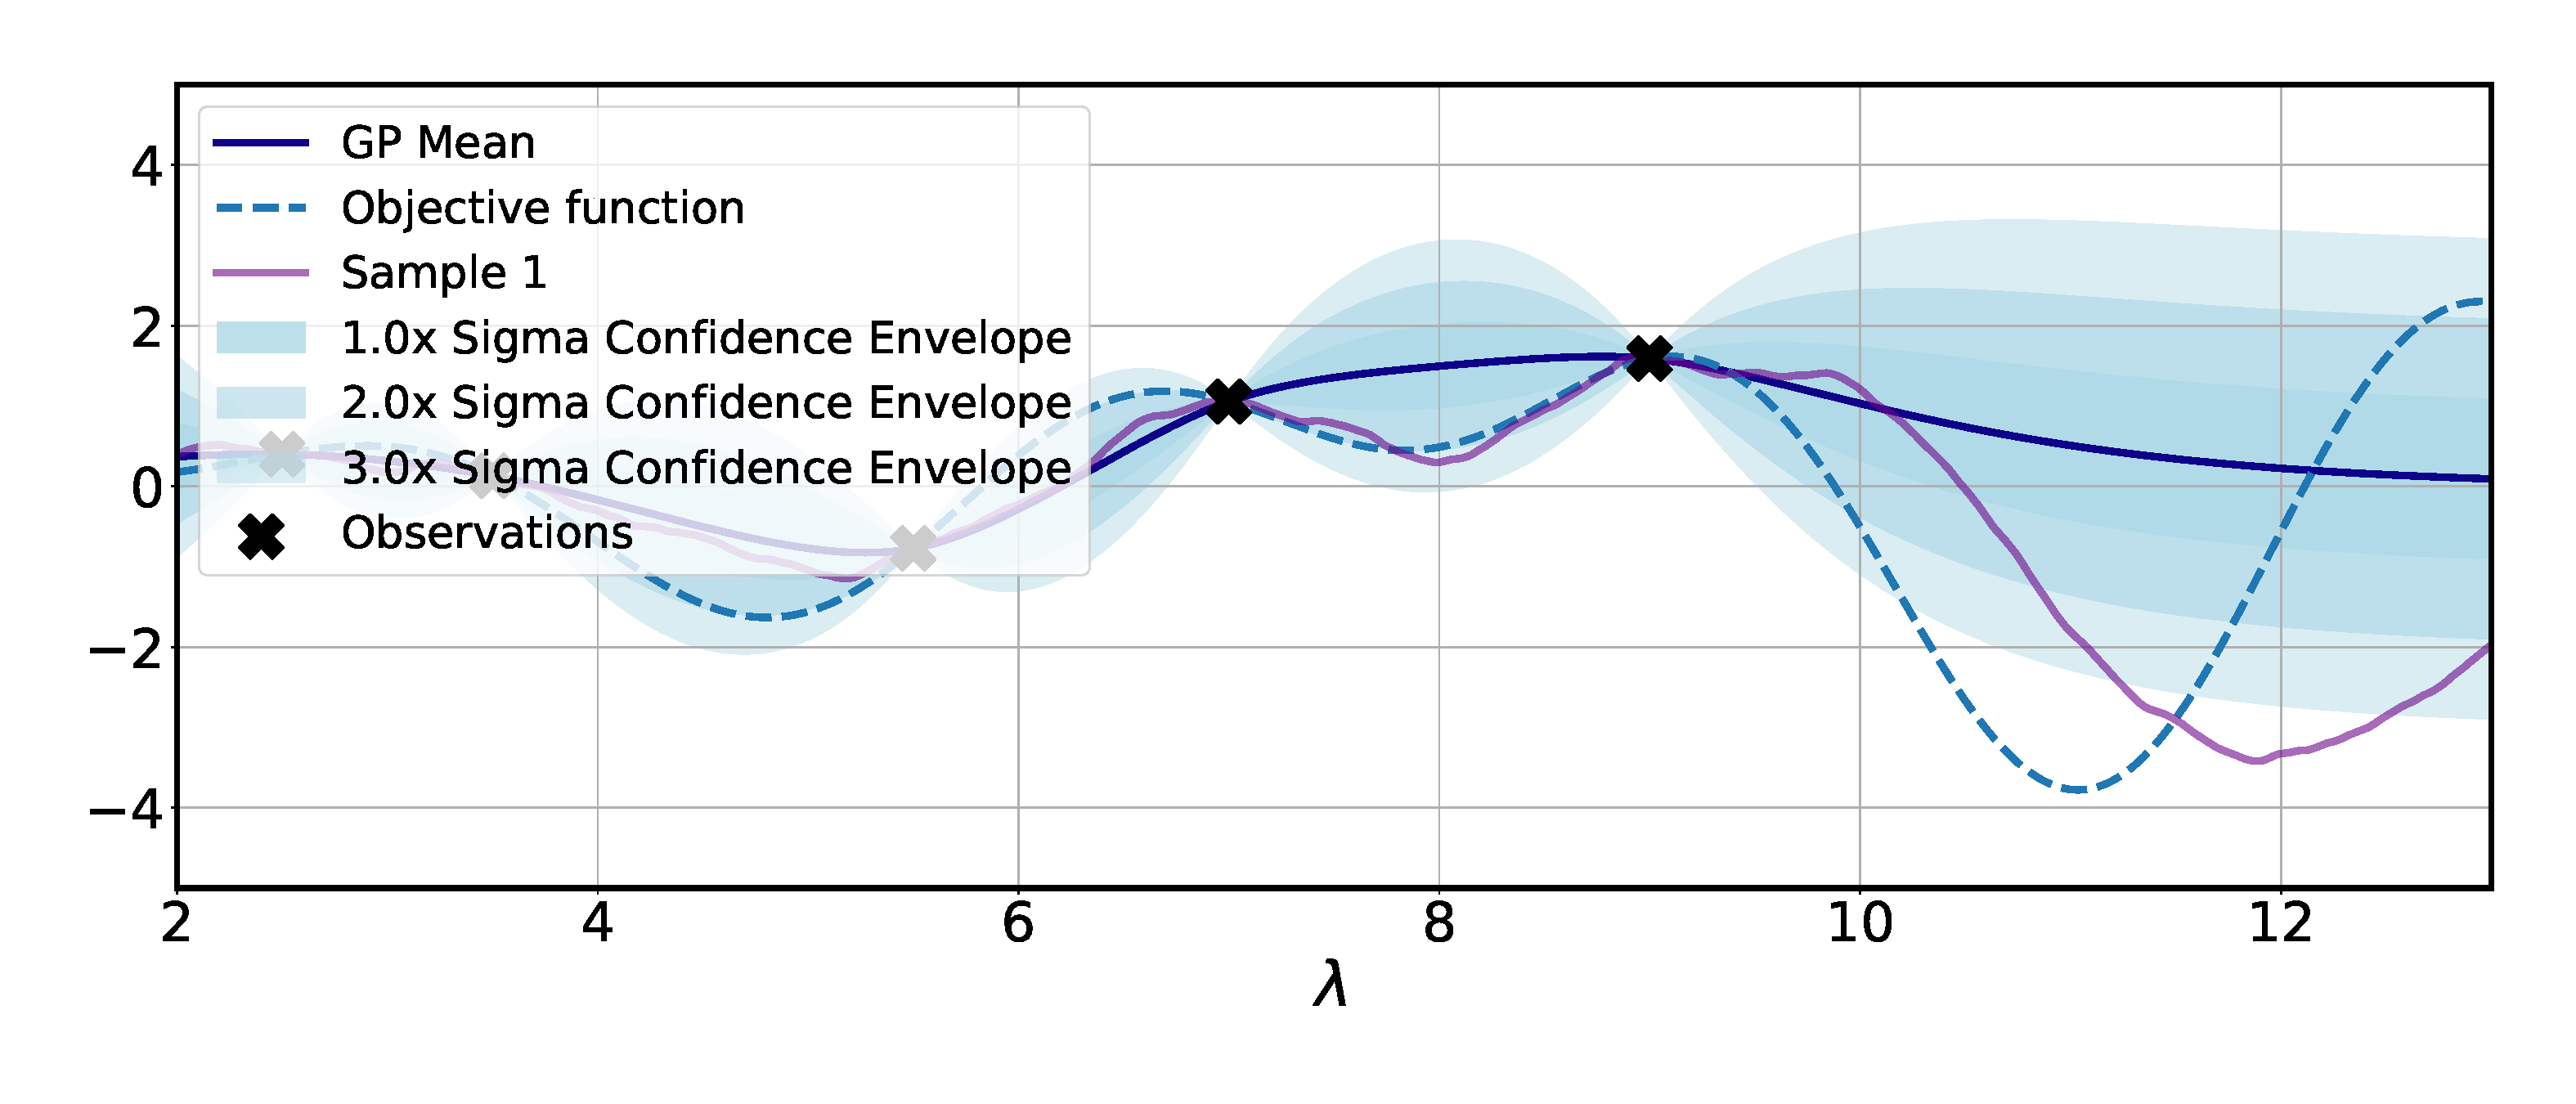
\includegraphics[width=\linewidth, height=0.7\textheight, keepaspectratio=true]{images/acq_func_images/ts/ts_2.pdf}};
    \node<.> [below=0.01\belowcaptionskip of img2, align=center]{Draw a sample $g$ from the predictive surrogate model};
    \node<+> (img3) {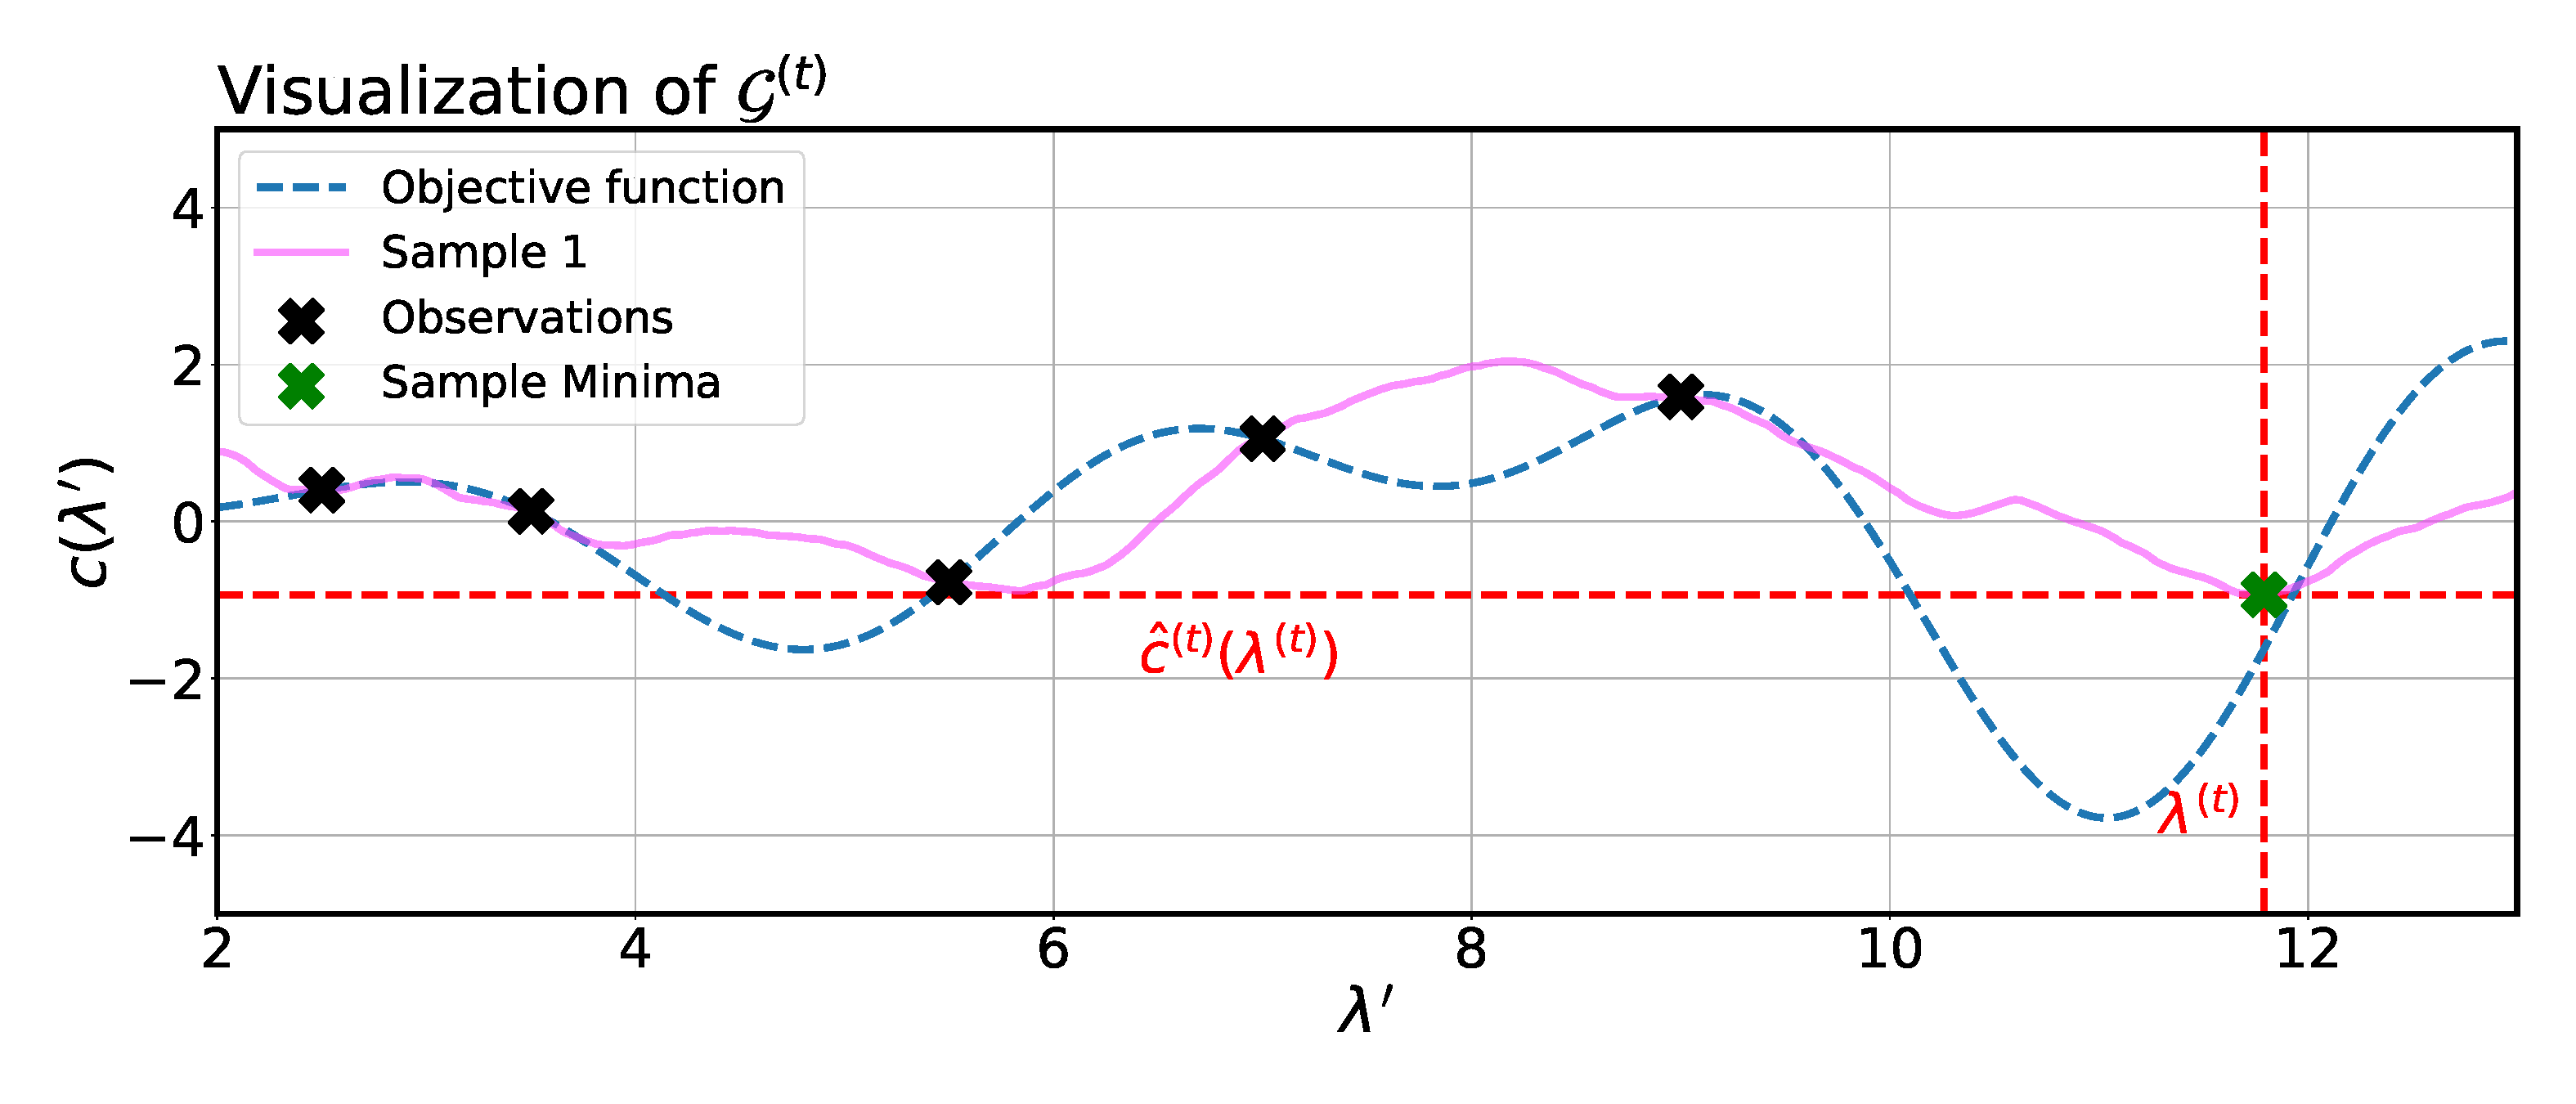
\includegraphics[width=\linewidth, height=0.7\textheight, keepaspectratio=true]{images/acq_func_images/ts/ts_3.pdf}};
    \node<.> [below=0.01\belowcaptionskip of img3, align=center]{Then choose the minimum of this sample to evaluate at next};
  \end{tikzpicture}
% \end{figure}

\end{frame}
%-----------------------------------------------------------------------
% \begin{frame}[c]{Computationally Cheap Acquisition Functions - TS}
% \framesubtitle{Thompson Sampling - Gist}
% 
% \begin{itemize}
%     \item Draw a sample $g$ from the GP $\iter{\gp}$.
%     \item Choose $\bonextsample=\argmin_{\conf\in\pcs}(g(\conf))$
% \end{itemize}
% \end{frame}
%-----------------------------------------------------------------------
\begin{frame}[c]{Thompson Sampling (TS): Pseudocode}

\begin{center}
\begin{minipage}{0.75\textwidth}
\comment{Fix algorithm numbering}
\begin{algorithm}[H]
    %\DontPrintSemicolon
    \LinesNumbered
%    \SetAlgoLined
    \setcounter{AlgoLine}{0}
    \SetKwInOut{Require}{Require}
    \SetKwInOut{Result}{Result}
    
    \Require{Search space $\pcs$, 
    		cost function $\cost$, 
    		surrogate model $\surro$,
    		maximal number of function evaluations $\bobudget$}
\Result{Best observed configuration $\finconf$ according to $\iter[\bobudget]{\dataset}$ or $\gp$}    
	Initialize data $\iter[0]{\dataset}$ with initial observations\;% \leftarrow \varnothing$\; 
    
    \For{$\bocount=1$ \KwTo $\bobudget$}{
    
		Fit predictive model $\iter[\bocount]{\surro}$ on $\iter[\bocount-1]{\dataset}$\;
    
        \textcolor{blue}{Sample a function from the surrogate: $g\sim\iter{\surro}$}\;
    
        \textcolor{blue}{Select next query point: $\bonextsample \in \argmin_{\conf\in\pcs}g(\conf)$}\;
    
        Query $\bonextobs$\;

    	Update data: $\iter[\bocount]{\dataset} \leftarrow \iter[\bocount-1]{\dataset} \cup \{\langle \bonextsample, \bonextobs \rangle \}$\;
        }
    \caption*{Bayesian Optimization using Thompson Sampling}
\end{algorithm}
\end{minipage}
\end{center}
%\comment{Source: Paper, Kandasamy et al, http://proceedings.mlr.press/v84/kandasamy18a/kandasamy18a.pdf}
\end{frame}
%-----------------------------------------------------------------------
\begin{frame}[c]{Questions to Answer for Yourself / Discuss with Friends}

\begin{itemize}
%PI
    \item \alert{Discussion.} How would you set the exploration parameter $\xi$ for PI if you want to avoid too incremental improvements?
\medskip
%EI
    \item \alert{Derivation.} Derive the closed form solution of expected improvement.
\medskip
    \item \alert{Discussion.} In which situations would EI perform substantially differently than PI?
%LCB
%TS
\end{itemize}

\end{frame}
\end{document}